% ****************************************************************************************** % Dissertation template and document class for Princeton University
% Author  : Jeffrey Scott Dwoskin <jdwoskin@princeton.edu>
% Adapted from: http://www.math.princeton.edu/graduate/tex/puthesis.html
% ****************************************************************************************** %


%%% For print copies
%% set 'singlespace' option to set entire thesis to single space, and define "\printmode" to remove all hyperlinks for printed copies of the thesis. Delete all output files before changing this mode -- it will turn hyperref package on and off
\documentclass[10pt,lot, lof, singlespace]{puthesis}
%\newcommand{\printmode}{}

%%% For the electronic copy, use doublespacing, define "\proquestmode" to use outlined links, instead of colored links. 
%\documentclass[12pt,lot, lof]{puthesis}
%\newcommand{\proquestmode}{}
% I prefer proquestmode to be off for electronic copies for normal use, since the colored links are less distracting. However when printed in black and white, the colored links are difficult to read. 

%%% For early drafts without some of the frontmatter
% Also see the "ifodd" command below to disable more frontmatter
%\documentclass[12pt]{puthesis}

%%%%%%%%%%%%%%%%%%%%%%%%%%%%%%%%%%%%%%%%%%%%%%%%%%%%%%%%%%%%%\
%%%% Author & title page info

\title{An integrative `omics approach to quantitative analysis of physiological metabolic flux control}

\submitted{November 2015}  % degree conferral date (January, April, June, September, or November)
\copyrightyear{2015}  % year in which the copyright is secured by publication of the dissertation.
\author{Sean Richard Hackett}
\adviser{Professor Josh Rabinowitz}  %replace with the full name of your adviser
\departmentprefix{Program in}  % defaults to "Department of", but programs need to change this.
\department{Quantitative and Computational Biology}

%%%%%%%%%%%%%%%%%%%%%%%%%%%%%%%%%%%%%%%%%%%%%%%%%%%%%%%%%%%%%\
%%%% Tweak float placements
% From: http://mintaka.sdsu.edu/GF/bibliog/latex/floats.html "Controlling LaTeX Floats"
% and based on: http://www.tex.ac.uk/cgi-bin/texfaq2html?label=floats
% LaTeX defaults listed at: http://people.cs.uu.nl/piet/floats/node1.html

% Alter some LaTeX defaults for better treatment of figures:
    % See p.105 of "TeX Unbound" for suggested values.
    % See pp. 199-200 of Lamport's "LaTeX" book for details.
    %   General parameters, for ALL pages:
    \renewcommand{\topfraction}{0.85}	% max fraction of floats at top
    \renewcommand{\bottomfraction}{0.6}	% max fraction of floats at bottom
    %   Parameters for TEXT pages (not float pages):
    \setcounter{topnumber}{2}
    \setcounter{bottomnumber}{2}
    \setcounter{totalnumber}{4}     % 2 may work better
    \setcounter{dbltopnumber}{2}    % for 2-column pages
    \renewcommand{\dbltopfraction}{0.66}	% fit big float above 2-col. text
    \renewcommand{\textfraction}{0.15}	% allow minimal text w. figs
    %   Parameters for FLOAT pages (not text pages):
    \renewcommand{\floatpagefraction}{0.66}	% require fuller float pages
	% N.B.: floatpagefraction MUST be less than topfraction !!
    \renewcommand{\dblfloatpagefraction}{0.66}	% require fuller float pages

% The documentclass already sets parameters to make a high penalty for widows and orphans. 

%%%%%%%%%%%%%%%%%%%%%%%%%%%%%%%%%%%%%%%%%%%%%%%%%%%%%%%%%%%%%\
%%%% Use packages

%\usepackage{amsfonts}

%%% For figures
\usepackage{graphicx}
%\usepackage{subfig,rotate}

%%% for comments
\usepackage{verbatim}

%%% For tables
\usepackage{multirow}
% Longtable lets you have tables that span multiple pages.
\usepackage{longtable}

% Booktabs produces far nicer tables than the standard LaTeX tables.
%   see: http://en.wikibooks.org/wiki/LaTeX/Tables
\usepackage{booktabs}

%set parameters for longtable:
% default caption width is 4in for longtable, but wider for normal tables
\setlength{\LTcapwidth}{\textwidth}

% Sean packages
\usepackage{outlines} % outlines for organization
\usepackage{color} % for coloring of text
\usepackage{amsmath}
\usepackage{multirow}
\usepackage{outlines}
\usepackage{xfrac}
\usepackage{relsize} % for scaling parts of equations. e.g. \mathlarger
\usepackage{hyperref}
\usepackage{rotating}
\usepackage{array} 
\usepackage[none]{hyphenat}
\usepackage{xr} % so that names figures can be appropriately updated
\usepackage{booktabs}
\usepackage[ruled,vlined]{algorithm2e} % for pseudo-code
\usepackage{xcite} % to use bibliography from main MS
\usepackage{mathtools} %left adjust matrices 
\usepackage{etoolbox}
\usepackage{amsfonts}
\usepackage{subfig}
\usepackage{floatrow}

\usepackage[square, comma, sort&compress]{natbib}		%bibliography

\setlength{\parskip}{2mm}

% Sean custom commands

\newcommand{\fixedspaceword}[2][1]{%
  \begingroup
  \spaceskip=#1\fontdimen2\font
  \xspaceskip=0pt\relax % just to be sure
  #2%
  \endgroup
}

%%%%%%%%%%%%%%%%%%%%%%%%%%%%%%%%%%%%%%%%%%%%%%%%%%%%%%%%%%
%%% Printed vs. online formatting
\ifdefined\printmode

% Printed copy
% url package understands urls (with proper line-breaks) without hyperlinking them
\usepackage{url}


\else

\ifdefined\proquestmode
%ProQuest copy -- http://www.princeton.edu/~mudd/thesis/Submissionguide.pdf

% ProQuest requires a double spaced version (set previously). They will take an electronic copy, so we want links in the pdf, but also copies may be printed or made into microfilm in black and white, so we want outlined links instead of colored links.
\usepackage{hyperref}
\hypersetup{bookmarksnumbered}

% copy the already-set title and author to use in the pdf properties
\makeatletter
\hypersetup{pdftitle=\@title,pdfauthor=\@author}
\makeatother

\else
% Online copy

% adds internal linked references, pdf bookmarks, etc

% turn all references and citations into hyperlinks:
%  -- not for printed copies
% -- automatically includes url package
% options:
%   colorlinks makes links by coloring the text instead of putting a rectangle around the text.
\usepackage{hyperref}
\hypersetup{colorlinks,bookmarksnumbered}

% copy the already-set title and author to use in the pdf properties
\makeatletter
\hypersetup{pdftitle=\@title,pdfauthor=\@author}
\makeatother

% make the page number rather than the text be the link for ToC entries
%\hypersetup{linktocpage}
\fi % proquest or online formatting
\fi % printed or online formatting


%%%%%%%%%%%%%%%%%%%%%%%%%%%%%%%%%%%%%%%%%%%%%%%%%%%%%%%%%%%%%\
%%%% Define commands

% Define any custom commands that you want to use.
% For example, highlight notes for future edits to the thesis
%\newcommand{\todo}[1]{\textbf{\emph{TODO:}#1}}


% create an environment that will indent text
% see: http://latex.computersci.org/Reference/ListEnvironments
% 	\raggedright makes them left aligned instead of justified
\newenvironment{indenttext}{
    \begin{list}{}{ \itemsep 0in \itemindent 0in
    \labelsep 0in \labelwidth 0in
    \listparindent 0in
    \topsep 0in \partopsep 0in \parskip 0in \parsep 0in
    \leftmargin 1em \rightmargin 0in
    \raggedright
    }
    \item
  }
  {\end{list}}

% another environment that's an indented list, with no spaces between items -- if we want multiple items/lines. Useful in tables. Use \item inside the environment.
% 	\raggedright makes them left aligned instead of justified
\newenvironment{indentlist}{
    \begin{list}{}{ \itemsep 0in \itemindent 0in
    \labelsep 0in \labelwidth 0in
    \listparindent 0in
    \topsep 0in \partopsep 0in \parskip 0in \parsep 0in
    \leftmargin 1em \rightmargin 0in
    \raggedright
    }

  }
  {\end{list}}



%%%%%%%%%%%%%%%%%%%%%%%%%%%%%%%%%%%%%%%%%%%%%%%%%%%%%%%%%%%%%\
%%%% Front-matter

% For early drafts, you may want to disable some of the frontmatter. Simply change this to "\ifodd 1" to do so.
%\ifodd 0
\ifodd 1
% front-matter disabled while writing chapters
\renewcommand{\maketitlepage}{}
\renewcommand*{\makecopyrightpage}{}
\renewcommand*{\makeabstract}{}

% you can just skip the \acknowledgements and \dedication commands to leave out these sections.

\else


\abstract{
% Abstract can be any length, but should be max 350 words for a Dissertation for ProQuest's print indicies (150 words for a Master's Thesis) or it will be truncated for those uses.
Advances in genomics continue to make detection of large numbers of related biomolecules (e.g. mRNAs, proteins or metabolites) more routine. While these �omic techniques summarize how the state of one type of biomolecule changes across conditions, they provide a one-dimensional view of cellular processes that emerge at the interface between classes of species. To bridge multiple �omic dimensions, approaches are needed that rationally integrate diverse types of data. In assessing this question, we are interested in testing the validity of models that posit some interaction between diverse chemical species. This process entails not only a rigorous analysis of individual �omic datasets, but also a procedure for posing alternative models and statistically evaluating their relative support. Here, we present a quantitative, scalable strategy for revealing steady-state metabolic regulation by integrating metabolomic, proteomic, and flux measurements. This involves analyzing, on a reaction-by-reaction basis, whether fluxes across conditions are accounted for by a Michaelis-Menten relationship between enzymes, substrates, and potential regulator concentrations. We collected the required data for yeast growing at 25 different nutrient-limited steady states and applied this strategy to reveal the primary physiological flux control mechanisms for over 40 metabolic reactions, encompassing 34 instances of physiologically-relevant allosteric regulation. The identified regulation included classical feedbacks and unexpected cross-pathway connections. Quantitatively, half of flux control resided in substrates and one quarter in enzyme concentrations. For reversible reactions, the remainder resided largely in product levels, and for irreversible reactions, in allosteric effectors. Thus, metabolic activity is substantially self-regulated by metabolites themselves. Across the diverse growth conditions studied, strong changes in mRNA expression generally resulted in corresponding changes in protein abundance. This association between mRNA and protein expression changes, however, was far weaker than expected; the levels of many proteins departed markedly from their cognate transcript. These deviations were highly non-random, suggesting that post-transcriptional regulation has an important role in modulating the cellular response to nutrient availability. This work collectively provides focused examples of how the structures of complex systems can be interrogated to identify meaningful regulatory relationships.  And, it is at the interface between �omic datasets that these valuable relations emerge.
}

\acknowledgements{
%I would like to thank...
I am very grateful to the members of the Rabinowitz, Storey and Botstein groups as well as other members of the Lewis-Sigler Institute for providing contrasting perspectives that naturally support interdisciplinary thinking. Working in this environment has refined my scientific interests and set me on a lifelong path of probing inspiring scientific questions.

I would like to begin by thanking my advisor, Josh Rabinowitz, whose support and direction have shaped my project immensely. Josh paralleled my interest in metabolic systems biology, providing motivation and direction towards a meaningful, shared goal. A masterful communicator, Josh has refined the scope of my scientific expression: verbally, visually and linguistically.

John Storey can also not go without acklowledgement; John introduced me to statistical methods and approaches of visualization which revolutionized my approach to research. Being a fly on the wall at his group meetings helped me think about questions in a statistical manner. 

I would like to thank all past and present members of the Rabinowitz research group for their advice and support over the past five years. I would like to further highlight the formative contributions of several individuals. Vito Zanotelli provided enormous support by establishing a formalism for analyzing reaction kinetics. He helped assemble summaries of literature regulation and implemented approaches to deal with flux uncertainty. Wenxin Xu has helped with verifying regulatory predictions and testing the validity of flux estimation methods. Chel Nofal has been an invaluable sounding board for evaluating the merit and delivery of results. Ian Lewis assisted with the experimental measurement of media samples using NMR. I am also extremely grateful to Greg Ducker, Lukas Tanner, Xiaoyang Su, Yifan Xu, Chris Crutchfield and Meytal Higgens for helping with experimental methods.

Other members of the Lewis-Sigler Institute have enormously helped my work and development at Princeton: David Bostein set me on the path to thinking about biology in a quantitative manner and helped me to understand the awesome power of yeast genetics. Pat Gibney taught me how use yeast genetics; he made several of the expression strains used to test regulation and provided invaluable experimental advice on all things yeast. Dave Robinson provided programming advice and was always available and ready to think about statistical questions with me. Jonathan Goya helped run many of the chemostat experiments, was an integral part of the proteomics analysis and helped me think about the quantitative relationship between proteins and transcripts. David Perlman provided a plethora of advice on setting up proteomics experiments and spent a huge amount of effort to ensure that the dataset was top notch. Sandy Silverman taught me how to do numerous yeast experiments. I would also like to thank Keyur Desai and Peter Andolfatto for their guidance.

I would like to thank the great administrators whose helped me easily navigate bureaucratic challenges, including Marybeth Fidele, Jen Brick and Ping Ge.

I would also like to sincerely thank my past scientific mentors, who set me on the path to a PhD by making me see the intrigue of science. As an undergraduate, Teresa Gunn helped turn my interest in genetics into an interest in scientific discovery. Andy Clark taught me to think about grand questions and how to interrogate them using appropriate large datasets. Tony Greenberg fostered my interest in statistics, programming (and Brazillian Jiu-Jitsu).

I would also like to thank my family. As the son of two veterinarians,  I was instilled with a keen interest in biology that provided me direction through college and beyond. Finally, I want thank my fianc\'{e}, Maya, whose presence gave me perspective throughout my graduate education and whose proofreading efforts will hopefully make the reading of this dissertation more enjoyable.

This research is based upon work supported by the U.S. Department of Energy, Office of Science, Office of Biological and Environmental Research (BER), under Award Number DE-SC0012461. This research was supported in part by an award from the Department of Energy (DOE) Office of Science Graduate Fellowship Program (DOE SCGF). The DOE SCGF Program was made possible in part by the American Recovery and Reinvestment Act of 2009.  The DOE SCGF program is administered by the Oak Ridge Institute for Science and Education for the DOE. ORISE is managed by Oak Ridge Associated Universities (ORAU) under DOE contract number DE-AC05-06OR23100.  All opinions expressed in this work are the author's and do not necessarily reflect the policies and views of DOE, ORAU, or ORISE.
}

%\dedication{}

\fi  % disable frontmatter


%%%%%%%%%%%%%%%%%%%%%%%%%%%%%%%%%%%%%%%%%%%%%%%%%%%%%%%%%%%%%\
%%%% Hide some chapters

%%% If you want to produce a pdf that includes only certain chapters, specify them with includeonly, in addition to including all chapters below.
%\includeonly{ch-quant_anal/quant_analysis, ch-intro/chapter-intro}
\includeonly{ch-conclusion/chapter-conclusion, ch-intro/chapter-intro}
%%% You can also specify multiple chapters.
%\includeonly{ch-intro/chapter-intro,ch-usage/chapter-usage}
%\includeonly{chap1,chap2,chap3}


%%%%%%%%%%%%%%%%%%%%%%%%%%%%%%%%%%%%%%%%%%%%%%%%%%%%%%%%%%%%%
%%%% Notes:

% Footnotes should be placed after punctuation.\footnote{place here.}
% Generally, place citations before the period~\cite{anotherauthor}.
% The proper usage for i.e., and e.g., include commas ``(e.g., option A, option B)''

%%%%%%%%%%%%%%%%%%%%%%%%%%%%%%%%%%%%%%%%%%%%%%%%%%%%%%%%%%%%%
%%%% Import chapters

\begin{document}

\makefrontmatter


% If you've disabled frontmatter, you can insert the toc manually
%\tableofcontents\clearpage

% \include lets us split up the document (and each include starts a new page):

\chapter{Introduction\label{ch:intro}}

As an undergraduate genetics major I became fascinated with complex traits and diseases such as height, corn yield and heart attack risk. While these traits are of huge societal importance, each is collectively determined by numerous genetic variants and environmental factors and consequently relating quantitative traits to their genetic determinants has been notoriously difficult \cite{Manolio:2009jp}. As I began at Princeton, I wanted to better understand the source of missing heritability and how the explanatory insufficiency of the GWAS paradigm may be better addressed. My insight into this problem was that the gulf separating genetic variation and whole-body complex traits is the massive complexity of organismal and cellular physiology.

At the scale of cellular and organism-level systems, thousands of genes and environmental effects collide leading to non-additive, non-linear interactions, such as those resulting in canalization \cite{Waddington:1942wy}. Because the outputs of these systems cannot be explained using additive genetics, the combination of many such sub-systems into organism-level phenotypes will only further distort the relationship between individual genetic variants and overall phenotypic variability. Outside of tightly controlled studies of microbial growth \cite{Bloom:2013bq} it is likely that additive genetics can only explain a minority of many phenotype's variation regardless of statistical power \cite{Weedon:2008gc,WellcomeTrustCaseControlConsortium:2007do}. Furthermore, genome-scale methods which attempt to account for such non-additive and non-linear interactions will be unable to rigorously detect such interactions because of the massive space of such interactions \cite{Friedman:1997kn}. An alternative to this unsupervised approach can be found in systems biology, where researchers continually build bottom-up models of systems operations based on a relatively small number of inputs.

\subsection{Harnessing the power of systems biology}

A single systems biology model may focus on a minute aspect of an organism, such as how the expression of a single gene, your favorite gene (YFG), is determined based on the activity of its primary transcriptional repressor and cis-regulatory variation in YFG \cite{Nuzhdin:2012ii}. Such a simple model of YFG expression can be used to characterize YFG protein abundance \cite{Jovanovic:2015hp}, which can in turn be built into a model of signaling or metabolic pathway activity \cite{Neves:2002bk, Chassagnole:2002ty}.  The importance of each model is that it integrates information within the appropriate context of the systems operation, allowing changes in system output (and uncertainty) to be expressed as a non-linear function of variation in inputs.

In a perfect world where systems are well understood, genetic and environmental variants could be propagated through individual subsystems, appropriately aggregating information and ultimately allowing for accurate prediction of quantitative traits and disease risk.  Importantly, at such a juncture, prediction would require far less data than would be necessary to initially parameterize the system. This utopian vision of systems biology is quite removed from reality, as the creation of systems-level models is hindered by both extensive experimental requirements and general challenges in model identification.

The need for extensive experimentation and challenges in model discovery lay at odds in experimental design, as given fixed resources, there are tradeoffs between producing an experiment which measures all of the desired variables and characterizing a sufficient number of conditions (and replicates) to distill anything meaningful from the quantitative information. This problem is further exacerbated as funding is further distributed among groups characterizing different systems, in different organisms, with limited direct cross-domain translatability. 

To simplify the complex model inference problems of systems biology, I adopted an experimentally-guided reductionist approach. Essentially, by acquiring more data, we can actually get away with analyzing fewer distinct conditions, by breaking complicated systems-level model inference questions into simpler sub-problems. To illustrate this reoccurring theme, consider the inference of metabolic regulation, the major topic of \hyperref[ch:simmer]{Chapter \ref{ch:simmer}}. If we are interested in identifying which of 50 metabolites ($m$) regulates each of 50 reactions of interest ($n$), then 2500, $\mathcal{O}(nm)$, possible metabolite-reaction pairs exist. This scale of inference is highly tractable, however, using existing approaches metabolic regulation is primarily tested at a systems-level (i.e. as a combined model-fit over all 50 reactions) \cite{Link:2013dj, Zampar:2013fr}.  In this case, the number of sets of possible regulatory relationships that could exist is 8.88 $\times 10^{84}$, $\mathcal{O}(n^{m})$, similar to the number of atoms in the observable universe. To make this problem scalable, I was able to achieve $\mathcal{O}(nm)$ complexity by breaking the dependence between reactions through measuring metabolic fluxes, rather than treating them as latent variables.

\subsection{Towards understanding how metabolism is controlled}

To allow for the application of piecewise inference, I focused on studying the baker's yeast, \textit{S. cerevisiae}, as a simple eukaryote that can be easily cultured and is amenable to genetic manipulation. Previous research in the Rabinowitz and Botstein groups has shown that when yeast are cultured in chemostats with greatly varying nutrient availability, both the transcriptome and metabolome are radically affected, but in a distinct manner \cite{Brauer:2008jn, Boer:2010fb}. Across these cultures, differences in growth rate and which nutrient is limiting growth (such as a carbon or nitrogen source), yields a panel of diverse physiological and metabolic states. As growth rates change, the transcriptome is strongly affected, with many transcripts increasing or decreasing in a log-linear fashion with growth rate, irrespective of which nutrient limits growth \cite{Brauer:2008jn}. In contrast, the metabolome is profoundly affected by which nutrient limits growth, with distinct metabolites appearing to be growth-limiting or overflowing depending on which primary nutrient limits growth \cite{Boer:2010fb}. While these studies convey the importance of both transcription and metabolism in nutrient-dependent growth control, each dataset is only able to provide a 1-dimensional answer to a question that inherently involves multiple `omic dimensions.

When yeast are growing at different rates and in media of greatly differing composition, they face a massive metabolic challenge. When growing quickly, metabolic rates (fluxes) must increase to produce enough  proteins, RNAs and other biomass components to keep pace with dilution.  Moreover, metabolic pathways must generally maintain an appropriate balance of energy, reducing equivalents and biomass components, across a broad spectrum of possible environments and genetic states. To achieve such fine control, pathway fluxes are collectively determined by enzyme expression, nutrient availability and metabolic regulation.  While analysis at this scale has been used to investigate the coordinated regulation of specific metabolic events involving small sets of genes \cite{Zampar:2013fr, Link:2013dj} as previously discussed this approach is ill suited to identifying novel regulation and reaction kinetics at scale. Instead, pathway-level regulation can be considered as an emergent property of interactions between reactions, where reaction-level kinetics are sufficient to reconstruct higher-order behavior \cite{Fell:1997wg}.

To characterize individual reactions, we can assess whether a model of reaction kinetics, such as Michaelis-Menten kinetics (\hyperref[intoEqtn:mm]{Equation \ref{intoEqtn:mm}}), is able to accurately predict the model output (flux) as a function of model inputs (metabolite and enzyme concentrations) and kinetic parameters \cite{Anonymous:1913wn, Liebermeister:2006fm, Tummler:2014cp}. Here, $\nu$ is the reaction flux, $\left[E\right]$ is the enzyme's concentration, k$_{cat}$ is the per-enzyme maximum rate of conversion of substrates into products ($\sfrac{1}{s}$), $\left[S\right]$ is the substrate's concentration, and k$_{m}$ is effectively the concentration where half of enzymes are bound by substrates.

\begin{equation}
\nu = k_{cat}\left[E\right]\frac{\left[S\right]}{\left[S\right] + k_{m}}\label{intoEqtn:mm}
\end{equation}

Under this simplified kinetic model, variable flux could be accomplished through two simple regulatory paradigms: either the concentration of enzymes changes proportionally to their flux, or the fractional substrate occupancy of each enzyme increases. For this second hypothesis, the upstream accumulation of metabolites could be a driving force that is directly controlled by nutrient availability. A combination of these strategies is also possible, where different enzymes could employ one or both of these methods of flux-control. 

Previous work from our laboratory, using transcript levels as an approximation of protein levels, has revealed that neither of these simple paradigms is generally consistent with inferred reaction fluxes \cite{Bradley:2009fj}. There is no consistent relationship between fluxes and transcript abundance for most enzymes, nor do metabolites reliably accumulate upstream of enzymes as flux increases. This suggests that either transcript abundance is an unsuitable surrogate for enzyme abundance (a hypothesis that can be tested using protemics) or that we need to expand the model beyond simple Michaelis-Menten kinetics to account for other mechanisms of flux regulation, such as post-translational modifications, allostery and localization. Across different nutritional conditions, we must consider not just the differences in flux associated with growth rate, but also potential differences in flux due variable cellular composition and energetics, such as tradeoffs between fermentation and respiration \cite{Lange:2001th, Feist:2010hq, BARFORD:1979ei}.

\subsection{Integrative `omic approaches to identify metabolic and post-transcriptional regulation}

While analysis of transcriptional and metabolomic variation suggested that existing yeast chemostat conditions would be an ideal system to investigate the regulatory underpinnings of nutrient-based growth control, additional data was required if we were to meaningfully address this question. To greatly reduce the gaps in our knowledge, I measured protein abundance across the 25 chemostat conditions using quantitative proteomics and estimated metabolism-wide fluxes using flux balance analysis (\hyperref[introFig:primarytopics]{Figure \ref{introFig:primarytopics}A}) \cite{Orth:2010hb}. As metabolite and enzyme concentrations are the primary determinants of reaction flux, the appropriate quantification of these species using mass spectrometry is a major focus of my research. During \hyperref[ch:quant_anal]{Chapter \ref{ch:quant_anal}} I discuss appropriate methods for analyzing mass spectrometry data and highlight my collaborations where metabolomics or proteomics provided novel insights into physiology and evolution. 

During \hyperref[ch:simmer]{Chapter \ref{ch:simmer}}, I discuss the integration of reaction flux with enzyme and metabolite concentrations to test alternative models of reaction-level kinetics. The first aim of this study is determine whether generalizations of Michaelis-Menten kinetics (\hyperref[intoEqtn:mm]{Equation \ref{intoEqtn:mm}}) \cite{Liebermeister:2006fm} are sufficient to quantitatively related physiological concentrations of substrates and enzymes to variable reaction flux.  To the extent that such an agreement is not possible, I then assessed whether metabolic regulation through allostery is able meaningful improve fit (\hyperref[introFig:primarytopics]{Figure \ref{introFig:primarytopics}B}).  This approach, called SIMMER (\underline{S}ystematic \underline{I}nference of \underline{M}eaningful \underline{M}etabolic \underline{E}nzyme \underline{R}egulation) is novel in that it is able to to scalably identify metabolic regulation. Accordingly, this approach was used to both confirm the physiological important of canonical yeast metabolic regulation and to identify novel regulation which was subsequently experimentally validated. By inferring reaction kinetics based on physiological variation in reaction species, SIMMER also naturally indicates the relative influence of substrates, products, enzymes and regulators in changing reaction flux. This suggests that metabolic activity is largely determined by changes in substrate and product concentrations based on local metabolic context, with direct regulation through regulated changes in protein abundance and allostery primarily acting to fine-tune metabolic behavior.

By deciding to directly measure protein abundance across the chemostat conditions, rather than relying upon transcript abundance as a surrogate for protein abundance I was guarding against possible deviations between protein and transcript abundance. Once protein relative abundance was measured, I was able to compare transcriptional changes to corresponding changes in protein abundance to assess whether the addition of proteomics was necessary (\hyperref[introFig:primarytopics]{Figure \ref{introFig:primarytopics}C}). The results of this analysis are presented in \hyperref[ch:pt_compare]{Chapter \ref{ch:pt_compare}}.  While strong transcriptional changes do indeed propagate into a corresponding change in protein abundance, additional regulation appears to be operating at the post-transcriptional level to further attune transcriptional responses to the metabolic environment. Regulation of protein degradation appears to be particularly important during nitrogen-limitation, where ribosomes are preferentially degraded and metabolic enzymes are selectively retained.

Code supporting each chapter is maintained on \href{https://github.com/shackett}{github}, access to private repositories is available upon request.

\begin{figure}[h!]
\floatbox[{\capbeside\thisfloatsetup{capbesideposition={right,top},capbesidewidth=4cm}}]{figure}[\FBwidth]
{\caption[Summary of primary thesis topics]{\fixedspaceword{\\Summary of primary thesis topics. \textbf{A)} A multi-omic data was generated involving four distinct classes of high-dimensional data. Previously measured transcript and metabolite relative abundances \cite{Brauer:2008jn, Boer:2010fb} were supplemented with measurements of enzyme relative abundances and inference of metabolism-wide fluxes. Each data type was measured across 25 standard chemostat conditions. \textbf{B)} Integration of metabolite, enzymes and flux measurements allows testing of reaction-level models of kinetics. Each possible model of kinetics is described as a non-linear function of substrates, products, enzymes, possible regulators and constants. Alternative kinetic models are compared based on model plausibility, $Pr(Model)$, and how well measured fluxes agree with the Michaelis-Menten kinetics, $Pr(Data | Model)$. \textbf{C)} The relationship between changes in transcript abundance and protein abundance can be modeled using differential equations. Departures between protein and transcript changes may reflect additional post-transcriptional regulated due to variable translational efficiency or protein degradation.
}}\label{introFig:primarytopics}}
{\includegraphics[width=\textwidth-4cm]{ch-intro/Figures/globalQuant.pdf}}
\end{figure}



\chapter{Statistical Analysis of Mass Spectrometry Data\label{ch:quant_anal}}

Mass spectrometry is a powerful way to detect and quantify chemically heterogenous species, particularly metabolites and peptides derived from proteins. Species are distinguished and quantified by exploiting the fact that when placed in a constant electric or magnetic field, ions with the different mass-to-charge ratio (\sfrac{m}{z}) will accelerate at different rates.  Ions that move at different rates can then be quantified by detecting the frequency of their  about an orbitrap or based on differences in their time-of-flight.  Because multiple chemical species can have very similar, or identical, \sfrac{m}{z} and thus cannot be resolved by mass spectrometry, further discrimination of species is possible by using liquid or gas chromatography.  When chromatography is utilized, species are further separated based on retention time (RT), resulting from differential affinity for the chromatography column/solvent, and thus different suites of species will reach the detector in each time slice.  Quantitatively, a single LC-MS run effectively yields a matrix of \sfrac{m}{z} x RT where values are the number of ions detected.  

To effectively use mass spectrometry data, each ion must first be identified. To determine the identity of ions corresponding to mass spectrometry peaks, emerging out of the \sfrac{m}{z} x RT plane, two primary approaches are used.  When studying metabolites, most species of interest, such as amino acids and metabolites in glycolysis, are shared between species and pure standards can be acquired.  By subjecting purified standards to LC- or GC-MS, the characteristic retention time of these species can be found, allowing the identification of ions in subsequent experiments based on shared retention time and exact mass of standards.  When obtaining pure standards of the species of interest is not feasible, such as when many peptides are measured, tandem-mass spectrometry can be used to yield structural information of unknown ions.  Once a subset of the detected ions have been identified as metabolites or peptides, the abundances of these meaningful species can be compared to determine how experimental samples differ.

To illustrate the challenges and opportunities of mass spectrometry, in this chapter I will address the statistical nature of mass spectrometry data, and the application of mass spectrometry to investigate challenging biological questions.  While mass spectrometry data can be approximately modeled with a log-normal distribution, there is an excess of ``outliers'' which if not properly addressed could muddle statistical analysis \textcolor{red}{cite}. During the first section of this chapter, I will discuss the magnitude of deviations from log-normality and discuss the use of variance modeling to describe the excess uncertainty of ``outlier'' observations.  During the second section, I will briefly discuss four studies that I have coauthored that utilized either proteomics or metabolomics to provide insights into native physiology or metabolism. In these four studies, several non-parametric alternatives to variance modeling are used including permutation testing, bootstrapping and even just using median averaging.

\section{Statistical properties of Mass Spectrometry Data}

\subsection{Background}

As biologists continue to search for a deeper understanding of their system, there is an increasing focus on analyzing the proteins and metabolites that are the primary effectors of physiology and metabolism. This increased interest has been enabled by improved analytical techniques for measuring these species, particularly liquid/gas chromatography (GC/LC) coupled mass spectrometry (MS). While the promise of mass spectrometry is great, the community is far from reaching a consensus on how mass spectrometry data should be best analyzed.  Issues of inconsistent treatment include what distribution mass spectrometry data supposedly follows, sources of variation and in proteomics; how peptide-level information should be aggregated to estimate protein abundance. More troubling than these general inconsistencies, is the absence of side-by-side comparisons of alternative methods and a general lack of evaluation of parametric model assumptions. 

Modern approaches to quantitatively model protein, peptide, or metabolite relative abundance generally focus on treating mass spectrometry data as approximately log-normal \cite{Cox:2008ir, Oberg:2012bm,Navarro:2014ke, Breunig:2014bu}, or analyzing protein spectral counts as a quasipoisson trait \cite{Li:2010bj}. Across those approaches which model mass spectrometry data as approximately log-normal, variation at two levels has been previously considered; peptide-level variance and signal-intensity dependent variance \cite{Oberg:2012bm,Navarro:2014ke}. While one or both of these sources of variation are frequently ignored \cite{Oberg:2012bm}, there is an increasing effort to account for the combined influence of multiple variance components \cite{Navarro:2014ke}. While such approaches are likely important, studies to data have failed to clarify whether under the assumed variance model, approximate log-normality is justified. Additionally, it is unclear whether peptide-level variance or signal-intensity dependent variance is the most relevant force of variable uncertainty in mass spectrometry data.

To benchmark alternative statistical approaches for analyzing mass spectrometry data, three moderately sized mass spectrometry experiments (Table \ref{ch-quant_anal:mass_spec_design}) were investigated using a standardized workflow (Figure \ref{ch-quant_anal:MSworkflow_p1}) which allowed for direct model comparison and assumption evaluation.  The three \textit{S. cerevisiae} datasets used for this analysis were: (1) Boer et al. 2010, which examined the role of variable chemostat nutrient environment in driving metabolomic variation; (2) Hackett et al. 2015, further described in thesis chapter \ref{ch:simmer}, which similar to Boer et al. 2010 investigated how protein levels were affected by nutrient environment; (3) Foss et al. 2007, which investigated how levels of proteins are impacted by segregating variation between two parental strains. These datasets differ in terms of whether metabolites or peptides are analyzed and vary greatly in terms of both number of features and samples analyzed, thereby providing a good survey of the variable needs in mass spectrometry data analysis. The aim of each dataset is to estimate the relative abundance of features for each level of the the main effect while also minimizing the added variation introduced into the data from random block-specific effects (Equation \ref{eq:mass_spec_design}). 

\begin{table}[h!]
\begin{center}
\resizebox{\columnwidth}{!}{
\begin{tabular}{| l| l| l| l| c |}
  \hline
  Dataset & Type & Features & Samples & Model\\
  \hline			
  Boer et al. 2010 & Metabolites & 101 & 136 & $X \sim Condition + Method + (1|Block) + \epsilon$ \\
  Hackett (\ref{ch:simmer}) & Peptides & 11168 & 75 & $X \sim Condition + (1|Block) + \epsilon$\\
  Fell et al. 2007 & Peptides & 5279 & 448 & $X \sim Segregant + (1|BioRep) + \epsilon$ \\
  \hline
\end{tabular}
}
\caption[Summary of benchmark datasets]{Summary of benchmark datasets}
\label{ch-quant_anal:mass_spec_design}
\end{center}
\end{table}


\begin{figure}[h!]
\begin{center}
\includegraphics[width = 1\textwidth]{ch-quant_anal/Figures/MSanalysis_part1.pdf}
\caption[Schematic representation of peptide and metabolite level analysis]{Schematic representation of peptide and metabolite level analysis}
\label{ch-quant_anal:MSworkflow_p1}
\end{center}
\end{figure}

The goal of this comparison is to determine whether mass spectrometry data can be assumed to follow a log-normal distribution and if so, which variance components are relevant. To the extent that log-normality is appropriate when analyzing peptides and metabolites, then powerful tools such as regression can be used, greatly simplifying downstream analysis. To the extent that log-normality may be a poor approximation of observed variability in mass spectrometry data, then data analysis should proceed using non-parametric methods which are robust to deviations from possible parametric forms.

\subsection{Results $\&$ Discussion}

Despite previous analysis, it is not immediately clear whether feature-specific and signal-dependent uncertainty will grossly impact data analysis. Across studies, feature-specific variation is generally either included or neglected, but its specific role has not been clearly discussed.  Similarly, while measurements with low-signal are clearly noisier than those with high-signal, it is unclear whether this effect is important when analyzing a single feature, with a relatively narrow range of measured ion counts. To assess the extent to which feature-specific and signal-dependent noise impact uncertainty in mass spectrometry data, three alternative variance models where fitted to each of the benchmark datasets (Figure \ref{ch-quant_anal:modelComparison}). 

\begin{figure}[h!]
\begin{center}
\includegraphics[width = 1\textwidth]{ch-quant_anal/Figures/model_comparison.pdf}
\caption[Sources of variability in mass spectrometry]{Sources of variability in mass spectrometry}
\label{ch-quant_anal:modelComparison}
\end{center}
\end{figure}

The feature-specific model assumes feature-wise homoschedasticity and thus can be evaluated through standard feature-wise regression. The ion count dependent model assumes that feature-level variation reflects differences in signal intensity between features. To test this model, residuals were binned according to ion count, and the bin variance was determined as the mean of squared residuals, adjusted for fitted degrees of freedom (Equation \ref{eq:spline_totalvar}). To determine the expected variance of a single observation based on its ion count, a spline function was used to fit average variance as a function of binned ion count.

\begin{align}
\sigma^{2}_{ic,k} &= \frac{\sum_{k}^{K}\epsilon_{k}^{2}}{K}\label{eq:spline_totalvar}
\end{align}

The final evaluated model, the feature/ion count dependent model, combines the two previous approaches, by assuming that features differ in how inherently noisy they are, but on top of this variation, some observations have added variation due to their relatively low signal strength. This model was fitted similarly to the two simpler models with the excess variance of low ion count observations being found by subtracting the peptide-specific variance in a bin from the total variance and fitting a spline (Equation \ref{eq:spline_excessvar}).

\begin{align}
\sigma^{2}_{ic,k} &= \frac{\sum_{k}^{K}\epsilon_{k}^{2} - \sigma^{2}_{pep,k}}{K}\label{eq:spline_excessvar}
\end{align}

As a first test of model performance we can determine whether studentized residuals ($\epsilon_{ij} / \sigma_{ij}$) are approximately normally distributed (Figure \ref{ch-quant_anal:normalityTests}). This analysis was done on a per-feature basis to allow for a summary of the fraction of features where a given variance model is appropriate. Each feature was summarized based on two tests of normality, the Shapiro-Wilk test \cite{Shapiro:1965gf} and the less powerful Kolmogorov�Smirnov test and excess kurtosis was calculated to determine the influence of a fat-tail / outliers. To generate a summary across all features, kurtosis was averaged, while for the two tests of normality, the fraction of features that do not show strong deviations from normality ($\pi_{0}$) was found \cite{Storey:2003cj}. Additionally, to test how much deviations from normality are driven by a minority of extreme observations, 0.1-10\% of the most extreme studentized residuals were removed and the normality summaries were re-assessed.

The residual variation in the Boer metabolomic dataset is approximately normally distributed regardless of which variance model is adopted although the removal of $\sim$1-2\% of the most extreme observations definitely results in greater normality.  Removing more extreme observations than 1-2\% removes the appropriate tails of the normal distribution resulting in extreme deviations from normality, as determined by the Shapiro-Wilk test. The residuals in the the Fell proteomics dataset show more pronounced deviations from normality based on both the KS and Shapiro-Wilk test as well as excess kurtosis. In this dataset, ion-count dependent variation greatly decreases the influence of outliers and improves the fraction of peptides that can be modeled as approximately normally-distributed. The residuals of the Hackett proteomics dataset are approximately normal regardless of the variance method, although removal of $\sim$3\% of extreme observations further improves normality.

\begin{figure}[h!]
\begin{center}
\includegraphics[width = 0.8\textwidth]{ch-quant_anal/Figures/normalityTests.pdf}
\caption[Evaluation of residual normality]{Evaluation of residual normality}
\label{ch-quant_anal:normalityTests}
\end{center}
\end{figure}

While residual normality is an indication that log-normality is generally an appropriate assumption, to full make use of the determined variance, then the residuals should follow a normal distribution whose variance is determined by the variance model (Equation \ref{eq:resid_normality}).

\begin{align}
\epsilon_{ij} &\sim \mathcal{N}(\mu = 0, \sigma = \sigma_{ij})\notag\\
\epsilon_{ij} / \sigma_{ij} &\sim \mathcal{N}(\mu = 0, \sigma = 1)\label{eq:resid_normality}
\end{align}

To determine which variance model is best supported on a feature-to-feature basis, the log-likelihood of residuals was calculated under each variance model (Equation \ref{eq:resid_norm_likelihood}) and the variance model which best fit each feature was found (Figure \ref{ch-quant_anal:modelFits}). For nearly all features, feature-specific variation is best able to model variability in the Boer metabolomics dataset. This is largely because ion count dependent variation in metabolite abundance is a relatively weak signal which is swamped by between-metabolite differences in uncertainty.  In both proteomics dataset, some peptides were better fit using peptide-specific variation, while for others the inclusion of additional ion-count dependent variation improved the accuracy of variance estimation. This mixed performance is likely because while peptide variance is strongly impacted by signal strength (Figure \ref{ch-quant_anal:modelComparison}), within the bins which are used to estimate this added effect, individual residuals are on average less variable than the bin average. Thus, while in ideal cases, the inclusion of ion count dependent variability can naturally deal with ``outliers'', in other cases applying weights to individual residuals only adds extra noise. 

\begin{equation}
\ell_{i} = \sum_{j}^{J}\text{ln}\mathcal{N}(x = 0; \mu = 0, \sigma = \sigma_{ij})\label{eq:resid_norm_likelihood}
\end{equation}

\begin{figure}[h!]
\begin{center}
\includegraphics[width = 0.8\textwidth]{ch-quant_anal/Figures/varianceModelPerf.pdf}
\caption[Relative support for tested variance models]{Relative support for tested variance models}
\label{ch-quant_anal:modelFits}
\end{center}
\end{figure}

While mass spectrometry data has great biological utility, in some cases, appropriately modeling its variation may be necessary before log-normality can be assumed. Estimating the variance of individual observations allows for appropriate weighting of observations during regression to determine the main effects of interest.  The variable uncertainty of estimates of individual peptides can in turn be used to improve protein-level inference, where if multiple peptide corresponding to the same protein are measured, these different measurements can be integrated proportionally to their variable precision ($\sfrac{1}{\sigma^{2}}$). This approach unlocks a powerful novel approach to protein quantification and variance estimation (Figure \ref{ch-quant_anal:pepToProt}) which is the subject of Appendix \textcolor{red}{peptide-> proteinEM}. This approach allows meaningful biological deviations from the standard peptides to proteins inference to emerge from the data, by appropriately assess peptides which could belong to multiple proteins and by flagging peptides which deviate strongly from the overall trend of the protein, which may be evidence of covalent-modification.

\begin{figure}
\begin{center}
\includegraphics[width = 0.8\textwidth]{ch-quant_anal/Figures/MSanalysis_part2.pdf}
\caption[Estimating protein abundance from peptides]{Estimating protein abundance from peptides}
\label{ch-quant_anal:pepToProt}
\end{center}
\end{figure}




\section{Analysis of Mass Spectrometry Data}

Because metabolite and proteins are the central drivers of metabolism and physiology, mass spectrometry data, when appropriately analyzed, can provide powerful insights into cellular function.  To illustrate this power, I will discuss several published studies that I have coathored, where I will focus on my contributions towards data analysis. Partially owing to the analysis of human pancreatic tumor metabolites, Commisso et al. 2013 and Kamporst et al. 2015, highlight the discovery of a novel way in which tumor acquire nutrient \cite{Commisso:2013hz, Kamphorst:2015cc}.  In Bruenig et al. 2014, the relationship between segregating genetic variation and metabolite concentrations is investigated, revealing both genetic variants that perturb local metabolite concentrations and those with far reaching effects on metabolite concentrations and flux \cite{Breunig:2014bu}.  In Mathew et al. 2014, proteomics is used to identify classes of proteins which are specifically degraded or spared during autophagy \cite{Mathew:2014hz}.

\subsection{Identifying a Metabolomic Signature of Protein Eating in Pancreatic Tumors}

As part of the Stand Up to Cancer (SU2C) Pancreatic Cancer Dream-team, a coalition spanning clinician and genomics researchers, the Rabinowitz lab was tasked with determining how pancreatic tumors metabolically differ from normal pancreatic tissue.  It is increasingly apparent that metabolic transformations, such as aerobic glycolysis (i.e. the Warburg effect), are a cardinal feature of cancer progression \cite{VanderHeiden:2009gq, Hanahan:2011gu}.  Most of these changes entail an excess consumption of nutrients and a resulting increased production of waste products such as lactate and reactive oxygen species.  While higher rates of nutrient utilization do not necessitate a change a corresponding change in metabolite concentrations, growth-limiting metabolites tend to be depleted in culture, while ``overflow'' metabolites tend to accumulate, yielding patterns that could be detected through metabolomics \cite{Boer:2010fb}.

From 49 human pancreatic ductal adenocarcinoma patients (PDAC), paired tumor and adjacent benign pancreatic tissue samples were obtained that had been frozen in liquid nitrogen following surgical resection.  A total of 189 samples were analyzed, including at one sample from each tumor and benign specimen and a hodgepodge of technical and biological replicates.  Metabolites from each sample were analyzed using three LC-MS methods geared towards the quantification of partially overlapping sets of compounds. Across all three methods, 127 distinct metabolites were detected from a total of 188 measurements.  To properly analyze this dataset and extract meaningful differences between tumor and benign tissue entailed controlling for between individual variation, differences in total signal of mass spectrometry runs and integrating data from multiple measurements of a single metabolite into a consensus signal. The full quantitative analysis of this dataset is available on \href{https://github.com/shackett/Pancreatic_tumor_metabolomics}{github}.

\subsubsection{Data normalization and processing}

Ion counts were normalized to correct for differences in total metabolite abundances across samples, and for any sample-to-sample drift in the overall instrument response factor.  A normalization factor ($\gamma_{i}$) was calculated for each LC-MS run \textit{i}.  To calculate $\gamma_{i}$, every known metabolite peak P$_{mi}$ in LC-MS run \textit{i} was quantified, and compared to the median value of peak \textit{m} across all samples, $\mu_{m}$.  The scaling factor was calculated according to equation \ref{normal}, and ion counts were then corrected by P$^{*}_{mi}$ = $\frac{P_{mi}}{\gamma_{i}}$.

\begin{equation}
\gamma_{i} = \text{median}\left(\frac{P_{mi}}{\mu_{m}}\right)
\label{normal}
\end{equation}

The normalized ion count matrix was log$_{2}$ transformed and averaged over replicates.  The similarity of pairs of un-normalized and normalized technical replicates is shown in figures \ref{ch-quant_anal:replicate_corr}A and \ref{ch-quant_anal:replicate_corr}B respectively.  As the average signal strength was not of primary importance, metabolite relative abundances were centered with respect to the row mean.  When a metabolite was measured on multiple instruments, a single abundance value was calculated by taking the mean of non-missing observations across all instruments.

\begin{figure}[h!]
\begin{center}
\subfloat{
\includegraphics[width=0.47\textwidth]{ch-quant_anal/Figures/bioRepCorr_unnorm.pdf}
}
\hspace{1mm}
\subfloat{
\includegraphics[width=0.47\textwidth]{ch-quant_anal/Figures/bioRepCorr_norm.pdf}
}

\caption[Comparison of the log$_{2}$ abundances of un-normalized ion counts for pairs of technical replicates]{Comparison of the log$_{2}$ abundances of un-normalized ion counts for pairs of technical replicates.  A: Before normalization. B: After normalization}
\label{ch-quant_anal:replicate_corr}
\end{center}
\end{figure}

\subsubsection{Quantifying the significance of tumor:normal differences:}

To determine whether shared similarities between tumor samples were driving overall metabolite abundances, all 49 tumor and benign samples were grouped using hierarchical clustering (Figure \ref{ch-quant_anal:all_sample_heatmap}). From this analysis, it is clear that the grouping of samples is primarily driven by person-to-person differences in metabolite abundance.  This extensive biological variance should not be surprising as people differ greatly and both tumor and benign samples share common, strong   metabolic effects related to diet, circulating metabolite levels and body composition.  In addition, because each tumor and benign pair was analyzed on the same day, these samples may share technical variation.  Since, we are primarily interested in how tumor metabolism specifically perturbs normal metabolite levels, person-to-person variability and technical variation can largely be controlled, by only focusing on the difference in metabolite relative abundance between paired tumor and benign samples. 

\begin{figure}[h!]
\begin{center}
\includegraphics[width=1\textwidth]{ch-quant_anal/Figures/total_heatmap_colun.pdf}
\caption[Heatmap assessing the relative impact of tumor biology and person-to-person variability on metabolite abundances.]{Heatmap assessing the relative impact of tumor biology and person-to-person variability on metabolite abundances.  Tumor and benign samples are indicated above the heatmap.  Rows and columns were organized through hierarchical clustering using pearson correlation as a distance metric and using average linkage.}
\label{ch-quant_anal:all_sample_heatmap}
\end{center}
\end{figure}

To determine whether a subset of metabolites are systematically higher or lower in cancerous than in benign adjacent pancreatic tissue, p-values were computed using a paired t-test with the null distribution generated by bootstrapping \cite{Efron:1986cv}.  This method was chosen over determining the test significance against a t distribution, because the parametric t distribution approach makes the assumption that the normal and tumor log-abundances are each normally distributed.  This assumption is not valid for many metabolites and would result in anti-conservative hypothesis testing if errantly invoked \cite{Schmoyeri:1996uh}.

For a given metabolite \textit{m}, with \textit{n} non-missing values, there will be \textit{n} measurements of normal-tissue metabolite abundance N$_{mi}$ paired with \textit{n} measurements of tumor abundances T$_{mi}$, from the same patients.  These abundances, [N$_{mi}$, T$_{mi}$], were jointly standardized so that they collectively have a mean of 0 and a standard deviation of 1.  

The systematic difference between pairs can be captured by a paired t-test statistic (eq. \ref{ch-quant_anal:ttest}). \vspace{3mm}
\begin{align}
t_{m} = \frac{\sum_{i = 1}^{n}\frac{(N_{mi} - T_{mi})}{n}}{\sqrt{\frac{\sum_{i = 1}^{n}\frac{(N_{mi} - T_{mi})^{2}}{n-1}}{n}}}\label{ch-quant_anal:ttest}
\end{align}

To generate samples for an empirical null distribution, we need to generate data where the systematic variation between the tumor and normal samples has been removed and then use the remaining variation to determine how often we would have seen such a large systematic difference between tumor and normal samples (t$_{m}$) by chance.  To generate this null data: the paired difference was removed from the normal abundances (\ref{ch-quant_anal:residvar-1}), the modified tumor and normal abundances were re-centered (\ref{ch-quant_anal:residvar-2}), and then these residuals were inflated (\ref{ch-quant_anal:residvar-3}), in order to account for the 1 degree of freedom eliminated by removing the paired difference.

\begin{subequations}
\begin{align}
N^{*}_{mi} &= N_{mi} - \frac{\sum_{i = 1}^{n}(N_{mi} - T_{mi})}{n}\label{ch-quant_anal:residvar-1}\\
C_{m} &= \text{mean}[N^{*}_{mi}, T_{mi}]\label{ch-quant_anal:residvar-2}\\
N^{r}_{mi} &= (N^{*}_{mi} - C_{m})\sqrt{\frac{n}{n - 1}}\notag\\
T^{r}_{mi} &= (T_{mi} - C_{m})\sqrt{\frac{n}{n - 1}}\label{ch-quant_anal:residvar-3}
\end{align}
\end{subequations}


To generate each bootstrap sample (R = 500,000 in this study), a vector of indices of length n was sampled with replacement from [1...n], and these indices were used to choose pairs of residuals from N$^{r}_{mi}$ and T$^{r}_{mi}$: N$^{bs}_{mi}$ and T$^{bs}_{mi}$.  A bootstrapped null test statistic can then be calculated from equation \ref{ch-quant_anal:bs}.
\begin{equation}
t^{bs}_{mr} = \frac{\sum_{i = 1}^{n}\frac{(N^{bs}_{mi} - T^{bs}_{mi})}{n}}{\sqrt{\frac{\sum_{i = 1}^{n}\frac{(N^{bs}_{mi} - T^{bs}_{mi})^{2}}{n-1}}{n}}}\label{ch-quant_anal:bs}
\end{equation}

This bootstrapped null distribution of statistics t$^{bs}_{mR}$ can be compared to the test statistic \textit{t}$_{m}$ to generate a p-value (\textit{p}$_{m}$) for each metabolite using equation \ref{ch-quant_anal:bspval}. Correction for multiple hypothesis testing followed the procedure of Storey and Tibshirani, 2003 \cite{Storey:2003cj}.

\begin{equation}
p_{m} = 1 - \frac{\sum_{r}^{R}|t_{m}| > |t_{mr}^{bs}|}{R}\label{ch-quant_anal:bspval}
\end{equation}

\subsubsection{A metabolomic signature of protein eating in pancreatic tumors}

Overall, the concentrations of 57 metabolites were significantly enriched or depleted in pancreatic cancer tissue relative to adjacent tissue (Figure \ref{ch-quant_anal:tnboxplot}).  In agreement with an increase in tumor glycolytic flux, i.e. the Warburg effect, glucose is specifically depleted in tumors compared to benign tissue, while the fermentative byproduct lactate is enriched.  The behavior of amino acids in tumor samples was far more unexpected.  Our initial expectation was that the rate of protein synthesis in tumors would at least partially be limited by the rate which essential amino acids could be supplied by the circulation, while non-essential amino acids, that can be synthesized \textit{de novo} in the tumor would strongly limit growth. The metabolomics data contradicts this assumption, as non-essential amino acids appear to be partially limit tumor growth, while essential amino acids accumulate. 

\begin{figure}[h!]
\begin{center}
\includegraphics[width=1\textwidth]{ch-quant_anal/Figures/TN_boxplot.pdf}
\caption[Metabolites accumulated or depleted in pancreatic cancer]{57 metabolites with significantly different levels between tumor and paired benign adjacent tissues (FDR $<$ 0.05). Y-axis is the ratio of metabolite concentrations in the tumor to benign adjacent tissue. Vertical lines represent range, boxes interquartile range, and horizontal lines median across the 49 patients.}
\label{ch-quant_anal:tnboxplot}
\end{center}
\end{figure}

Identifying this discrepancy helped our group identify a novel method by which tumor supplement their growth requirement.  Both in primary tumors and cell culture, tumors activate macropinocytosis, allowing the bulk uptake of extracellular protein that can be broken down to provide extra amino acids beyond what could be acquired from the circulation. As protein catabolism yields amino acids in the ratio found in protein, essential amino acids which can only be used for protein synthesis accumulate, while non-essential amino acids which can be used for other purposes are depleted.  


\subsection{Genetic variation affecting metabolite concentrations in yeast}

An important outstanding question in metabolism research is the mechanism by which, and the extent to which, segregating genetic variation impacts population variability in metabolism.  From analysis of resting genetic variation it is clear that central carbon metabolism is under strong purifying selection \cite{Greenberg:2008uy}, suggesting that natural genetic variation impacting enzyme V$_{max}$ is constrained to operate within a relatively narrow range of activities. The functional consequences of excessive or insufficient enzyme activity are generally changes in metabolite pool levels that naturally buffer genetic perturbations \cite{Fendt:2010gr}, provide intrinsic canalisation to the metabolic network. Fitness is compromised when enzyme activity is pushed outside the bounds that can be absorbed by metabolite pools or when an enzyme is inappropriately regulated through either changes in expression or allostery. 

To investigate how genetic variation impacts yeast metabolism, the relative concentration of 74 metabolites were measured using LC-MS for over 100 yeast segregants derived from a cross between a laboratory strain (BY4716) and a vineyard strain (RM11-1a). The parental strains vary at $\sim$ 0.6\% of base pairs and consistent with this extensive variation, BY$\times$RM segregants vary greatly at the level of their transcriptome, proteome and chemical resistances \cite{Brem:2005gh, Foss:2007ej, Bloom:2013bq}. Using non-parametric linkage analysis \cite{Broman:2003wq}, a total of 34 metabolites were associated with at least one quantitative trait locus (QTL); in total 52 QTLs were detected.  These metabolite QTLs (mQTLs) were non-randomly distributed through the genome, but rather were preferentially located near genes in the metabolite's pathway and mQTLs were clustered into eight hotspots where three or more metabolite were linked to a common locus. Six of these mQTL hotspots overlapped previously detected expression QTL and protein QTL hotspots (Figure \ref{ch-quant_anal:qtlHotspots}). Three of these mQTL hotspots were causally linked to one engineered and three genetic variants that differed between BY and RM. 

\begin{figure}[h!]
\begin{center}
\includegraphics[width=1\textwidth]{ch-quant_anal/Figures/allQTLhotspots.pdf}
\caption[Transcript, protein and metabolite QTL linkages]{The number of metabolite's whose levels are linked to a given region of the genome is shown, along with linkages to transcript and protein levels \cite{Brem:2005gh, Foss:2007ej}. To determine the extent to which species are preferentially linked to one, or a few hotspots, a cutoff for species preferential linkage is shown as a horizontal black line.}
\label{ch-quant_anal:qtlHotspots}
\end{center}
\end{figure}


Linking metabolite abundance to genetic heterogeneity across segregants assumes that there is substantial genetic variation affecting metabolite levels in the first place.  Previous estimates of broad-sense heritability \cite{Lynch:1998vx} in \textit{A. thaliana} have suggested moderate heritability of metabolite traits across globally-distributed strains \cite{Keurentjes:2006ik}, while segregants showed substantially lower heritability of metabolite traits than expression traits (an average of 25\% and 65\% respectively) \cite{Rowe:2008ty, West:2006bk}.  To calculate broad-sense heritability, for each metabolite, segregants with two quantifiable biological replicates were isolated and the variance within replicates was compared to the total across all samples.  This is effectively subtracting the environmental variance from the total phenotypic variance to yield the genetic variance.  The ratio of genetic variance to phenotypic variance is the broad sense heritability (equation \ref{heriteq})

\large{
\begin{align}
\hat{\sigma^{2}_{s}} &= \frac{\sum_{r = 1}^{2}\left(X_{sr} - \overline{X}_{s}\right)^2}{2} \cdot \frac{2}{2 - 1}\notag\\
H^{2} &= 1 -  \frac{\sum_{s}^{S}2\hat{\sigma^{2}_{s}}}{\sum_{s}^{S}\sum_{r = 1}^{2}(X_{sr} - \overline{X})^2}\label{heriteq}
\end{align}
}

We found extensive heritable variation of metabolite abundance in this study, with an average broad-sense heritability of 62\%.  This indicates that there are likely larger metabolic differences segregating between BY \& RM than within the Bay $\times$ Sha \textit{A. thaliana} cross. Greater levels of heritability across metabolites are associated with an increased number of detected mQTLs (p = 0.014); this is evident in Figure \ref{ch-quant_anal:metHeritability}, which shows linkage numbers as a function of heritability. The association between the number of QTLs found for a metabolite and the metabolite's heritability was found by modeling the number of detected QTLs as an approximately poisson trait and predicting this value using poisson regression. The effects of these QTLs can be seen by determining the fraction of the variance in metabolite abundance that is explained using QTL genotypes (Figure \ref{ch-quant_anal:qtlEffects}).  

\begin{figure}[h!]
\begin{center}
\includegraphics[width=1\textwidth]{ch-quant_anal/Figures/metHeritability.pdf}
\caption[Distribution of broad sense heritability (H$^{2}$) across measured metabolites]{Distribution of broad sense heritability (H$^{2}$) across measured metabolites. Each circle represents a single metabolite, colored according to how many QTLs are associated with its abundance.  114 metabolites are shown: 74 known metabolites with 52 detected mQTL and 42 unknown metabolites (with known m/z, but unknown identity) associated with 20 additional mQTLs.}
\label{ch-quant_anal:metHeritability}
\end{center}
\end{figure}

\begin{figure}[h!]
\begin{center}
\includegraphics[width=1\textwidth]{ch-quant_anal/Figures/qtlEffects.pdf}
\caption[Fraction of broad-sense heritability explained by identified mQTLs]{Fraction of broad-sense heritability explained by identified mQTLs.  Each stacked bar represents a single metabolite which was significantly associated with at least one locus.  The height of the bar is the broad-sense heritability of the metabolite's abundance, and the coloration partitions this heritability into unexplained heritability (gray), and the effects of each mapped QTL (colors).  Three examples are given to demonstrate the variable effect sizes observed across metabolites.  The distribution of metabolite abundances for a genotype is shown as a violin plot, and a 95\% confidence interval for the median of each genotype is reported with error bars.  This confidence interval was determined using a percentile bootstrapping method \cite{Davison:1997vn}.}
\label{ch-quant_anal:qtlEffects}
\end{center}
\end{figure}

Effect sizes and the total fraction of heritability explained vary greatly across metabolites, with some mQTLs explaining the vast majority of genetic variation, others collectively explaining a sizable portion through the joint additive effects of multiple loci and others still explaining little of the total variance.  It is clear that most metabolite's concentration is modestly heritable, although this calculation is likely inflated due to experimental conflation of segregant and day effects.  Despite this heritability, for most metabolites, only a small fraction of variation can be explained by the detected QTLs.  The low fraction of explained variation could be owing to insufficient power to detect additive effects, as has been noted when investigating the genetic basis of variable chemical resistance in BY$\times$RM \ref{Bloom:2013bq}.  An alternative explanation is that metabolites possess a significantly lower narrow-sense heritability (h$^{2}$) than broad-sense heritability (H$^{2}$) because of the non-linear relationships between pathway fluxes, metabolite concentrations and enzyme activity \cite{Kacser:1973fe, Rowe:2008ty}. Unexplained variation in metabolite concentrations is also likely strongly influenced by differences in culture conditions and the challenge in technical reproducibility of LC-MS data. 

Most genetic variation impacting metabolite concentrations only affects a single metabolite.  Given that metabolites are preferentially linked to pathway enzymes, these linkages may reflect the variable activity or expression of a single enzyme which results in a compensatory change in metabolite concentration to maintain a constant flux \cite{Fendt:2010gr}. These variants are likely examples of resting variation with little effect on fitness, as in most cases there is only a small fitness cost for maintaining larger metabolite pools or supporting elevated enzyme levels.  Contrasting these local buffered effects, we detected QTL hotspots which either specifically alter metabolism, or jointly affect transcript, protein and metabolite levels.  Through either large changes in a specific enzyme or altered activity of many enzymes, the genetic variants underlying these hotspots likely affect fitness at least under some conditions, as they are large enough to impact metabolites throughout a pathway, likely reflecting changes in overall pathway flux.

\subsection{Quantitative proteomics reveals targets of autophagy}
  
 Autophagy is one of the mechanisms that allows cells to degrade damaged proteins and organelles.  In cancer cells, upregulation of this pathway allows its cooption as a metabolic source of amino acids, allowing the proteome to be redistributed \cite{Rabinowitz:2010fx}.  Despite its importance in cancer, it is not clear which proteins autophagy primarily effects.  To investigate this question, the relative proteome composition of wild-type (WT; Atg5$^{+/+}$) and  autophagy-deficient (Atg5$^{-/-}$)) were compared during normal growth and following either three hours or five hours of starvation.  As we are primarily aiming for a fair comparison between autophagy competent and defective cells at each growth condition, samples for each time point were labeled using SILAC \cite{Ong:2002tf} which allowed samples to be simultaneously measured and discriminated by virtue of changes in amino acid molecular weight.  Each combined SILAC sample was digested into peptides using trypsin and then fractionated using either strong cation exchange (SCX) or off-gel fractionation (OG).  These two samples, which should be considered technical replicates, were analyzed by LC-MS/MS.  
 
 To identify and quantify the peptides present in each of the six samples (time 0, 3, 5hrs and SCX versus OG) samples were separately analyzed using both MaxQuant and Proteome Discoverer. From the abundances of peptides, log$_{2}$ ratio indicating relative abundances of proteins were calculated as the median of all SILAC log-ratios across all unambiguously matching peptides whose heavy (Atg5$^{-/-}$) and light (Atg5$^{+/+}$) SILAC signal intensities were quantifiable in a given sample. In order to normalize these log protein ratios to account for differences in sample loading, the median of these values was set to zero \cite{Cox:2008ir}, effectively normalizing each sample based on its average signal. The proteins abundances considered were drawn from the union of proteins identified using Proteome Discoverer and maxQuant, giving precedence to Proteome Discoverer in the intersection. In total 7,184 proteins were quantified representing around 25$\%$ of the total mouse proteome.
 
To identify both linear changes in the log of the ratio of autophagy-deficient to WT cells over the course of starvation, as well as non-linear changes in abundance, two regression models were formulated in which time was either used as a linear (Equation \ref{ch-quant_anal:autophagyEqtn1}) or a categorical predictor (Equation \ref{ch-quant_anal:autophagyEqtn2}) of the abundance of a protein \textit{i} in a sample \textit{j}.

\begin{align}
Y_{ij} = \alpha_{i} + t\beta_{ij} + \epsilon_{ij} \label{ch-quant_anal:autophagyEqtn1}\\
Y_{ij} = \beta^{0h}_{ij} + \beta^{3h}_{ij} + \beta^{5h}_{ij} + \epsilon_{ij} \label{ch-quant_anal:autophagyEqtn2}
\end{align}

For the linear regression model (Equation \ref{ch-quant_anal:autophagyEqtn1}), t-statistics were generated for each protein reflecting the departure of the initial log2-ratio of the protein from zero, and the change in this relative abundance over time. Using the categorical regression model (Equation \ref{ch-quant_anal:autophagyEqtn2}), the 3h and 5h time-points were jointly compared to the initial relative abundances using ANOVA to generate F-statistics using the categorical regression model. For the analyses of both models, only proteins that were quantifiable in at least five out of the 6 conditions (namely, 0h, 3h, and 5h samples fractionated by SCX, and 0h, 3h, and 5h samples fractionated by OG) were included in the analysis. 

From this statistical analysis, it is clear that while our experimental design was geared towards identifying how autophagy specifically remodels the proteome during starvations, large differences in the relative abundances of proteins of the autophagy-competent and autophagy-deficient cells exist before starvation begins and these differences persist, at a similar magnitude throughout starvation.  Because many proteins standing level is influenced by autophagy, a clear way to summary this effect is using a t-statistic, where the peptide-wise fitted time zero intercept of equation \ref{ch-quant_anal:autophagyEqtn1} is compared to the expected intercept of zero (equivalent to equal abundance of the two samples) accounting for the standard error of the intercept's estimate (Figure \ref{ch-quant_anal:autophagyProteomics}).

\begin{figure}[h!]
\begin{center}
\includegraphics[width=0.6\textwidth]{ch-quant_anal/Figures/autophagyProteomics.pdf}
\caption[Proteomic alterations due to loss of autophagy]{Proteomic alterations due to loss of autophagy. Volcano plot showing statistical significance of pre-starvation differences in protein abundances due to autophagy function. Proteins whose abundance is significantly altered due to autophagy are shown: a total of 1,638 proteins were preferentially degraded in autophagy-competent cells (yellow), while 1,543 were selectively preserved (blue).}
\label{ch-quant_anal:autophagyProteomics}
\end{center}
\end{figure}

In total, 3181 proteins are significantly enriched or depleted in autophagy-deficient cells under both normal and starvation conditions.  1638 of these proteins are elevated in autophagy-deficient cells and thus serve as autophagy substrates, while 1543 are selectively preserved by autophagy.  Gene set enrichment analysis (GSEA) of proteins elevated and depleted in autophagy reveals that vesicle trafficking proteins are maintained by autophagy while proteins involved in immunity are among those that are most actively degraded.



\chapter{An Integrative `Omics Approach to Quantitative Analysis of Physiological Metabolic Flux Control\label{ch:simmer}}

%\section{Abstract}

%Enzyme and metabolite quantitation has been revolutionized by advances in mass spectrometry, but methods to integrate the resulting data remain needed. Here we present a quantitative, scalable strategy for revealing steady-state metabolic regulation by integration of metabolomic, proteomic, and flux measurements. It involves analyzing, on a reaction-by-reaction basis, whether fluxes across conditions are accounted for by a Michaelis-Menten relationship between enzyme, substrate, and potential regulator concentrations. We collected the required data for yeast growing at 25 different nutrients-limited steady states and applied this strategy to reveal the primary physiological flux control mechanisms for over 40 metabolic reactions, encompassing 34 instances of physiologically-relevant allosteric regulation. The identified regulation included classical feedbacks and unexpected cross-pathway connections. Quantitatively, half of flux control resided in substrate and one quarter in enzyme concentrations. For reversible reactions, the remainder resided largely in product levels, and for irreversible reactions in allosteric effectors. Thus, metabolic activity is substantially self-regulated by metabolites themselves.

\section{Introduction}

A crowning achievement of twentieth century biochemistry was determining the pathways by which organisms convert diverse nutrients into macromolecules \cite{Caspi:2014je}. Despite extensive knowledge of metabolic reaction networks, even in the best-studied model microbes, the means by which metabolic reaction rates (fluxes) are controlled remains incompletely understood. Specifically, while mechanisms controlling the expression and activity of many metabolic enzymes are known, how these multiple modes of regulation come together to control cellular reaction rates is largely not understood.

Most metabolic regulatory mechanisms were discovered by isolating enzymes and studying their kinetics \textit{in vitro}. While powerful for proving specific regulatory interactions, this reductionist approach is less effective at revealing which mechanisms play a predominant role in cells. For example, the true impact of certain regulators may be evident only in the presence of physiologic concentrations of substrates and other metabolites \cite{Fell:1997wg, Tummler:2014cp}. Moreover, certain regulators may change only slightly in concentration across biological conditions, and therefore, matter relatively little; in contrast, other regulators change greatly, and thus dominate flux control \cite{Kacser:1973fe}. 

To rigorously understand metabolic flux control in cells, quantitative analysis is critical. The framework of metabolic control analysis (MCA) uses flux control coefficients (C$^{J}_{E}$) to capture the importance of a given enzyme's concentration ([E]) to overall pathway flux (J), with C$^{J}_{E}$  = $(dJ/J)/(d[E]/[E])$ \cite{Kacser:1973fe}. Experimental determination of flux control coefficients is, however, difficult; and, regulatory interactions in cells may result in flux that is weakly linked to pathway enzymes \cite{Hauf:2000vu, Kochanowski:2013fb, Fell:1997wg, CornishBowden:1995fy}. For example, the rate of glycolytic flux may be determined by total cellular ATP demand rather than by glycolytic enzyme expression \cite{Koebmann:2002ic}. Thus, there is a need for additional approaches to link available experimental data to flux control.

To this end, there has been growing interest in building differential equation models of metabolic dynamics. Each reaction is typically associated with multiple parameters (e.g., k$_{cat}$, k$_{m}$, k$_{i}$), with changes to the parameters that describe any one reaction altering the entire system dynamics. By tuning enzyme kinetic parameters and sifting through possible regulators, such models can be fit to experimental metabolite concentration data \cite{Teusink:2000kc, Chassagnole:2002ty, Tummler:2014cp}. The difficulty is that parameter and regulator identification requires a global, non-linear search in high-dimensional space. Accordingly, parameter and regulator identification scale poorly with network size and missing prior knowledge. Therefore, there is a need for new approaches that scale to the genome-level and are adaptable to systems with limited prior knowledge.

Here, we present an approach that we term Systematic Identification of Meaningful Metabolic Enzyme Regulation (SIMMER). By combining steady-state proteomic, metabolomic, and fluxomic data, SIMMER quantitatively evaluates the physiological mechanisms underlying flux control on a reaction-by-reaction basis. Specifically, given measurements of fluxes, metabolites, and enzymes across multiple steady states, SIMMER tests whether the observed fluxes in an individual reactions can be explained by a Michaelis-Menten relationship between substrate, product, and enzyme concentrations (\hyperref[fig:schema]{Figure \ref{fig:schema}A}). When a misfit is observed, it then searches for potential regulators that significantly rectify the discrepancy (\hyperref[fig:schema]{Figure \ref{fig:schema}B}). Because parameters and regulators are identified one reaction at a time, the approach is scalable.

We report integrative `omic analysis of 25 different steady-state yeast growth conditions, and subsequent application of SIMMER to reveal metabolic regulation. SIMMER recapitulates much of known regulation and reveals novel regulation. In addition, it determines the quantitative fraction of regulation residing in substrate, product, enzyme, and allosteric effector concentrations.

\begin{figure}[h!]
\includegraphics[width=1\textwidth]{ch-simmer/Figures/F1-schema.pdf}
\caption[We can infer \textit{in vivo} reaction kinetics if we have measured the reaction's rate and concentrations of enzymes and all relevant substrates, products and effectors]{We can infer \textit{in vivo} reaction kinetics if we have measured the reaction's rate and concentrations of enzymes and all relevant substrates, products and effectors.  Using `omic methods, these quantities can be measured in a high-throughput manner, allowing the kinetics of many reactions to be inferred in parallel.  \textbf{A)} For reactions that follow simple Michaelis-Menten \textit{in vivo} kinetics, measurements of enzyme and substrate/product concentration should agree with measured flux.  \textbf{B)} For reactions with physiologically-meaningful allostery, this regulation must be added before flux can be accurately predicted.  If multiple regulatory candidates exist, better supported candidates will result in greater improvement in flux prediction.  For reactions where none of the tested regulators results in an accurate prediction of flux, other unaccounted for regulation may be kinetically important.}
\label{fig:schema}
\end{figure}

\section{Results}

\subsection{Systems-level metabolite and enzyme concentrations and fluxes.}

We determined fluxes, metabolite concentrations, and enzyme concentrations, across 25 different steady-state yeast cultures. Yeast were grown in chemostats limited for carbon, nitrogen, phosphorus, leucine, or uracil, each at five different growth rates. Carbon, nitrogen, and phosphorous limitation were implemented in prototrophic yeast through manipulation of the media glucose, ammonium and phosphate, respectively; leucine and uracil limitation were implemented in auxotrophs. Collectively, these conditions span a broad range of yeast physiology and metabolism.

To determine fluxes across these conditions, we employed flux balance analysis constrained by experimental measurements of nutrient uptake, waste excretion, and biomass generation. Uptake of glucose (the sole carbon source) and excretion of waste products were measured by $^{1}$H-NMR (\hyperref[fig:boundFlux]{Figure \ref{fig:boundFlux}}). In addition, yeast composition was evaluated by measuring the fraction of protein, carbohydrate, RNA, DNA, polyphosphate and fatty acids. Intriguingly, we observed notable differences in composition across conditions. As expected based on prior literature \cite{Schulze:1995uv, Lange:2001th}, this included a strong positive correlation, irrespective of the limiting nutrient, between nucleic acid content (primarily in the form of ribosomal RNA) and growth rates, and a similar but less strong trend for total protein content. It also included differences across nutrient conditions, which were particularly evident at slow growth rate, including fat and polyphosphate accumulation in nitrogen limitation. Direct experimental determination of these differences in biomass was important for accurate flux determination because the product of growth rate and fractional composition determines net biosynthetic fluxes (\hyperref[fig:boundFlux]{Figure \ref{fig:boundFlux}}).

The combined uptake, excretion, and biomass production fluxes effectively constrained intracellular fluxes, whose values were determined by flux balance analysis by optimizing fit to experimental data and minimizing total network flux \cite{Herrgard:2008gb, Yizhak:2010jk}. The range of fluxes that were equally compatible with these constraints was determined by flux variability analysis (see methods) \cite{Mahadevan:2003wq}. This approach allowed us to determine the fluxes of 233 metabolic reactions (\hyperref[fig:fluxHM]{Figure \ref{fig:fluxHM}}). With some important exceptions, such as more amino acid biosynthesis in leucine limitation and less glycolytic flux in glucose limitation, flux correlated strongly with growth rate.

The relative concentrations of 106 metabolites were previously measured across these chemostat conditions by LC-MS/MS \cite{Boer:2010fb}. Overall, metabolite abundances depended strongly on the nature of the limiting nutrient. Products made from the limiting nutrient, such as amino acids in nitrogen limitation and nucleotide triphosphates in phosphorous limitation, were strongly depleted at slow growth rate. In contrast, associated metabolites lacking the limiting element, such as $\alpha$-ketoglutarate in nitrogen limitation and nucleosides in phosphorous limitation, tended to accumulate. Here, we augmented these observations based on relative measurements, with absolute measurements by an isotope ratio-based approach. From absolute concentration measurements for a single reference condition, we deduced absolute concentrations across all conditions. This enabled us to compare metabolite concentrations to biochemical measurements of enzyme site affinities. 

An isotope ratio-based LC-MS/MS approach was also used to analyze the proteome. To determine relative protein abundances across conditions, each experimental sample was compared to a common $^{15}$N-labeled internal reference sample \cite{Oda:1999uz,Ong:2002tf}. Quantitative data was obtained for over 20,000 peptides representing 1,187 proteins. Repeat measurements comparing slow-growing nitrogen and phosphorus-limited chemostats showed good reproducibility (\hyperref[fig:proteomicsConsistency]{Figure \ref{fig:proteomicsConsistency}}). Unlike metabolites, the abundances of many proteins, especially ribosomal proteins, depended primarily on growth rate irrespective of the limiting nutrient (\hyperref[fig:proteinHM]{Figure \ref{fig:proteinHM}}). Quantitatively, the fraction of concentration variation explained by growth rate alone was greater for the proteome than the metabolome, but less than for the transcriptome (\hyperref[fig:dataSummary]{Figure \ref{fig:dataSummary}A}) \cite{Brauer:2008jn}.

The measured proteins included 370 metabolic enzymes, a number similar to that obtained by SRM-based approaches tailored for enzyme quantitation \cite{Costenoble:2011hia, Zampar:2013fr} (\hyperref[protTable]{Table \ref{protTable}}). Much like metabolite abundances, metabolic enzyme abundances varied strongly depending on the limiting nutrient. Compared to proteins overall, the relative concentrations of small molecule metabolic enzymes depended less on general growth rate and more on the specific limiting nutrient (\hyperref[fig:dataSummary]{Figure \ref{fig:dataSummary}A}). Notable nutrient-specific trends included down-regulation of glycolytic enzymes and up-regulation of TCA ones in carbon limitation, and increased levels of amino acid biosynthetic enzymes in leucine limitation (\hyperref[fig:dataSummary]{Figure \ref{fig:dataSummary}B}). Thus, relative to transcripts or proteins in general, the abundances of metabolites and metabolic enzymes are tied more strongly to the particular nutrient environment. In the case of metabolites, this may directly reflect mass action, whereas for metabolic enzymes it may reflect regulation designed to maintain appropriate flux as nutrient and thus metabolite levels change.

In total, we obtained the requisite integrative `omics data (flux, enzyme concentration, substrate concentrations and optionally product concentrations) for 56 reactions.

\begin{figure}[H]
\floatbox[{\capbeside\thisfloatsetup{capbesideposition={right,top},capbesidewidth=6cm}}]{figure}[\FBwidth]
{\caption[Summary of input data]{\fixedspaceword{Summary of input data. \textbf{A)} The relative impact of growth rate and limiting nutrients in driving systematic variation of transcripts, proteins, enzymes and metabolites was tested through comparison of nested regression models.  Proceeding from simpler to more complicated models, the fraction of variation explained across all genes/metabolites explained by the added term indicates its relative impact on abundance. \textbf{B)} Heatmap summarizing the variable concentration of 370 enzymes across chemostat conditions. From the ratio of unlabelled sample peptides to matching $^{15}N$-labelled reference peptides, the abundance of each enzyme relative to a common reference was determined.  Across the 25 conditions, enzyme relative abundances were mean-centered, log-transformed and organized by hierarchical clustering using pearson correlation with average linkage.
}}\label{fig:dataSummary}}
{\includegraphics[width=\textwidth-6cm]{ch-simmer/Figures/F2-DataSummary.pdf}}
\end{figure}

\subsection{Integration of concentration and flux data via SIMMER.}

Substrate, product, and enzyme concentrations can be related to flux through standard reversible Michaelis-Menten kinetics. For generality, a reversible rate law that assumes random-order enzyme mechanism and substrate/product competition was employed for all reactions \cite{Liebermeister:2006fm, Tummler:2014cp}. Kinetic parameters were identified by non-linear optimization to maximize the consistency of the Michaelis-Menten model and measured flux. 

As a first example, consider the triose-phosphate isomerase (TPI1) reaction in glycolysis which converts dihydroxyacetone phosphate (DHAP) into glyceraldehyde 3-phosophate (GAP). Concentrations of substrate and product varied largely in tandem across the 25 chemostat conditions, with a trend towards increasing levels of both with faster growth (\hyperref[fig:TPI]{Figure \ref{fig:TPI}A}). Tpi1p concentration was lowest in carbon limitation and did not vary strongly with growth rate, even though flux increased markedly with faster growth (\hyperref[fig:TPI]{Figure \ref{fig:TPI}A,B}). Because substrate concentration generally tracked with flux, and low Tpi1p concentrations aligned with the low glycolytic flux in carbon limitation, integration of these data via SIMMER, without invoking any overt regulation, was sufficient to explain most of the flux variability across the 25 conditions. 

\begin{figure}[h!]
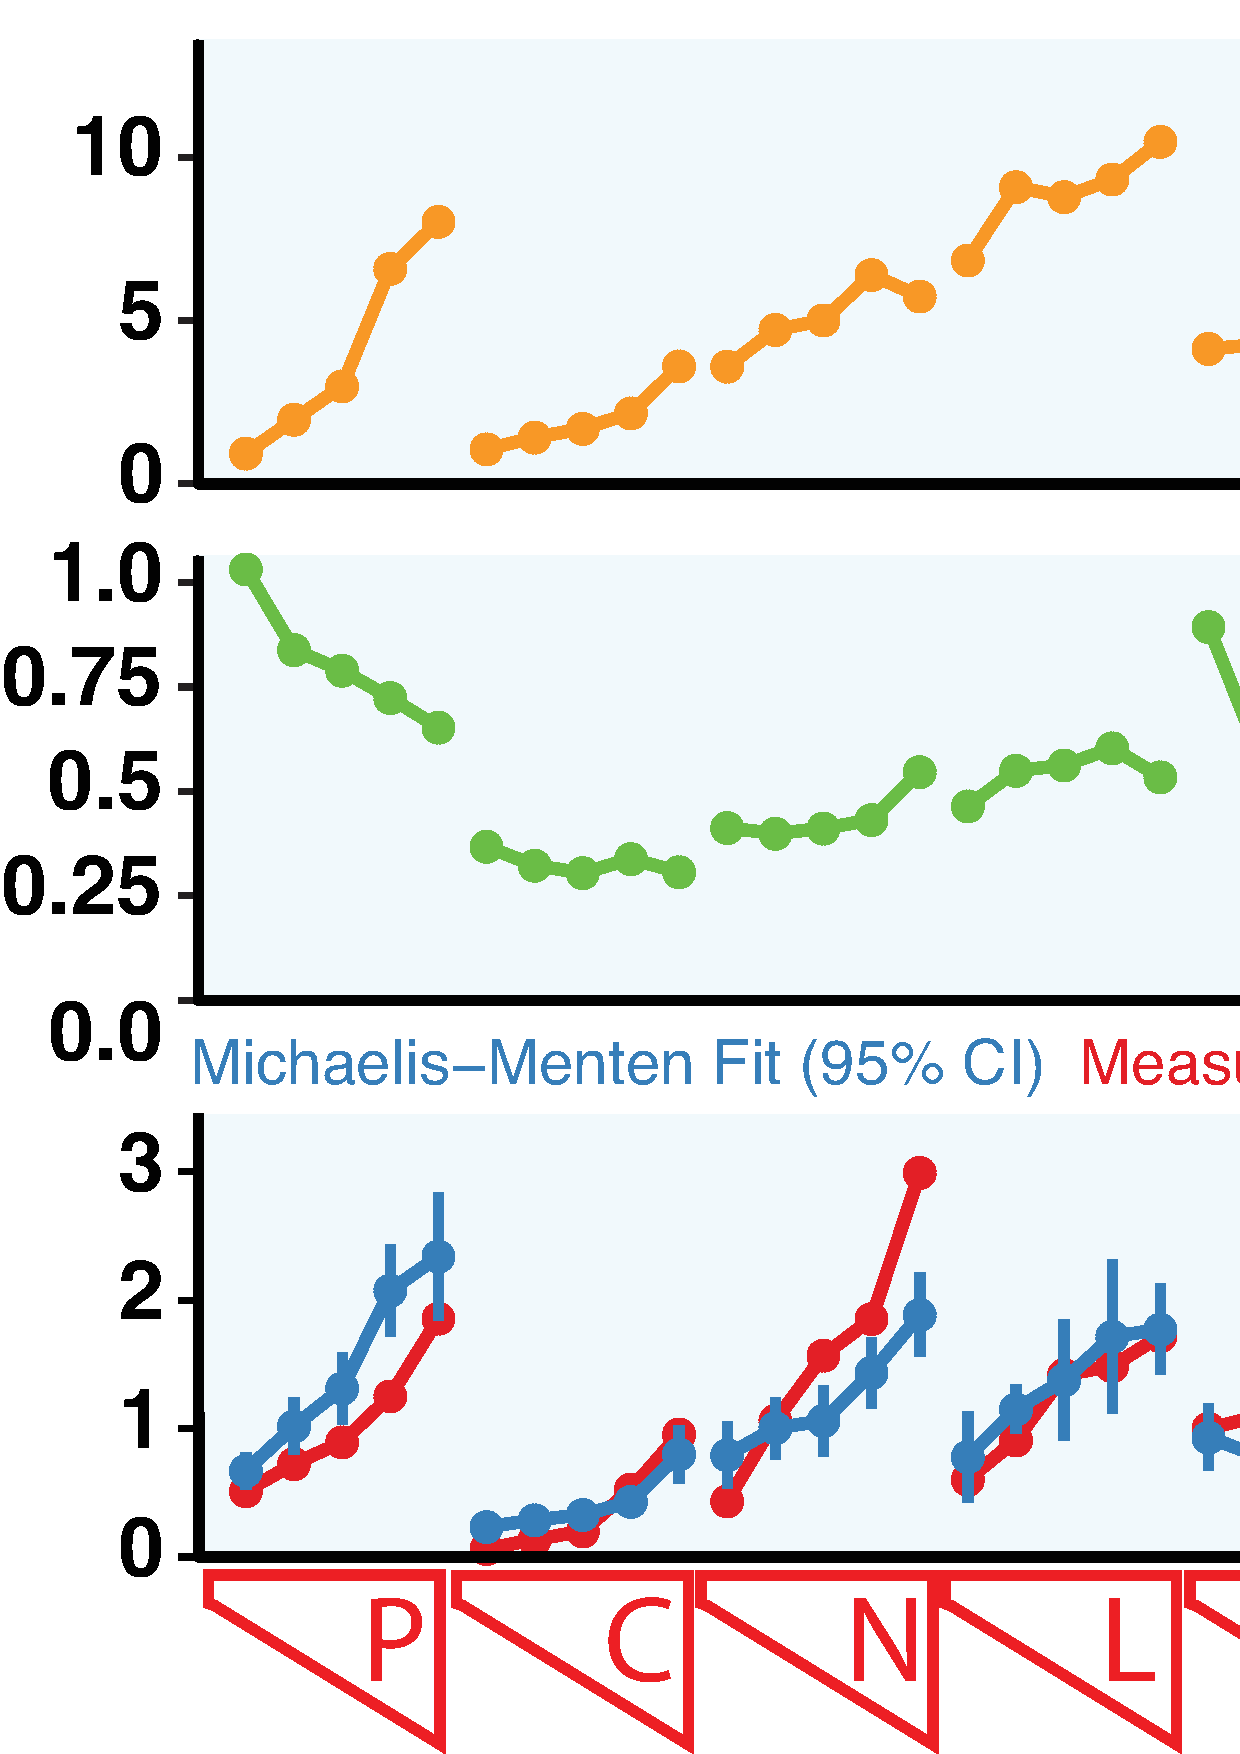
\includegraphics[width = 1\textwidth]{ch-simmer/Figures/F3-MMkinetics.pdf}
\caption[Michaelis-Menten kinetics is sufficient to relate substrate, product and enzyme concentrations to flux carried for the reaction triose-phosphate isomerase]{Michaelis-Menten kinetics is sufficient to relate substrate, product and enzyme concentrations to flux carried for the reaction triose-phosphate isomerase.  \textbf{A)} Across 25 conditions, we measured the relative concentration of the reaction substrate (DHAP: dihydroxyacetone phosphate), product (GAP: glyceraldehyde 3-phosphate) and enzyme (TPI1).  \textbf{B)} The simple Michaelis-Menten reaction form translates the 25 sets of reaction species into predict flux ($V_{rMM}$) based on the value of four inferred kinetic parameters.  Comparing measured flux to the reaction form's prediction indicates that flux through TPI can be explained by a Michaelis-Menten relationship between substrate, product and enzyme.}
\label{fig:TPI}
\end{figure}

The same approach was used to study amidophosphoribosyltransferase (ADE4), the first committed step of purine biosynthesis. Both of the substrates of this reaction were strongly influenced by limiting nutrient, with PRPP specifically depleted in phosphate limitation and glutamine in nitrogen limitation; the product glutamate was most abundant in carbon limitation (\hyperref[fig:PPAT]{Figure \ref{fig:PPAT}A}; phosphoribosylamine was not measured). Ade4p enzyme concentration was lowest in carbon limitation and greatest in leucine limitation. From these patterns of substrate, product and enzyme concentrations, it was possible to account for only half the observed variation across conditions in fluxes, which increased more with growth rate than could be accounted for based on the measured concentrations (\hyperref[fig:PPAT]{Figure \ref{fig:PPAT}B}). To determine whether allosteric regulation could rectify this inconsistency, we compiled a list of nine candidate activators and inhibitors from the BRENDA database, drawing upon both yeast-specific regulation and non-yeast regulation spanning all domains of life \cite{Scheer:2011df}. For each, the corresponding Michaelis-Menten rate law was evaluated for whether it explained the observed flux significantly better than the regulation-free rate law (q-value $<$ 0.1). Of the nine, only inhibition by adenosine monophosphate (AMP), which generally accumulates in slow growth, meaningfully improved fit (\hyperref[fig:PPAT]{Figure \ref{fig:PPAT}C}). Inhibition of the first committed step of purine biosynthesis by AMP is a logical feedback circuit that has been demonstrated in yeast and in other organisms \cite{WYNGAARDEN:1959wf, Jones:1982dn, Scheer:2011df}. Thus, from a set of candidates based on prior knowledge of metabolism, SIMMER was able to identify physiologically relevant allosteric regulation of yeast purine biosynthesis.

\begin{figure}[h!]
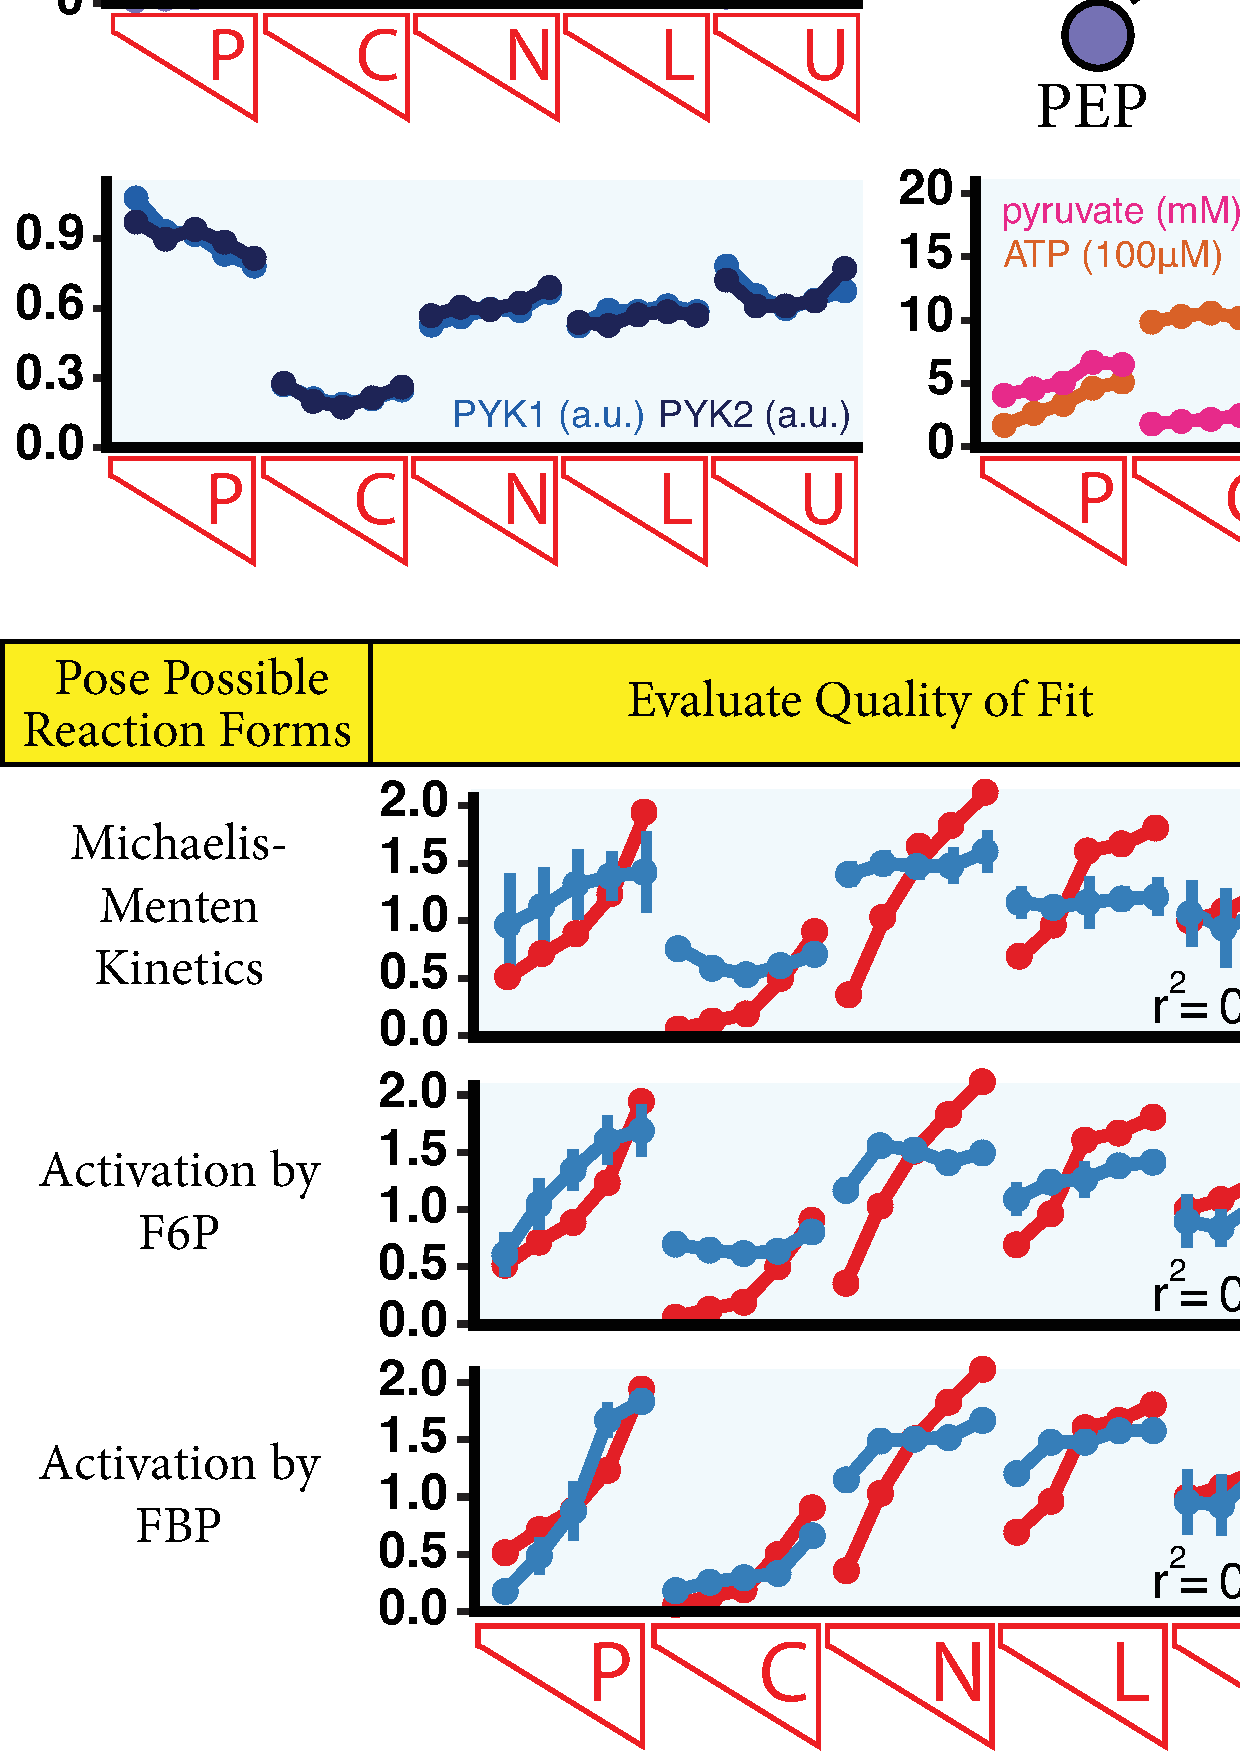
\includegraphics[width = 1\textwidth]{ch-simmer/Figures/F4-identifyingRegulation.pdf}
\caption[Two models of PRPP Amidotransferase (PPAT) kinetics are compared: reversible Michaelis-Menten kinetics with and without allosteric inhibition by AMP]{Two models of PRPP Amidotransferase (PPAT) kinetics are compared: reversible Michaelis-Menten kinetics with and without allosteric inhibition by AMP.  \textbf{A)} Across 25 conditions, we measured the relative concentrations of both substrates (PRPP:phosphoribosyl pyrophosphate and Gln:glutamine), and one product (Glu:glutamate) and the enzyme (ADE4). Unmeasured species were treated as invariant across the measured conditions. \textbf{B)} If Michaelis-Menten kinetics is approximately true \textit{in vivo}, measured flux should be a Michaelis-Menten function of substrates, products and enzymes concentrations.  While Michaelis-Menten kinetics predicts the average flux through chemostats with the same limiting nutrient, it is unable to account for increasing flux with growth-rate.  \textbf{C)} Using measured concentrations of AMP (adenosine monophosphate), treating AMP as an allosteric inhibitor results in a statistically-significant improvement in how well flux can be predicted relative to the simple Michaelis-Menten kinetics (p $<$ 3x10$^{-5}$, q $<$ 0.1).}
\label{fig:PPAT}
\end{figure}

\subsection{Strategy for combining systems-level data and prior knowledge to identify physiologically relevant regulators.}

In principle, the SIMMER approach can identify allosteric regulation without reliance on prior knowledge, by examining for each reaction whether the inclusion of each measured metabolite as an activator or inhibitor significantly improves the fit. To test this approach, we assembled an unbiased list of gold-standard physiological allosteric metabolic regulation in yeast by comprehensively summarizing existing reviews of yeast metabolic regulation \cite{Jones:1982dn, Sekine:2007ej, Fraenkel:2011wp}. Among these instances of physiological regulation, 22 regulators of 16 reactions (\hyperref[tab:GS]{Table \ref{tab:GS}}) could be tested to evaluate whether SIMMER would recapitulate this regulation. In individual testing of these 22 regulators, 45\% greatly improved the fit (p $<$ 0.01). This fraction far exceeded other reported biochemical regulators of these enzymes (22\%) or randomly selected metabolites (20\%). Testing of all possible candidates, however, produced an unwieldy number of metabolites that significant enhanced fit, whether biochemical regulators or all measured metabolites were considered (average of 3.4 and 43.4 per-reaction, respectively). This is not because each of these regulators is physiologically significant. Instead, this reflects strong correlations between the concentrations of many metabolites, such that when one improves the fit, several others also do. Moreover, this excess of predicted regulators remains after correcting for the reaction-wise false positive rate.

Because the quantitative influence of many metabolites cannot be distinguished, we focused on developing an approach that integrated knowledge from existing literature. Some biochemical characterization had been performed for each of 55 reactions for which we had complete integrative `omics data, including for the relevant Baker's yeast enzyme in 33 cases. This prior work, as summarized in the BRENDA database \cite{Scheer:2011df}, was used to assemble a list of putative regulators for each reaction. We sought to determine which of these candidate regulators, drawn from across any species, could be shown to be physiologically meaningful in yeast using SIMMER.
 
To integrate our data and prior literature knowledge, we took a Bayesian approach, aiming to maximize $Pr(Model | Data)$, where ``Model'' is a Michaelis-Menten equation including regulation and ``Model'' is ``True'' if the regulation is physiologically meaningful \cite{Gelman:2003vk}. Using Bayes Theorem, 

\begin{equation}
Pr(Model | Data) = Pr(Data | Model) Pr(Model) / Pr(Data)\label{eqtn-bayes1}
\end{equation}

$Pr(Data | Model)$ can be assessed as above based on least squares deviations between measured and predicted flux (i.e. how well concentrations predict the fluxes). $Pr(Data)$ is independent of the choice of the model, thus 

\begin{equation}
Pr(Model | Data) \propto Pr(Data | Model) Pr(Model) \label{eqtn-bayes2}
\end{equation}

To assess the \textit{a priori} probability of different models, for the 16 reactions for which we had identified gold standard regulators, we compiled a list of all known literature regulation by measured metabolites (240). We then treated the 22 instances of gold standard regulation as ``True'' models, and assessed which literature metrics might differentiate these gold standard cases. Via regression analysis, we found that the log-odds of a regulator falling in the gold standard list increased strongly with the number of regulatory annotations in BRENDA, both within yeast (p $<$ 0.002) and across non-yeast species (p $<$ 0.0002), and decreased as the total number of regulators of a reaction assessed grew (p $<$ 0.02). The resulting regression equation allows us to establish $Pr(Model)$ for any candidate regulator based on these three numerical metrics from the BRENDA database. This approach conservatively enforces that even among putative regulators listed in BRENDA, physiologically meaningful regulation is unlikely \textit{a priori} (median probability of $\sim$ 0.03), especially for well-studied reactions where the list of putative regulators is long.  


\subsection{Identification of 34 instances of physiologically meaningful yeast metabolic regulation.}

Using the above strategy, we assessed $Pr(Model | Data)$ (i.e., the probability that the regulation is physiologically significant) for each candidate literature regulator of the 56 reactions for which we had complete `omics data. For reactions where one or more regulators significantly improved fit (q-value $<$ 0.1), we tested whether cooperative binding of regulators, or the inclusion of a secondary regulator further improved fit.

By balancing the inherent plausibility of each kinetic model, $Pr(Model)$, with its quantitative support, $Pr(Data | Model)$, the model which is best supported for each reaction could be found: $Pr(Model | Data)$. For 16 reactions, we found that generalized Michaelis-Menten kinetics fit the data reasonably well (spearman correlation $>$ 0.6) and was supported over all regulatory models. We additionally identified 34 instances of physiologically-relevant regulation, including six reactions with two physiological regulators and two reactions with cooperative regulation (\hyperref[signif_regulators]{Table \ref{signif_regulators}}, \hyperref[fig:allosteryFit]{Figure \ref{fig:allosteryFit}}). 

Metabolite affinities implied by the reaction forms agree with literature estimates (\hyperref[fig:occupancy]{Figure \ref{fig:occupancy}A}) \cite{Scheer:2011df}. Substrates and products vary between unsaturated and saturated on a case-by-case basis, but regulators operate at concentrations near their affinity, where the greatest tuning of flux is possible (\hyperref[fig:occupancy]{Figure \ref{fig:occupancy}B}). Inferred thermodynamics are consistent with previous estimates of free energy drops across glycolysis (\hyperref[fig:paramaterValues]{Figure \ref{fig:paramaterValues}}) \cite{Flamholz:2013io}. For near-equilibrium reactions, there is an important role for metabolite concentrations that shift the ratio of forward to reverse flux across nutrient conditions.

The 34 instances of identified regulation encompassed five instances of ``gold standard'' yeast regulation \cite{Jones:1982dn, Sekine:2007ej, Fraenkel:2011wp}, and four regulators with strong \textit{in vitro} support in yeast \cite{Li:1996vg, Khoo:1970wt, Majtan:2014jp, VANDERCAMMEN:1989er}, but no demonstrated physiological importance. In addition to yeast-specific regulation, 22 predicted regulators had never been experimentally tested in \textit{S. cerevisiae}. Before embracing the implications of these regulatory mechanisms, we first sought to verify a subset of non-yeast regulatory \textit{in vitro}.

\begin{figure}[h!]
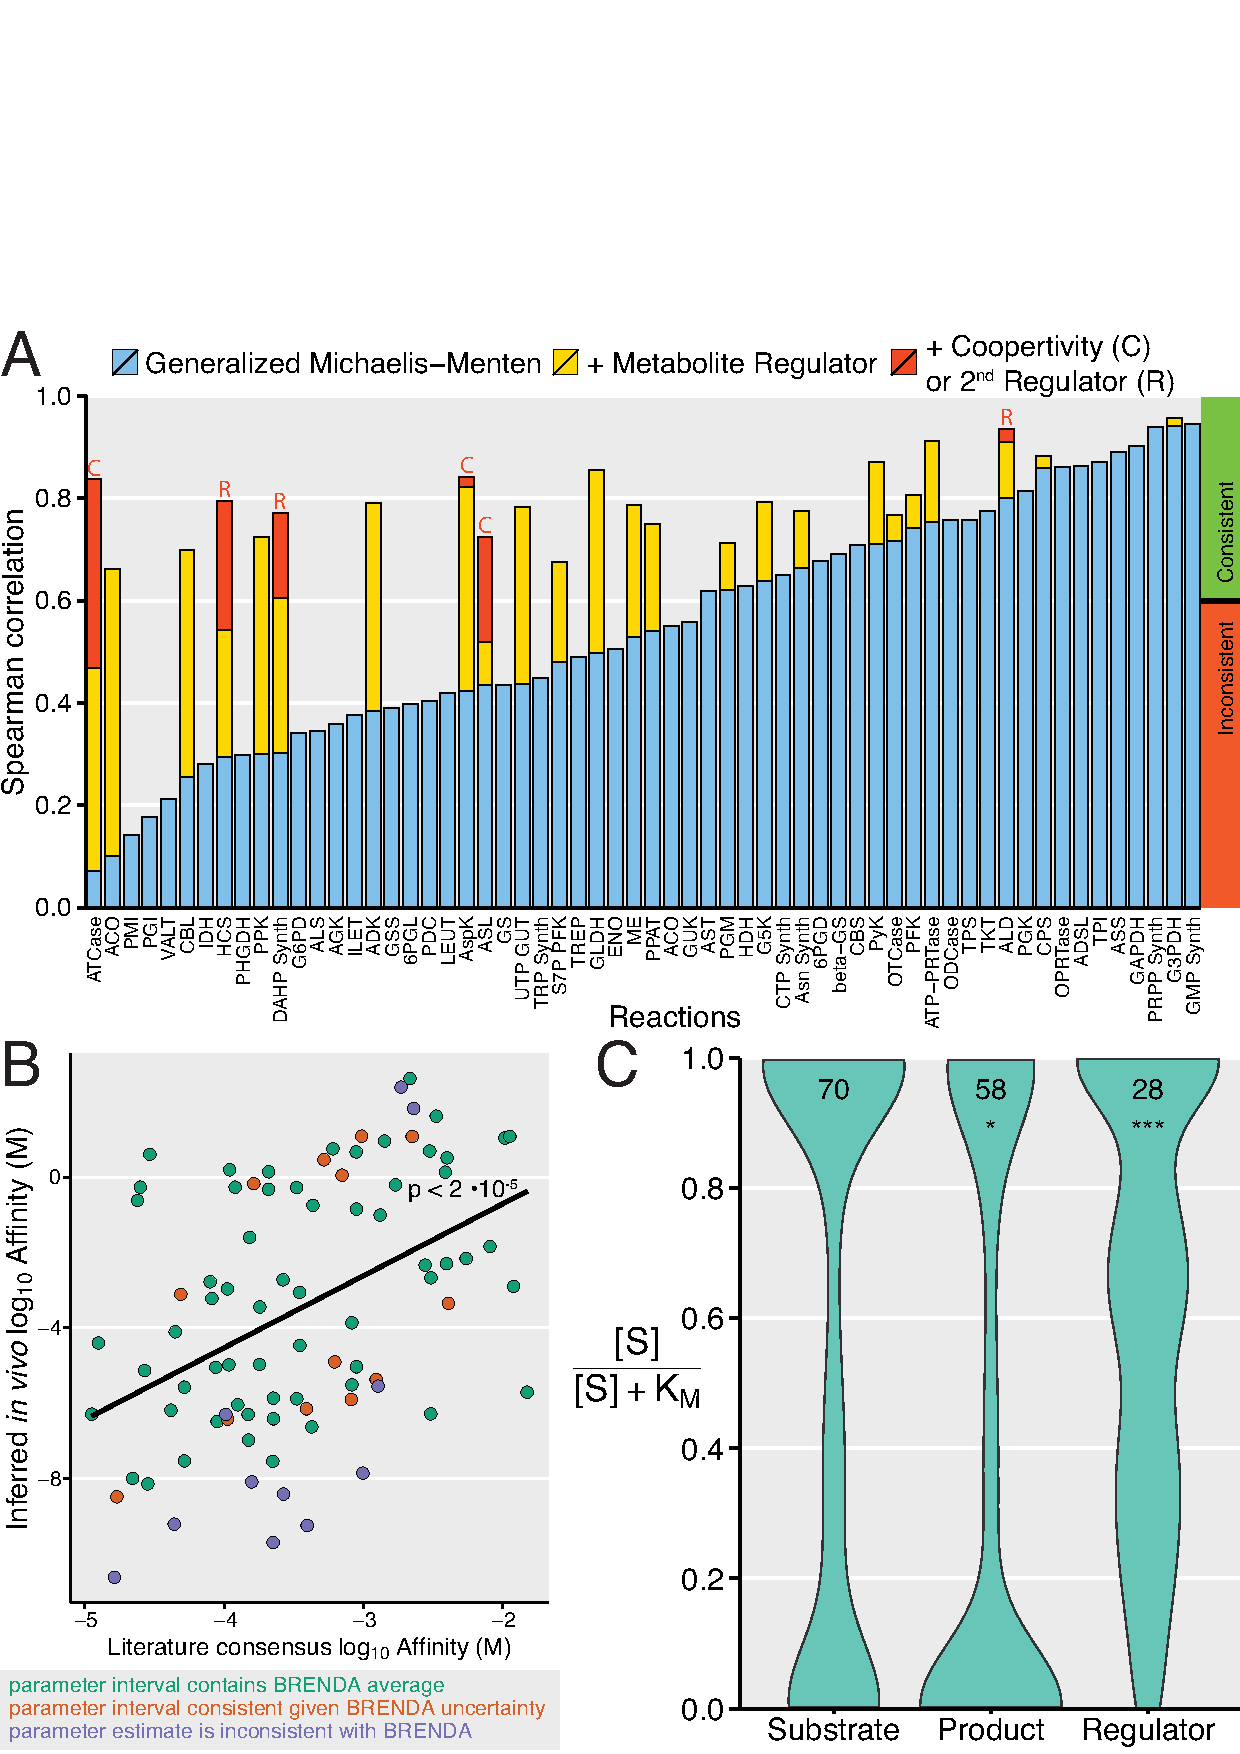
\includegraphics[width = 1\textwidth]{ch-simmer/Figures/F5-performanceSummary.pdf}
\caption[Metabolism-wide summary of the consistency between measured flux and Michaelis-Menten predictions]{Metabolism-wide summary of the consistency between measured flux and Michaelis-Menten predictions. For each of 56 reactions, the spearman correlation between measured flux and flux implied by Michaelis-Menten kinetics (with and without regulation) is shown.  For 28 reactions, inclusion of a regulator was supported, and for eight of these reactions, further improvement is possible through a secondary regulator or regulator cooperativity.  For reactions with supported regulation, the improvement in spearman correlation relative to the best-supported simpler models is shown.}
\label{fig:allosteryFit}
\end{figure}

\subsection{Evaluating \textit{in vitro} support for predicted regulation.}

To demonstrate the utility of SIMMER for computationally-guided discovery, we chose two well-studied reactions where predicted regulation departs from canon. For each reaction, precise molecular hypotheses were tested using \textit{in vitro} biochemistry.  Studying ATP-phosphoribosyltransferase (ATP-PRTase; HIS1), we found that the canonical inhibition by histidine was likely insufficient because this inhibition is strongly contingent upon ATP-PRTase's product, phosphoribosyl-ATP (\hyperref[fig:atpprtase]{Figure \ref{fig:atpprtase}}). This combinatorial regulation has previously been suggested in \textit{e. coli}, but we are the first to report its relevance in \textit{S. cerevisiae} \cite{DallLarsen:1976wm}.  Investigating ornithine transcarbamylase (OTCase; ARG3), an enzyme that is not commonly thought to be regulated through allostery \cite{Jones:1982dn}, our method predicts that alanine could serve as a physiological inhibitor.  Using both spectrophotometric and mass spectrometric assays, we confirmed that alanine inhibits Arg3p with a k$_{i}$ of 15 mM (\hyperref[fig:otcase]{Figure \ref{fig:otcase}}).  Given physiological concentrations, alanine, and to a lesser extent the other aliphatic amino acids, will differentially impact OTCase flux.  One implication of this regulation is that amino acid concentrations could indirectly stimulate ribosome synthesis, possibly allowing for a metabolic coordination of amino acid abundance and ribosome synthesis.

While we are exploring a large number of possible regulators drawn from BRENDA, these candidates still represent a small fraction of possible regulatory interactions that could exist. Identifying purely novel regulation may require checking all metabolites, but this brute force method is computationally inefficient and is also statistically unsound due to dependence between hypotheses. To deal with these challenges, we explored an alternative approach to look for purely novel regulation. Because the concentrations of possible activators and inhibitors are spanned by the metabolomic principal components, we reasoned that the trend of an optimal metabolic regulator could be found by jointly optimizing the relative abundance profile of a metabolite (via principle component loads) and the kinetic effect of this regulator (via kinetic parameters). This approach was used to identify an ``optimal'' activator and inhibitor of each reaction whose relative abundance trend could then be compared to other measured metabolites, resulting in significance rankings similar to when all metabolites are separately tested (spearman correlation, 0.44; p $<$ 1 $\times 10^{-16}$). The power of this approach is limited in this study due to model complexity but can still suggest possible regulators when either no tested reaction form is quantitatively supported or few regulatory hypotheses exist (\hyperref[fig:hypoMet]{Figure \ref{fig:hypoMet}}). Using this approach, we see that reactions with no adequate reaction form could not be rescued by an optimal regulator, suggesting some pathology greater than missing regulation, while for understudied regulation, one reaction, guanylate kinase (GUK1), showed evidence of regulation.

\subsection{Assessing how metabolites and enzymes change flux.}

In order to reach a clean alignment of measured flux and a kinetic model's prediction, this model implicitly accounts for the extent of concentration variability for each reaction specie and the impact of this variation on flux.  Not all reaction species are equally important in this regard; some species may remain at nearly fixed concentration or changes in their concentration may not change flux (e.g. saturated metabolites or minor isoenzymes).  To understand which species are important in driving variable flux through each reaction, we need a quantitative way to dissect the combined role of all species in driving variable flux into the marginal contribution of each metabolite and enzyme.  A specie's role in driving variable flux is related to two factors: the magnitude by which a specie's concentration varies and the way in which flux through the reaction responds to changes in this specie's concentration.  The influence of a single specie, its \textit{metabolic leverage}, is roughly proportional to the product of its fold-change and average elasticity $\left(\epsilon = \frac{\partial J}{\partial S}\frac{[S]}{J}\right)$ \cite{Kacser:1973fe, Liao:1993in}.

Calculating metabolic leverage for each of the 44 well-fit reactions, allows us to determine how the total variable flux in these reactions has resulted from changes of reaction species.  Summarizing the relative influence of substrates, products, enzymes and regulators (\hyperref[fig:metabolicLeverage]{Figure \ref{fig:metabolicLeverage}}, \hyperref[fig:MLbar]{Figure \ref{fig:MLbar}}), we see that reversible reactions are almost entirely driven by changes in substrate and product concentrations, although the relative influence of substrates and products varies from reaction to reaction.  In contrast, irreversible reactions are driven primarily by substrate and enzyme concentrations; and for select reactions, regulators also have an important role. In the vast majority of cases, even when strong regulation exists, a single regulator rarely dominates. Instead, flux is collectively dictated by substrates, enzymes and regulators.

\begin{figure}[H]
\floatbox[{\capbeside\thisfloatsetup{capbesideposition={right,top},capbesidewidth=6cm}}]{figure}[\FBwidth]
{\caption[Flux changes in response to changing concentrations of metabolites and enzymes whose impact on flux is governed by the metabolite and enzyme elasticity]{\fixedspaceword{Flux changes in response to changing concentrations of metabolites and enzymes whose impact on flux is governed by the metabolite and enzyme elasticity.  The impact of a single metabolite or enzyme in driving variable flux is roughly proportional to its elasticity weighted by the standard deviation of log relative concentrations across physiological conditions (phosphate, carbon and nitrogen limitations).  For a reaction, the relative contributions of its enzymes, substrates and regulators in driving variable flux across physiological conditions can be approximated by this metabolic leverage.  \textbf{A)} Metabolic leverage can be projected onto a ternary surface where each reaction is affected by enzymes, substrates, products, and possibly regulators whose influence sums to 100\% leverage.  \textbf{B)} This metric is able to distinguish reactions that are irreversible and thus likely to be good points of regulation from more passive reversible reactions. Reactions are classified as kinetically irreversible if literature suggests that net flux only proceeds in the forward direction \cite{Heavner:2012dg}. \textbf{C)} Pie chart summary of average metabolic leverage for irreversible and reversible reactions.
}}\label{fig:metabolicLeverage}}
{\includegraphics[width=\textwidth-6cm]{ch-simmer/Figures/F6-MetabolicLeverage.pdf}}
\end{figure}

When reactions respond strongly to changes in enzyme or regulator concentrations, it is likely that these regulatory events causally change flux or metabolite concentrations.  We can test this assertion, which links metabolic leverage to metabolic control, by studying glycolysis where reaction kinetics are well-fit, allowing a comparison of reaction-level and pathway-level inference.  Using the optimal reaction forms for glycolytic reactions, two metabolic control analysis (MCA) models of glycolysis were created which contrast the metabolic consequences of two similarly supported regulatory mechanisms for pyruvate kinase \cite{Cortassa:1994is, Westerhoff:1987jo}. This model reproduces the finding that glycolytic flux is predominately governed by phosphofructokinase (PFK; PFK1,2) \cite{Cortassa:1994is}, while the feed-forward regulation on pyruvate kinase (PyK; CDC19, PYK2) by fructose 1,6-bisphosphate primarily changes metabolite concentrations rather than flux per se, in line with experimental findings \cite{Xu:2012gg} (\hyperref[fig:MCA]{Figure \ref{fig:MCA}}). Projecting metabolic leverage onto a metabolic map (\hyperref[fig:MLpathways]{Figure \ref{fig:MLpathways}}), it is clear that phosphofructokinase and pyruvate kinase are the most important regulatory reactions in glycolysis.  This agreement suggests that metabolic leverage can provide a first-glance at the control of pathways (\hyperref[fig:MLpathways]{Figure \ref{fig:MLpathways}}) when comprehensive analysis using MCA is not immediately possible.  For instance, production of structural glucans is governed by the concentration of the beta-glucan synthases (FKS1, GSC2), while the production of aspartate family amino acids, as well as the interconversion of purines and pyrimidines operates without external regulation; instead, flux is driven solely by changes in substrate and product concentrations. 

\section{Discussion}

As we move from understanding the behavior of individual metabolic pathways to understanding metabolism as a complete system, there is a pressing need for methods that excel at these larger scales. Previous attempts to infer metabolic regulation have evaluated model support at a systems-level.  This has forced researchers either to use strong \textit{a priori} assumptions about how metabolism functions (and thereby only explore a small amount of hypothesis space) \cite{Chassagnole:2002ty, Zampar:2013fr} or to restrict their focus to relatively small metabolic networks that could be comprehensively interrogated \cite{Link:2013dj}, albeit with poor scaling ($\mathcal{O}(n^{m})$ for $n$ reactions and $m$ possible reactions forms of each reaction). By measuring flux, rather than inferring it based on changing metabolite concentrations, reactions can be rendered independent, and metabolism can be studied on a reaction-by-reaction basis. When this approach is adopted, metabolic inference scales linearly with the number of reactions and the number of regulators we want to consider for each reaction ($\mathcal{O}(nm)$). Furthermore, each reaction-level model can be evaluated more quickly than metabolism-level models, and correct models of individual reactions can be found without necessitating that the kinetics of all reactions be correct. In our study, we used this approach to push beyond pathway-level analysis to investigate metabolic regulation at the level of complete metabolism. We addressed two outstanding challenges in chemical biology: how to systematically identify physiological regulation that may be entirely novel and whether `omic data can elucidate the physiological control of flux.

These topics are extremely important in microbial metabolic engineering, where researchers frequently attempt to preferentially direct flux through pathways of interest.  Because microbial metabolism has evolved chiefly to exhibit robustness, native regulation ingrained in the metabolic network is frequently at odds with design goals \cite{Kitano:2007cp}.  As such, pathway engineering efforts are frequently hampered when cryptic metabolic regulation exists or the relationship between pathway fluxes and enzyme abundance is unclear.  Using SIMMER, solutions to both challenges can be found.  When a native allosteric regulator is important, this regulation can be identified based on its physiological impact, allowing targeted experiments to abolish the regulators binding. To determine how enzyme levels should be tweaked to alter pathway flux, we hypothesize that by mimicking physiological control mechanisms for select reactions where flux strongly tracks enzyme abundance, over-expressing enzymes will result in changes in flux.  Our analysis suggests that such examples are rare, paralleling experimental observations that pathway fluxes are rarely limited by the expression of a single enzyme \cite{Hauf:2000vu, CornishBowden:1995fy}.  For such pathways where flux depends on multiple reactions, we have demonstrated, using glycolysis as an example, that the physiological reaction forms which we have inferred can be coupled together to provide a more accurate characterization of pathway control.

In this study, we have focused on characterizing the metabolism of \textit{S. cerevisiae}, a microbe whose metabolism is relatively well understood; but, our approach can be applied to any organism that can be grown in suspension in which metabolic behavior can be varied using either nutritional or genetic perturbations.  We feel that this approach will be particularly useful for providing a preliminary understanding of lesser understood organisms, where traditional approaches based on studying one enzyme at a time, are intractable.  Beyond providing such a one-shot characterization of metabolism, most lesser-studied organisms will contain reactions which have been scarcely biochemically characterized.  We have provided solutions for identifying regulation using little prior literature knowledge by either capitalizing upon regulatory conservation or searching for purely novel regulation by an optimum regulator.

While our data is the most comprehensive enzyme-metabolite-flux dataset to date, it is still not a complete collection of all relevant metabolic information.  Fulfilling the promise of SIMMER will require both progressively refining our input data and expanding the breadth of our analysis.  Improving our current data will largely depend upon improving the number of distinct metabolites that can be measured through metabolomics and improving the accuracy of flux determination.  Here, advances in instrumentation paired with more focused analytical methods should afford both a more accurate and comprehensive detection of relevant metabolites. The use of stable isotope labeling could further improve flux accuracy \cite{Yuan:2008er}.

Expanding the breadth of our dataset will entail addressing biological phenomena that were beyond the scope of this study.  Chiefly, we are unable to assess the extent to which flux is impacted by post-translational regulation \cite{Fiedler:2009hx, Schulz:2014eo}, variable sub-cellular localization \cite{Kitamoto:1988wc} or cell-to-cell variability \cite{Tu:2005cv}.  These limitations are likely to blame for the 12 reactions where no adequate kinetic model could be found, although inaccurate measurements or missing regulation could also result in inappropriate regulatory predictions that partially compensate for unmeasured factors.  A final issue of note is that we had to make assumptions about the form of rate laws, and while true \textit{in vivo} rate laws rarely reduce to generalized Michaelis-Menten kinetics \cite{Hill:1977vm}, our reaction forms are able to achieve an approximately correct relationship between species and resulting flux across the physiological conditions investigated. Thus, these simplified kinetics are functionally sufficient for our purposes \cite{Fell:1997wg}.

Because we have characterized a reproducible set of conditions that contain much of the meaningful metabolic variation in yeast, we hope that this study will serve as an important scaffold for future work to build upon, whether by incorporating additional experimental information on existing conditions or by expanding the breadth of the study by characterizing additional conditions. Regulation can only be identified if it differentially impacts study conditions. By expanding the number of conditions that are investigated, we can unmask regulation that is important in these conditions. Our approach can identify this regulation by virtue of the kinetic importance it gains in these new conditions. This will also serve to refine the accuracy of parameter estimates from reaction forms and better discriminate  competing regulatory hypotheses.

\section{Supplemental figures and tables}

\setcounter{figure}{0}
\makeatletter 
\renewcommand{\thefigure}{\thechapter.S\@arabic\c@figure}
\renewcommand{\thetable}{\thechapter.S\@arabic\c@table}
\renewcommand{\theequation}{\thechapter.S\@arabic\c@equation}
\makeatother



\begin{figure}[H]
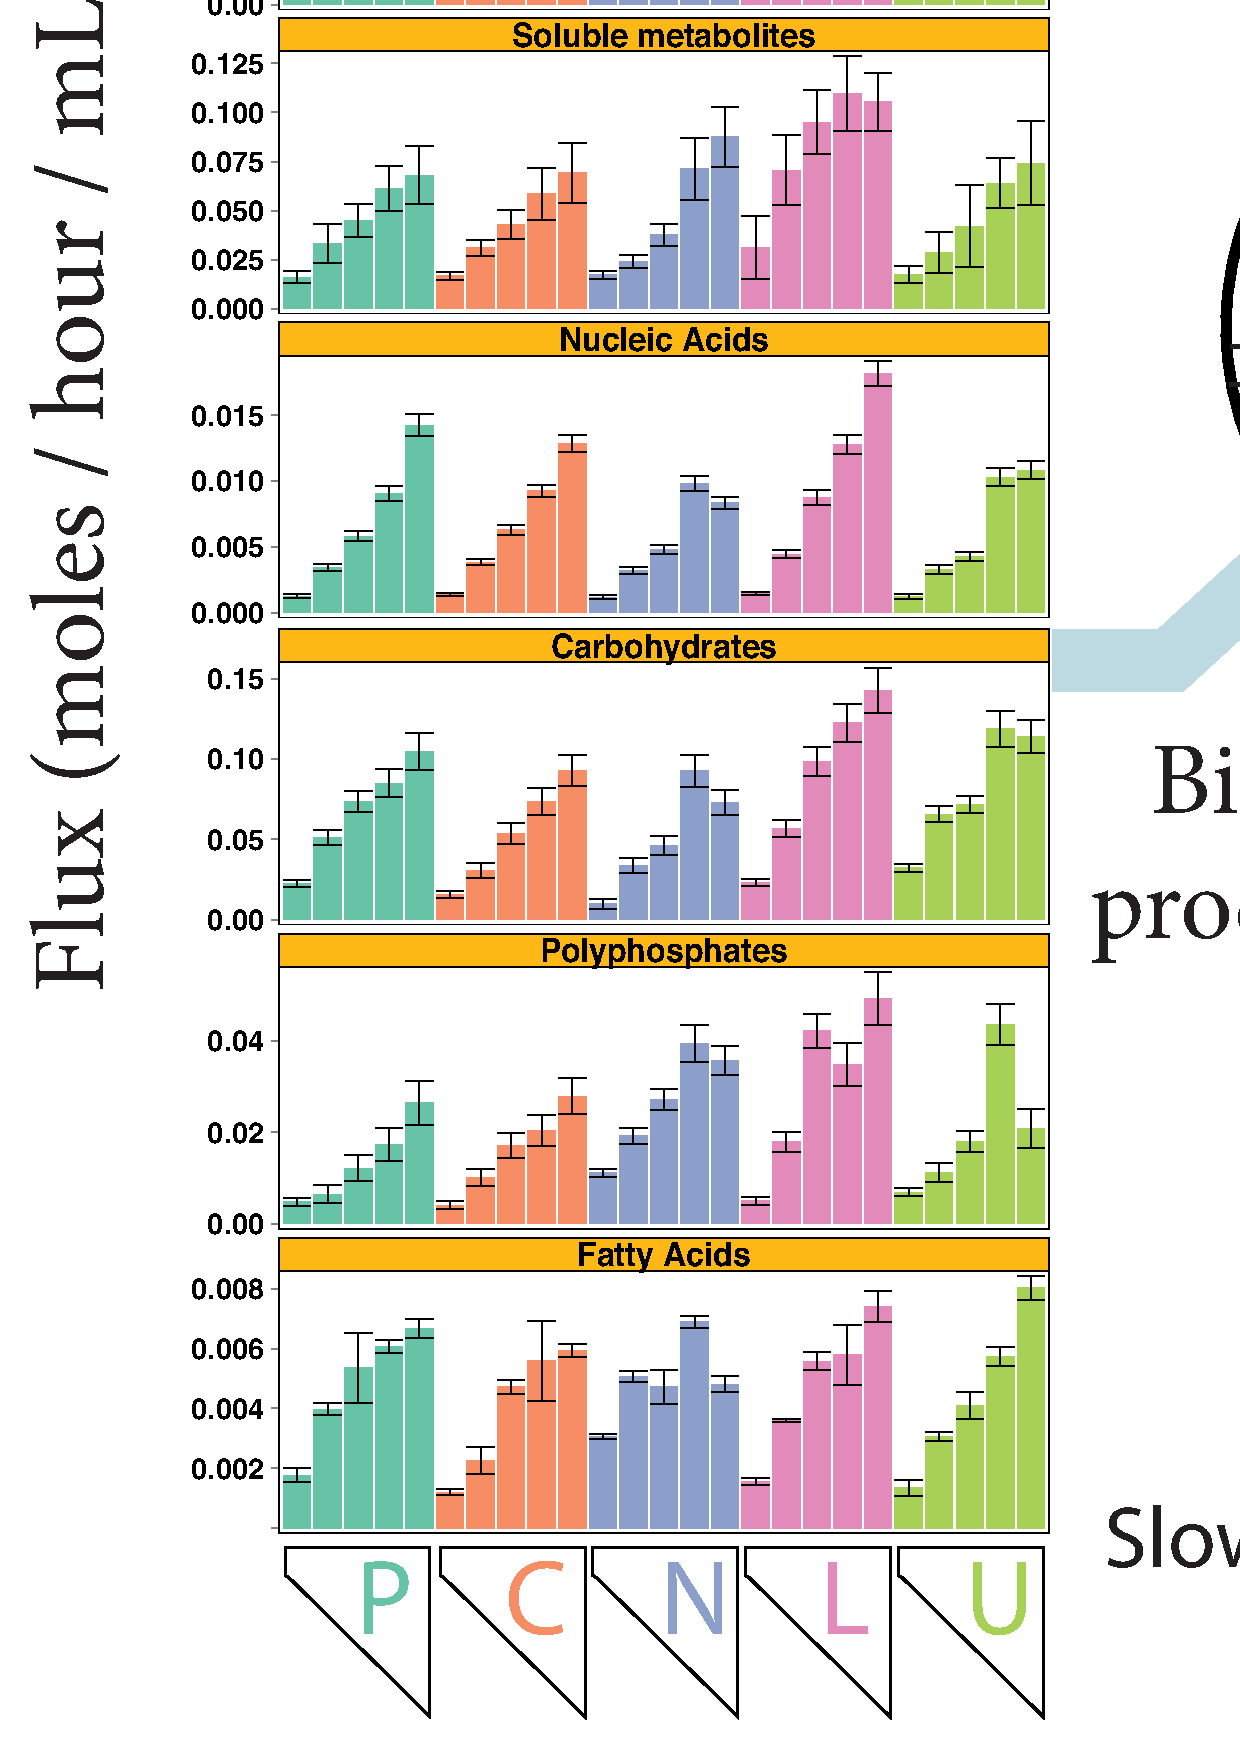
\includegraphics[width = 0.8\textwidth]{ch-simmer/Figures/Supplement/boundaryFluxes.pdf}
\caption[Summary of experimentally-determined rates of metabolite uptake, excretion and incorporation into biomass for each chemostat condition]{Summary of experimentally-determined rates of metabolite uptake, excretion and incorporation into biomass for each chemostat condition.}
\label{fig:boundFlux}
\end{figure}

\begin{figure}[H]
\includegraphics[width = 0.7\textwidth]{ch-simmer/Figures/Supplement/fluxHM.pdf}
\caption[Heatmap summarizing relative flux through 233 reactions across chemostat conditions]{Heatmap summarizing relative flux through 233 reactions across chemostat conditions.  Absolute reactions fluxes were determined independently for each chemostat. To visualize reactions whose flux was correlated, the flux through each reaction was expressed relative to the median absolute flux across all conditions.  Reactions were organized using hierarchical clustering using absolute pearson correlation with average linkage.  Only reactions that were well-constrained based on flux variability analysis are shown.}
\label{fig:fluxHM}
\end{figure}

\begin{figure}[H]
\includegraphics[width = 0.5\textwidth]{ch-simmer/Figures/Supplement/peptide_RA_reproduce.pdf}
\caption[Nutrient-induced changes in peptide abundance between technical replicates are highly reproducible]{Nutrient-induced changes in peptide abundance between technical replicates are highly reproducible.  As a representative example, a slow growth nitrogen-limited chemostat (n0.05) is compared to an internal reference slow-growth phosphorous-limited $^{15}$N-labelled chemostat ($^{15}N$-p0.05).  For each of two technical replicates derived from independent digestion, fractionation and mass spectrometry of a single sample, the relative abundance of unlabelled experimental peptides relative to $^{15}N$-labelled reference peptides is shown.}
\label{fig:proteomicsConsistency}
\end{figure}

\begin{figure}[H]
\includegraphics[width = 0.7\textwidth]{ch-simmer/Figures/Supplement/proteinHM.pdf}
\caption[Heatmap summarizing the variable concentration of 1,187 proteins across chemostat conditions]{Heatmap summarizing the variable concentration of 1,187 proteins across chemostat conditions. From the ratio of unlabelled sample peptides to matching $^{15}N$-labelled reference peptides, the abundance of each enzyme relative to a common reference was determined.  Across the 25 conditions, protein relative abundances were mean-centered, log-transformed and organized by hierarchical clustering using pearson correlation with average linkage.}
\label{fig:proteinHM}
\end{figure}

\newcommand{\multilineR}[1]{\begin{tabular}[b]{@{}r@{}}#1\end{tabular}}
\newcommand{\multilineL}[1]{\begin{tabular}[b]{@{}l@{}}#1\end{tabular}}
\newcommand{\multilineC}[1]{\begin{tabular}[b]{@{}c@{}}#1\end{tabular}}

\newcolumntype{L}[1]{>{\raggedright\let\newline\\\arraybackslash\hspace{0pt}}m{#1}}
\newcolumntype{C}[1]{>{\centering\let\newline\\\arraybackslash\hspace{0pt}}m{#1}}
\newcolumntype{R}[1]{>{\raggedleft\let\newline\\\arraybackslash\hspace{0pt}}m{#1}}

\begin{singlespace}
\begin{table}[H]
\centering
\begin{tabular}{l>{\hfill}p{0.5in}>{\hfill}p{0.5in}>{\hfill}p{0.5in}>{\hfill}p{0.5in}>{\hfill}p{0.5in}>{\hfill}p{0.5in}}
 \begin{sideways} \begin{turn}{-90}\textbf{Pathway}\end{turn} \end{sideways} & \begin{sideways} \multilineL{Reactions with\\measured enzymes} \end{sideways} & \begin{sideways} \multilineL{Total pathway\\reactions} \end{sideways} & \begin{sideways} \multilineL{Fraction of reactions\\with measured enzymes} \end{sideways} & \begin{sideways} \multilineL{Measured enzymes} \end{sideways} & \begin{sideways} \multilineL{Total enzymes} \end{sideways} & \begin{sideways} \multilineL{Fraction of\\measured enzymes} \end{sideways} \\ 
  \hline
\multicolumn{1}{l||}{Glycolysis / Gluconeogenesis} &  16 &  16 & 100\% &  17 &  18 & 94\% \\ 
  \multicolumn{1}{l||}{Citrate cycle (TCA cycle)} &  12 &  12 & 100\% &  12 &  12 & 100\% \\ 
  \multicolumn{1}{l||}{Biosynthesis of amino acids} &  73 &  83 & 88\% &  63 &  75 & 84\% \\ 
  \multicolumn{1}{l||}{Purine metabolism} &  37 &  52 & 71\% &  28 &  41 & 68\% \\ 
  \multicolumn{1}{l||}{Pyrimidine metabolism} &  27 &  39 & 69\% &  22 &  31 & 71\% \\ 
  \multicolumn{1}{l||}{All reactions} & 346 & 524 & 66\% & 304 & 510 & 60\% \\ 
   \hline
\end{tabular}
\caption[For major metabolic pathways, the coverage of enzymes measured through proteomics is summarized]{For major metabolic pathways, the coverage of enzymes measured through proteomics is summarized.  For each pathway, we show both the the fraction of reactions where at least one enzyme was measured, as well as the total fraction of enzymes measured.  Pathway annotation are based on KEGG.}
\label{protTable}
\end{table}
\end{singlespace}

\footnotesize
\begin{singlespace}
\begin{table}[H]
\centering
\begin{tabular}{|l|l|l|}
\hline
Reaction Name & Regulation & Support \\\Xhline{2\arrayrulewidth} 
3-phosphoglycerate dehydrogenase & (-) Serine & \textcolor{BurntOrange}{Alternative regulation supported}\\\hline
\multirow{2}{*}{Acetolactate synthase} & (+) ATP & \textcolor{ForestGreen}{Strongest support}\\ 
  & (-) Valine & Other GS supported\\\hline
 Acetylglutamate kinase & (-) Arginine & \textcolor{BurntOrange}{No tested model is adequate}\\\hline 
 Asparagine synthetase & (-) Asparagine & \textcolor{Cerulean}{No physiological regulation}\\\hline 
 Aspartate carbamoyltransferase & (-) UTP & \textcolor{BurntOrange}{Alternative regulation supported}\\\hline 
 \multirow{2}{*}{Aspartokinase} & (-) Homoserine & \textcolor{LimeGreen}{Supported}\\ 
  & (-) Threonine & \textcolor{ForestGreen}{Strongest support}\\\hline 
 ATP phosphoribosyltransferase & (-) Histidine & \textcolor{LimeGreen}{Supported}\\\hline 
 Carbamoyl phosphate synthase & (-) UTP & \textcolor{Cerulean}{No physiological regulation}\\\hline 
 CTP synthase & (-) CTP & \textcolor{BurntOrange}{No tested model is adequate}\\\hline 
 \multirow{2}{*}{DAHP synthase} & (-) Phenylalanine & \textcolor{LimeGreen}{Supported}\\ 
  & (-) Tyrosine & \textcolor{LimeGreen}{Supported}\\\hline 
 Glutamate 5-kinase & (-) Proline & \textcolor{ForestGreen}{Strongest support}\\\hline 
 Homocitrate synthase & (-) Lysine & \textcolor{ForestGreen}{Strongest support}\\\hline 
 Homoserine kinase & (-) Threonine & \textcolor{BurntOrange}{No tested model is adequate}\\\hline 
 \multirow{3}{*}{Phosphofructokinase} & (+) AMP & \textcolor{BurntOrange}{Alternative regulation supported}\\ 
  & (-) ATP & \textcolor{BurntOrange}{Alternative regulation supported}\\ 
  & (+) Fructose 2,6-P$_{2}$ & Not measured\\\hline 
 PRPP amidotransferase & (-) AMP & \textcolor{ForestGreen}{Strongest support}\\\hline 
 \multirow{4}{*}{Pyruvate kinase} & (-) ATP & Other GS supported\\ 
 & (+) Ammonia & Not measured\\ 
 & (-) Citrate & \textcolor{LimeGreen}{Supported}\\ 
 & (+) Fructose 1,6-P$_{2}$ & \textcolor{LimeGreen}{Supported}\\ 
   \hline
\end{tabular}
\caption[Gold-standard yeast metabolic regulation]{Gold-standard yeast metabolic regulation.  Previous analysis of 16 reactions in yeast has strongly implicated a role for 24 catalytically important regulators.  22 of these 24 regulatory relationships could be tested using the SIMMER methodology. \textcolor{ForestGreen}{Strongest support}, indicates gold standard regulation that was predicted as the best candidate physiological regulator. \textcolor{LimeGreen}{Supported}, indicates regulator's which improved fit, but were not as strongly supported as alternative literature hypotheses. \textcolor{Cerulean}{No physiological regulation}, indicates that Michaelis-Menten kinetics was supported over all literature candidates. \textcolor{BurntOrange}{Alternative regulation supported}, indicates that the tested mechanism did not meaningfully improve Michaelis-Menten kinetics, but alternative literature hypotheses were supported. \textcolor{BurntOrange}{No tested model is adequate}, indicates that among all tested regulators, none were supported.}
\label{tab:GS}
\end{table}
\end{singlespace}
\normalsize


\footnotesize
\begin{singlespace}
\begin{sidewaystable}
\centering
\caption[34 Predicted physiological regulators of yeast metabolism]{34 Predicted physiological regulators of yeast metabolism}
\label{signif_regulators}
\begin{tabular}{|l l || r r| r l|}\hline
&&\multicolumn{2}{c|}{Citations}&&\\
Reaction&Regulator&S. cer&Other&Prior Rank&Class\\\Xhline{2\arrayrulewidth} 
Acetolactate Synthase&(+) ATP&1&0&4 of 6&GS\\
Aspartate Kinase&(-) Threonine&7&34&1 of 18&GS\\
Glutamate 5-Kinase&(-) Proline&1&23&1 of 4&GS\\
Homocitrate Synthase&(-) Lysine&8&18&1 of 9&GS\\
PRPP Amidotransferase&(-) AMP&1&20&1 of 9&GS\\
Adenylate Kinase&(-) AMP&1&15&1 of 18&Sensible\\
Cystathionine Beta-Synthase&(+) SAM&2&20&1 of 5&Sensible\\
Guanylate Kinase&(-) GMP&5&2&1 of 3&Sensible\\
Trehalose-phosphate Synthase&(-) Inorganic Phosphate&4&4&1 of 4&Sensible\\
Homocitrate Synthase&(-) Quinolinate&1&0&3 of 9&Unlikely\\
Aldolase&(-) AMP&1&75&1 of 31&Pathological\\
Phosphoglycerate Mutase&(-) 3-Phosphoglycerate&1&2&1 of 4&Pathological\\\hline
Ornithine Carbamoyltransferase&(-) Alanine&0&4&6 of 27&Biochemically validated\\
Glucose 6-phosphate Dehydrogenase&(-) AMP&0&3&6 of 14&Sensible\\
Pyruvate Kinase&(-) Isocitrate&0&7&13 of 44&Sensible\\
Trehalose-phosphatase&(+) F6P&0&1&6 of 7&Sensible\\
UTP G1P Uridyltransferase&(-) UDP-Glucose&0&11&1 of 8&Sensible\\
Adenylate Kinase&(+) Threonine&0&1&17 of 18&Unlikely\\
Cystathionine Gamma-lyase&(-) Alanine&0&2&2 of 6&Unlikely\\
DAHP Synthase&(-) PEP&0&2&10 of 11&Unlikely\\
Glucose 6-phosphate Dehydrogenase&(-) PEP&0&3&8 of 14&Unlikely\\
Glutamate Dehydrogenase (NADP)&(-) Quinolinate&0&4&25 of 49&Unlikely\\
Malic Enzyme (NAD)&(-) AMP&0&4&10 of 32&Unlikely\\
Phosphofructokinase&(-) AMP&0&11&11 of 27&Unlikely\\
Phosphogluconate Dehydrogenase&(+) Aspartate&0&1&16 of 18&Unlikely\\
Phosphoglycerate Dehydrogenase&(+) Methionine&0&1&9 of 10&Unlikely\\
Pyruvate Decarboxylase&(-) Phenylpyruvate&0&2&4 of 4&Unlikely\\
Pyruvate Kinase&(-) AMP&0&7&12 of 44&Unlikely\\
ATP-Phosphoribosyltransferase&(-) AMP&0&4&2 of 4&Biochemically invalidated\\
DAHP Synthase&(-) Phenylpyruvate&0&3&8 of 11&Biochemically invalidated\\
Aspartate Carbamoyltransferase&(+) UTP&0&2&28 of 33&Pathological\\
Citrate to Cis-aconitate&(-) Isocitrate&0&2&9 of 9&Pathological\\
S7P Phosphofructokinase&(-) Phosphoenolpyruvate&0&29&7 of 27&Pathological\\
Trehalose-phosphatase&(+) Trehalose&0&1&7 of 7&Pathological\\\hline
\end{tabular}
\end{sidewaystable}
\end{singlespace}

\begin{figure}[H]
\includegraphics[width = 0.9\textwidth]{ch-simmer/Figures/Supplement/performanceSummary.pdf}
\caption[Predicted metabolite affinities are consistent with literature reports and reveal different trends in occupancy for substrates, products and regulators]{Predicted metabolite affinities are consistent with literature reports and reveal different trends in occupancy for substrates, products and regulators. \textbf{A)} Using the best-fit reaction forms, the affinity of substrates and products with measured absolute concentrations were compared to metabolite affinities found in BRENDA.  For 73\% of metabolites, the parameter 95\% CI contains the literature consensus affinity (mean of log$_{10}$ affinities), while for 89\% of metabolites, the 95\% CI overlaps the sampling distribution of literature estimates (mean $\pm 2 \cdot \sigma$(log$_{10}$ affinities). \textbf{B)} Using the best-fit reaction forms, occupancies implied by the maximum likelihood (ML) estimate of affinities for every measured substrate, product and regulator were compared. The shown violin plot was generated using one occupancy value for each metabolite's affinity for an enzyme in every condition.  To determine if this pattern differed between substrates, products and regulators, for each class, median relative affinity ML estimates formed an empirical distribution that could be compared to the log-uniform expectation using a KS test (* p $<$ 0.05; *** p $<$ 0.001). The number of metabolite-enzyme affinities used for each class is listed.}
\label{fig:occupancy}
\end{figure}

\begin{figure}[H]
\includegraphics[width = 0.9\textwidth]{ch-simmer/Figures/Supplement/parameterSummary.pdf}
\caption[Predicted reaction thermodynamics are consistent with reported literature]{Predicted reaction thermodynamics are consistent with reported literature. \textbf{A)} Demonstrating parameter estimates using Triose-phosphate isomerase with reversible Michaelis-Menten kinetics as an example.  Affinity parameters are varied relative to the median metabolite concentration and K$_{eq}$ is determined relative to the median reaction quotient (Q), giving the disequilibrium ratio ($\rho = \sfrac{Q}{K_{eq}}$).  The value of each parameter is summarized by the maximum likelihood (ML) estimator and by the 95\% credibility interval (CI).  The lower hinge of the median disequilibrium ratio specifies the minimal permissible disequilbrium needed for approximately correct prediction.  \textbf{B)} Using the best-fit reaction forms, the ML estimate of median disequilbirium (blue circle) and minimal permissible disequilbirium (black cross-bar) are shown.  To visualize how disequilbirium changes across conditions, the density of reaction quotients for each condition is shown about the minimal permissible disequilbrium; for reactions where the ML estimate is near the minimal permissible disequilibrium this variation in disequilibrium is kinetically important.  To compare inferred disequilbirium to literature reports, the disequilbrium in fast-growth carbon-limited chemostat (green circle) can be compared to findings from batch-culture.  Looking at glycolysis, we see that this approach accurately predicts that the steps with the greatest disequilbirium are phosphofructokinase and pyruvate kinase, while steps that are closer to equilibrium, phosphoglycerate kinase, phosphoglycerate mutase, aldolase and triose-phosphate isomerase, are highly reversible.}
\label{fig:paramaterValues}
\end{figure}

\begin{figure}[H]
\includegraphics[width = 1\textwidth]{ch-simmer/Figures/Supplement/HIStimecourse.pdf}
\caption[Inhibition of His1p by histidine is contingent upon the reaction product, phosphoribosyl-ATP]{Inhibition of His1p by histidine is contingent upon the reaction product, phosphoribosyl-ATP.   \textbf{A)} Cumulative flux through HIS1 shows that while reaction rate is initially independent of histidine concentration, as the reaction proceeds the effect of histidine emerges. The cumulative flux at each concentration of hisitidine can be well-explained using a cubic polynomial fit using regression. \textbf{B)} Instantaneous flux, i.e. the derivative of the fitted cumulative flux, was compared to phosphoribosyl-ATP concentration.  Flux decreases as phosphoribosyl-ATP accumulates and the inhibitory effect of histidine increases with phosphoribosyl-ATP concentrations.}
\label{fig:atpprtase}
\end{figure}

\begin{figure}[H]
\includegraphics[width = 1\textwidth]{ch-simmer/Figures/Supplement/OTCaseAla.pdf}
\caption[Alanine is a physiological regulator of ornithine carbamoyltransferase]{Alanine is a physiological regulator of ornithine carbamoyltransferase.  \textbf{A)} \textit{In vitro} measurement of the impact of alanine concentration on purified Arg3p indicates that alanine is an allosteric inhibitor with a k$_{i}$ of about 14.8 mM.  \textbf{B)} Physiological concentrations of alanine vary greatly and are around the affinity for Arg3p, implying meaningful difference in occupancy and inhibition.  \textbf{C)} Alanine inhibition of OTCase could serve as a way of directing flux into pyrimidine synthesis under high amino acid conditions that should favor ribosome production.  When pyrimidine needs are met, a paired regulation of ATCase favors flux into Arginine production for nitrogen and carbon storage.}
\label{fig:otcase}
\end{figure}

\begin{figure}[H]
\includegraphics[width = 0.6\textwidth]{ch-simmer/Figures/Supplement/hypoMetAnalysis.pdf}
\caption[Using optimal regulators to investigate the regulation of understudied reactions]{Using optimal regulators to investigate the regulation of understudied reactions.  Looking at 10 reactions which each had less than five annotated regulators, we identified both an optimal hypothetical metabolite activator and an inhibitor that resulted in the greatest improvement in fit.  \textbf{A)} Of these 10 reactions, the kinetic fit of four reactions was improved by either an optimal activator or inhibitor relative to Michaelis-Menten kinetics and three of these reactions were significant relative to models containing regulation.  \textbf{B)} For each of the three reactions where an optimal activator or inhibitor was best supported, the metabolites that are most strongly correlated with the optimal regulator were noted as regulatory candidates.}
\label{fig:hypoMet}
\end{figure}

\begin{figure}[H]
\includegraphics[width = 1\textwidth]{ch-simmer/Figures/Supplement/metabolicLeverageBar.pdf}
\caption[Summary of substrates, products, enzymes and regulator metabolic leverage]{Summary of substrates, products, enzymes and regulator metabolic leverage.  The metabolic leverage of each reaction is shown grouping species into four classes: substrates, products, enzymes and regulators. If multiple species fall into a single class, their contributions were summed. The median metabolic leverage of each class across natural limitations (carbon-, nitrogen- or phosphorous-limitation) based on the ML estimates of kinetic parameters was used and renormalized such that metabolic leverages summed to one for each reaction.}
\label{fig:MLbar}
\end{figure}

\begin{figure}[!htb]
\includegraphics[width = 1\textwidth]{ch-simmer/Figures/Supplement/MCA.pdf}
\caption[Two metabolic control analysis based models of glycolysis were created, one contains the feed-forward activation of pyruvate kinase by fructose 1,6-bisphosphate and an alternative model lacked this regulation]{Two metabolic control analysis based models of glycolysis were created, one contains the feed-forward activation of pyruvate kinase by fructose 1,6-bisphosphate and an alternative model lacked this regulation. Each model contains five enzymatic steps: phosphofructokinase (PFK), aldolase (ALD), glyceraldehyde dehydrogenase (GAPDH), phosphoglycerate kinase (PGK) and pyruvate kinase (PyK) and four intervening metabolite pools: fructose 1,6-bisphosphate (FBP), glyceraldehyde 3-phosphate (GA3P), 1,3-bisphospho-D-glycerate (1,3BPG) and 3-phosphoglycerate (3-PG). The distribution of flux control coefficients and metabolite concentration control coefficients is shown for each markov sample using the slow-growth nitrogen-limited chemostat as a representative condition.  In both models, phosphofructokinase has a flux control coefficient of near one, while comparing the models with and without FBP activation of pyruvate kinase indicates that this regulation alters concentration control coefficients. In this model pyruvate kinase activity is greatly determined by FBP concentrations while the concentration of PEP is relatively unimportant; thus when aldolase activity increases, accumulation of metabolites upstream of pyruvate kinase would be expected.}
\label{fig:MCA}
\end{figure}

\begin{figure}[H]
\includegraphics[width = 1\textwidth]{ch-simmer/Figures/Supplement/MLsupp.pdf}
\caption{Projecting metabolic leverage onto a metabolic network highlights the major regulatory control points that our method is able to reproduce and discover.}
\label{fig:MLpathways}
\end{figure}

\scriptsize
\begin{singlespace}
\begin{landscape}
\begin{longtable}{|L{4cm} | L{7cm} || R{1.5cm} | L{7cm} | R{1.75cm}|}
\caption[Best-fitting reaction form for 44 reactions]{Best fitting reaction form for 44 reactions.}
\label{tab:all_rxn}
\hline
Reaction Name&Best Supported Regulation&Spearman Correlation&All Supported Regulation&\# Regulators Tested\\\Xhline{2\arrayrulewidth} 
1,3-beta-glucan synthase&Reversible michaelis-menten &0.69&&8\\\hline
3-deoxy-D-arabino-heptulosonate 7-phosphate synthetase&noncompetitive inhibition by keto-phenylpyruvate + noncompetitive inhibition by phosphoenolpyruvate&0.78&[phosphoenolpyruvate - AND (keto-phenylpyruvate - / L-tyrosine - / D-erythrose 4-phosphate - / L-phenylalanine -)] OR (keto-phenylpyruvate - / L-tyrosine - / D-erythrose 4-phosphate - / L-phenylalanine -)&11\\\hline
acetolactate synthase&mm activation by ATP&0.795&ATP +&6\\\hline
adenylate kinase&noncompetitive inhibition by AMP + mm activation by L-threonine &0.91&[(L-threonine + / phosphoenolpyruvate - / L-histidine +) AND (AMP - / dATP +)] OR (AMP - / dATP +)&18\\\hline
alpha,alpha-trehalose-phosphate synthase (UDP-forming)&uncompetitive inhibition by phosphate &0.61&phosphate -&4\\\hline
argininosuccinate lyase&Reversible michaelis-menten &0.65&&9\\\hline
argininosuccinate synthase&Reversible michaelis-menten &0.84&&3\\\hline
asparagine synthase (glutamine-hydrolysing)&Reversible michaelis-menten&0.67&&5\\\hline
aspartate carbamoyltransferase&mm activation by UTP&0.75&(UTP + / ATP +)&33\\\hline
aspartate kinase&uncompetitive inhibition (variable hill) by L-threonine &0.84&(L-lysine - / L-homoserine -) OR L-threonine -&18\\\hline
aspartate transaminase&Reversible michaelis-menten &0.62&&12\\\hline
ATP phosphoribosyltransferase&uncompetitive inhibition by AMP &0.91&AMP - OR L-histidine -&4\\\hline
carbamoyl-phosphate synthase (glutamine-hydrolysing)&Reversible michaelis-menten &0.86&&33\\\hline
citrate to cis-aconitate(3-)&uncompetitive inhibition by isocitrate &0.65&isocitrate -&9\\\hline
cystathionine beta-synthase&mm activation by S-adenosyl-L-methionine &0.80&S-adenosyl-L-methionine +&5\\\hline
cystathionine g-lyase&noncompetitive inhibition by L-alanine &0.70&L-alanine -&6\\\hline
fructose-bisphosphate aldolase&noncompetitive inhibition by AMP &0.90&AMP - OR ADP -&31\\\hline
glucose 6-phosphate dehydrogenase&noncompetitive inhibition by phosphoenolpyruvate + noncompetitive inhibition by AMP &0.73&[phosphoenolpyruvate - AND AMP -] OR AMP -&14\\\hline
glutamate 5-kinase&uncompetitive inhibition by L-proline &0.79&L-proline -&4\\\hline
glutamate dehydrogenase (NADP)&uncompetitive inhibition (variable hill) by quinolinate &0.89&quinolinate -&49\\\hline
glyceraldehyde-3-phosphate dehydrogenase&Reversible michaelis-menten &0.90&&19\\\hline
glycerol-3-phosphate dehydrogenase (NAD)&Reversible michaelis-menten &0.94&&15\\\hline
GMP synthase&Reversible michaelis-menten &0.94&&3\\\hline
guanylate kinase&noncompetitive inhibition by GMP &0.68&GMP -&3\\\hline
histidinol dehydrogenase&Reversible michaelis-menten &0.64&&0\\\hline
homocitrate synthase&noncompetitive inhibition by quinolinate + uncompetitive inhibition by L-lysine &0.79&[(L-lysine - / L-arginine -) AND (quinolinate - OR dATP +)] OR (L-lysine - / L-arginine -) OR dATP +&9\\\hline
malic enzyme (NAD)&noncompetitive inhibition by AMP &0.79&AMP -&32\\\hline
ornithine carbamoyltransferase&competitive inhibition by L-alanine &0.76&L-alanine -&27\\\hline
orotate phosphoribosyltransferase&Reversible michaelis-menten &0.86&&16\\\hline
orotidine-5'-phosphate decarboxylase&Reversible michaelis-menten &0.76&&16\\\hline
phosphofructokinase&noncompetitive inhibition by AMP &0.85&AMP - OR D-fructose 1,6-bisphosphate + OR isocitrate -&27\\\hline
phosphofructokinase (s7p)&noncompetitive inhibition by phosphoenolpyruvate &0.67&phosphoenolpyruvate - OR AMP -&27\\\hline
phosphogluconate dehydrogenase&mm activation by L-aspartate &0.77&L-aspartate +&18\\\hline
phosphoglycerate dehydrogenase&mm activation by L-methionine &0.77&L-methionine +&10\\\hline
phosphoglycerate kinase&Reversible michaelis-menten &0.81&&9\\\hline
phosphoglycerate mutase&noncompetitive inhibition by 3-phosphoglycerate &0.71&3-phosphoglycerate -&4\\\hline
phosphoribosylpyrophosphate amidotransferase&noncompetitive inhibition by AMP &0.75&AMP -&9\\\hline
phosphoribosylpyrophosphate synthetase&Reversible michaelis-menten &0.94&&20\\\hline
pyruvate decarboxylase&noncompetitive inhibition by keto-phenylpyruvate &0.78&keto-phenylpyruvate -&4\\\hline
pyruvate kinase&noncompetitive inhibition by isocitrate + noncompetitive inhibition by AMP &0.98&[(isocitrate - / citrate -) AND (AMP - OR (dihydroxyacetone phosphate + / ribose-5-phosphate + / glyceraldehyde 3-phosphate + / D-fructose 1,6-bisphosphate + / D-fructose 6-phosphate + / D-glucose 6-phosphate + / D-glucose 1-phosphate +) OR (L-alanine - / L-phenylalanine - / L-tyrosine -) OR L-glutamate - OR 2-oxoglutarate -)] OR [(L-alanine + / L-aspartate + / L-glutamine +) AND (AMP - OR 2-oxoglutarate - OR L-glutamate -)]&44\\\hline
transketolase 1&Reversible michaelis-menten &0.77&&3\\\hline
trehalose-phosphatase&mm activation by D-fructose 6-phosphate + mm activation by trehalose &0.88&[D-fructose 6-phosphate + AND trehalose +] OR D-fructose 6-phosphate +&7\\\hline
triose-phosphate isomerase&Reversible michaelis-menten &0.87&&5\\\hline
UTP-glucose-1-phosphate uridylyltransferase&noncompetitive inhibition by UDP-D-glucose &0.79&(UDP-D-glucose - / D-glucose 1-phosphate -)&8\\\hline
\end{longtable}
\end{landscape}
\end{singlespace}
\normalsize


\makeatletter 
\renewcommand{\thefigure}{\thechapter.\@arabic\c@figure}
\renewcommand{\thetable}{\thechapter.\@arabic\c@table}
\makeatother


\newpage


\section{Materials and methods}

\subsection*{Strains and culture conditions.} 

Strains of \textit{Saccharomyces cerevisiae} used and chemostat culture conditions are the same as those in Boer et al. 2010 \cite{Boer:2010fb}.  Briefly, FY derivative strains were grown at 25 distinct steady-states established by simultaneously modulating both limiting nutrient and dilution/ growth rate. The limiting nutrients utilized were either an unsubstitutible carbon, nitrogen, or phosphorous source, as well as supplemented uracil or leucine in a pathway auxotroph: uracil (MATa \textit{ura3-52}) or leucine (MATa leu2$\bigtriangleup$1).  Variable growth rates were accomplished using five dilution rates ($\sim$ 0.05, 0.11, 0.16, 0.22, 0.3 h$^{-1}$).

Culture density was tracked using a Klett Colorimeter, packed cell volume, and Coulter Counter. Intracellular volume per culture volume was determined using the Klett Colorimeter and packed cell volume.  When culture density had stabilized for more than 24 hours (typically taking 5-7 days), we assumed that a steady-state had been reached.  The pH of each culture was continuously monitored and maintained at 5.0 throughout the experiment.

\subsection*{Determining metabolite uptake and excretion rates through $^{1}$H-NMR.}

For each of the 25 chemostats, 10 ml of culture was filtered through a 0.45 $\mu$m HNWP filter (HNWP02500, Millipore, Billerica, MA) in duplicate, and the concentration of metabolites in the flow-through (spent media) was analyzed by $^{1}$H-NMR.  Each replicate was mixed 9:1 to a final concentration of 10\% D$_{2}$O, 500 $\mu$M sodium azide, 500 $\mu$M DSS (4,4-dimethyl-4-silapentane-1-sulfonic acid).  Using a 500 MHz Advance III (Bruker), a $^{1}$H-NMR spectrum of each replicate was generated using the following acquisition parameters: TD = 65536, NS = 32, D1 = 10s, SW = 16, O1P = 4.68, P1 = 7.2, P12 = 2400, SPW1 = 0.0009, SPNAM1 = Gaus1\_180r.1000.  Unknown metabolites were identified using 2D NMR.  NMR peaks were analyzed using rNMR \cite{Lewis:2009bx}, by choosing the cleanest peak of each metabolite and normalizing its height relative to the DSS signal in order to account for differences in osmolarity between samples.  Using standards of known concentration, absolute concentrations could be assigned to each experimental sample.  From the steady state concentration of metabolites in spent media and the culture dilution rate, at steady-state, the rate of excretion (of metabolites not present in the original media) can be found using \hyperref[excretion]{Equation \ref{excretion}}.  

\begin{align}
\sfrac{d[Metabolite]_{culture}}{dt} &= j_{excretion} - [Metabolite]_{culture} \cdot DR\notag\\
\sfrac{d[Metabolite]_{culture}}{dt} &= 0\notag\\
j_{excretion} &= [Metabolite]_{culture} \cdot DR \label{excretion}
\end{align}

The rate of uptake of supplied nutrients can be found analogously by comparing the final concentration of nutrients to their concentration in formulated media (\hyperref[nutrient]{Equation \ref{nutrient}}).

\begin{align}
\sfrac{d[Nutrient]_{culture}}{dt} &= DR \cdot [Nutrient]_{media} - DR \cdot [Nutrient]_{culture} - j_{uptake}\notag\\
\sfrac{d[Nutrient]_{culture}}{dt} &= 0\notag\\
0 &= DR \cdot ([Nutrient]_{media} - [Nutrient]_{culture}) - j_{uptake}\notag\\
 j_{uptake} &= ([Nutrient]_{media} - [Nutrient]_{culture}) \cdot DR\label{nutrient}
\end{align}

\subsection*{Determining the rate of synthesis of biomass components.}

The principle metabolic task of a microbe is to produce enough macromolecules that it can divide.  In a chemostat culture, the continual synthesis of macromolecules offsets the loss of yeast cells (and their associated biomass) through dilution (\hyperref[biomass-synth]{Equation \ref{biomass-synth}}). This expression holds not only for complete macromolecules, but also their component monomers and free metabolites.  

\begin{align}
\sfrac{d[Macromolecule]}{dt} &= j_{synthesis} - [Macromolecule] \cdot DR\notag\\
\sfrac{d[Macromolecule]}{dt} &= 0\notag\\
j_{synthesis} &= [Macromolecule] \cdot DR \label{biomass-synth}
\end{align}

As the steady-state composition of yeast cells strongly informs cellular fluxes, the abundances of major macromolecule pools \cite{Lange:2001th} were found separately for each of the 25 chemostats.

\textbf{Sample preparation for microtiter biomass assays.} For each chemostat, 100-400 ml of effluent was collected on ice to measure dry-weight and quantify macromolecule composition. These samples were centrifuged at 2,600g for 30 minutes at 4$^{o}$C, the pellet was resuspended in water, transferred into 15 ml conical tubes, pelleted at 1600g for 5 minutes at 4$^{o}$C, and this pellet was stored at -80$^{o}$C.  Pelleted cells were thawed on ice, resuspended in 2 ml of homogenization buffer (0.01 M KH$_{2}$PO$_{4}$, 1 mM EDTA, pH 7.4) and then pelleted at 2500g for 10 minutes at 4$^{o}$C.  Pellets were resuspended in 1 ml of homogenization buffer, transferred to 1.5 ml microcentrifuge tubes, centrifuged at 13,000 rpm for 1 minute and the supernatant was discarded.  Samples were dehydrated for 24 hours at 60$^{o}$C using a vacuum concentrator and weighted on a precision microbalance. Approximately 30 mg of dry yeast was resuspended in 1 ml of homogenization buffer with 0.5\% Triton-X and mechanically homogenized (Mini-Beadbeater-16; Biospec Products, Bartlesville, OK).  A liquid handling robot was used to aliquot three 20 $\mu$l technical replicates of each of the 25 biological samples into 96-well assay plates so that macromolecule pools could be measured spectrophotometrically.

\textbf{Total carbohydrate.} A six-fold scaled up version of the phenol-sulfuric assay for total carbohydrates was used to assess the total amount of trehalose, glycogen, mannan and glucans found in 96-well plates of dried yeast \cite{Masuko:2005fy}.  Measurement for standards confirmed similar molar absorptivity for each of these four species (and not chitin), consistent with previous work \cite{Masuko:2005fy}, indicating that the total abundance will be robust to variable proportions of the four di/polysaccharides.  Trehalose concentration, as determined by mass spectrometry (see below), was subtracted from total carbohydrate, leaving a total carbohydrate fraction of dry-weight which represents the three main polysaccharides.  The proportions of these polysaccharides were assumed to follow previous measurements: \{\% by weight: $\beta$-glucan: 46\%; glycogen: 21\%; mannan: 33\%\} \cite{Herrgard:2008gb}.  For the purpose of this study, the total number of sugar monomers incorporated was more important than specific polymers for determining flux through most reactions.  

\textbf{Total protein.} The amount of protein contained within 96-well plates of dried yeast was determined using a BCA assay (Pierce BCA Protein Assay Kit; Thermo Fisher Scientific, Waltham, MA). The resulting fraction of dry-weight contained in protein was lower than previous reports \cite{Schulze:1995uv, Lange:2001th}.  To reconcile these data, the fraction of protein found in each experimental chemostat and in each of these previous studies was predicted using linear regression with a study-specific intercept, treating limiting nutrient as a covariate and assuming linear changes with respect to dilution rate: $f_{protein} \sim \alpha_{study} + \beta_{limitation} + \gamma \cdot DR + \epsilon$.  From this regression, the fitted value of \% protein was found, treating Lange et al. 2001 as the most accurate fraction, i.e. $\hat{f}_{protein} = \hat{\alpha}_{Lange} + \hat{\beta}_{limitation} + \hat{\gamma} \cdot DR$.  Amino acid proportions in protein were assumed to follow previous reports:\{A: 8.8\%; C: 0.17\%; D: 8.42\%; E: 9.45\%; F: 4.74\%; G: 4.67\%; H: 2.2\%; I: 5.42\%; K: 9.03\%; L: 8.33\%; M: 1.62\%; N: 2.88\%; P: 4.06\%; Q: 3.3\%; R: 6.03\%; S: 4.18\%; T: 4.89\%; V: 6.64\%; W: 1.24\%; Y: 3.96\%\} \cite{Herrgard:2008gb}.  The amino acid composition of cellular proteins has been reported to be stable across nutrient conditions in yeast \cite{Lange:2001th}, an observation that suggest that ribonucleotides are invariant as well.

\textbf{RNA.} Five ml of culture was filtered in duplicate through a 0.45 $\mu$m nylon filter (HNWP02500; Millipore, Billerica, MA), flash frozen and stored until extraction at -80$^{o}$C.  Frozen samples were thawed on ice, and RNA was extracted using phenol-chloroform.  The abundance of RNA in each sample was measured using a Bioanalyzer 2100 (Agilent Technologies, Santa Clara, CA).  As in the case of proteins, the measured fraction of dry-weight contained in RNA was lower than in previous reports; therefore, these data were reconciled as per protein abundance \cite{Schulze:1995uv, Lange:2001th}. This fraction of RNA was partitioned into individual ribonucleotides following previous measurements \{\% by weight: AMP: 24\%; CMP: 22\%, GMP: 25\%; UMP: 29\%\} \cite{Herrgard:2008gb}.

\textbf{DNA.} The average DNA content of each cell was inferred from a previously determined relationship between chemostat dilution rate and the fraction of budded cells (fraction budded = 0.936 - 1.971$\cdot$DR) \cite{Brauer:2008jn}.  Under the assumption that budded cells were diploid and unbudded cells were haploid, the rate of deoxyribonucleotide incorporation could be found from genome size, GC content and the number of cells per culture volume.

\textbf{Fatty acids.} The concentration of fatty acids was assessed through absolute quantification of the most abundant fatty acid tails \cite{Pramanik:1997ja}.  Lipids were first isolated through resuspension in 0.1 M HCl/MeOH (50/50) and extraction with 0.5 ml cold (-20$^{o}$C) chloroform.  After removing the solvent under N$_{2}$ flow, 1 ml of 90\% methanol, 0.3 M KOH was added and samples were heated for one hour at 80$^{o}$C.  Uniformly $^{13}$C-labelled C16-0, C16-1, C18-0, C18-1 were added.  Concentrations of labelled fatty acids were within an order of magnitude of unlabeled ones.  100 $\mu$l formic acid was added to saponify lipids and liberated fatty acids were extracted twice with one ml of hexane.  Samples were dried under N$_{2}$ gas and resuspended in chloroform/methanol/H$_{2}$O (1/1/0.3), to a final concentration of 2 $\mu$l cell volume per ml.

Fatty acids were quantified using LC-MS on a Q-TOF 6550 (Agilent Technologies, Santa Clara, CA).  Fatty acids were separated chromatographically using 70 - 99\% MeOH for 20 minutes followed by 99\% MeOH for 20 minutes.  A tributylamine ion pairing agent was used on a C8 column (Phenomenex Luna C8, 100 $\AA$, 3 $\mu$M particle size, 150x2 mm).  Scan range: (0-20 min) 200 - 400; (20-40 min) 300 - 575 m/z.  Fatty acids were identified based on exact mass and retention time similarity to pure standards and quantified using MAVEN \cite{Melamud:2010bp}.  

\textbf{Inorganic phosphate.} Abundance was measured in 96-well plates of dried yeast using a colorimetric assay (K410-500; BioVision, Milpitas, CA).  Analysis of polyphosphate standards confirmed that sample preparation steps had already reduced polyphosphates to monomers; and thus, measured phosphate was a combination of inorganic monophosphate and polyphosphates.

\textbf{Soluble metabolites.} Intracellular pools of twenty metabolites with a median concentration of greater than 1 mM were a consideration when defining biomass composition because for many of these metabolites, the rate at which they are utilized may be in the same order of magnitude as the rate at which they are lost through dilution.  Determining the concentration of these metabolites, and other low-abundance metabolites, is described below.

\subsection*{Inferring metabolism-wide flux using constraint-based modeling.}

The stoichiometry and directionality of yeast reactions was determined using a modified version of the YEASTNET 7 \textit{Saccharomyces cerevisiae} genome-scale model \cite{Herrgard:2008gb}.  Reactions were added which allowed for the production and breakdown of polyphosphates as well as the hydrolysis of ATP beyond a minimal ATP maintenance cost \cite{Famili:2003gl}.  Reactions which could not carry flux after enforcing reaction directionality and including boundary fluxes were removed, resulting in 2,787 reactions involving 1,843 metabolites that could carry non-zero flux (equivalent reactions and identical metabolites can be duplicated across compartments).

In determining fluxes through metabolism, we need to balance multiple experimental measurements that do not entirely agree; for example, glucose uptake rate will not exactly match the rate that carbon is spent through excretion, loss of CO$_{2}$ and biomass production. We want to be able to find fluxes through metabolism (a flux distribution) that minimize the disagreement between our experimentally-measured fluxes and those that are possible at steady-state given mass balance.  For some reactions, individual experimental flux measurements correspond directly to single reactions that are already present in the yeast metabolic model (e.g. glucose uptake). Other reactions were constructed to allow for covarying rates of monomers consumption and to directly account for the energetic cost of synthesis (e.g. consumptions of all NTPs during RNA synthesis).  Using RNA synthesis as an example: when minimizing the disagreement between experimental fluxes, it would not make sense if the consensus estimate for UTP consumption were twice the experimental rate and the estimate for CTP consumption were half the experimental rate; the relative rates of UTP and CTP incorporation into RNA should be fixed and furthermore, they are informed by the same experimental measurement.  To avoid this pathology, we measure an expected rate of RNA synthesis and this may vary from a solution which is consistent with other flux measurements, however, we assume that the relative proportions of ATP, CTP, UTP and GTP used is constant and that for every ribonucleotide incorporated, two molecules of water are consumed and two phosphates are liberated per nucleotide assimilated.  Constructing boundary fluxes this way means that fractional deviations in experimental flux will be governed by the same relative uncertainty as our original measurements, with the same coefficient of variation, $\sfrac{\sigma_{x}}{x}$.

For each experimental condition, a flux distribution vector ($\mathbf{j}$) was found that is optimally consistent with empirical boundary fluxes ($\hat{\mathbf{j}}$) and minimizes total flux carried.  The space of flux distributions is constrained by enforcing that all metabolites obey the steady-state assumption of flux balance ($\mathbb{S}\mathbf{j} = 0$) and also that flux directionality obeys manually annotated reversibility (from the yeast consensus reconstruction, v7).  This solution can be found using quadratic programming (\hyperref[QP]{Equation \ref{QP}}), where the residuals between each solution flux and a corresponding measured flux are weighted by the experimental precision ($\sigma^{-2}$) of that measurement, forming diagonal elements of $\Sigma^{\text{-}1}$.  Reactions whose rate was not measured have a precision of zero, and thus will not contribute to the quadratic penalty.

\begin{align}
\underset{\mathbf{j}}{\text{min:}} \hspace{5mm} (\hat{\mathbf{j}} - \mathbf{j})^{\text{T}}\mathlarger{\mathlarger{\Sigma}}^{\text{-1}}&(\hat{\mathbf{j}} - \mathbf{j}) + \mathsmaller{\sum_{k}^{K}}c|j_{k}| \notag\\[1em]
\text{s.t.} \hspace{23mm} \mathlarger{\mathbb{S}}\mathbf{j} &= 0 \notag\\
\hspace{5mm} j_{k}^{min} \le &j_{k} \le j_{k}^{max} \hspace{5mm}\forall k \in K \label{QP}
\end{align}

Because there might be multiple solutions to this problem which are optimal, this uncertainty can be at least partially be accounted for using flux variability analysis.  Instead of choosing a single optimal solution, flux variability analysis \cite{Mahadevan:2003wq} attempts to choose a range of fluxes through each reaction (\textit{i}), which are equally supported as an optimal solution ($\theta$).  This approach was implemented using quadratic constrained linear programming (QCLP) (\hyperref[FVA]{Equation \ref{FVA}}).

\begin{align}
\underset{\mathbf{j}}{\text{min/max:}} \hspace{22mm} & j_{i}\hspace{5mm}\forall i \in I\notag\\[1em]
\text{s.t.} \hspace{10mm} (\hat{\mathbf{j}} - \mathbf{j})^{\text{T}}\mathlarger{\mathlarger{\Sigma}}^{\text{-1}}&(\hat{\mathbf{j}} - \mathbf{j}) + \mathsmaller{\sum_{k}^{K}}c|j_{k}| \le \theta \notag\\
\mathlarger{\mathbb{S}}\mathbf{j} &= 0 \notag\\
\hspace{5mm} j_{k}^{min} \le &j_{k} \le j_{k}^{max} \hspace{5mm}\forall k \in K \label{FVA}
\end{align}

Both quadratic programming problems were solved using the Gurobi Optimizer \cite{Anonymous:WfN-MQJY}.

\subsection*{Extraction of proteins and mass spectrometry.}

For each of 25 chemostat samples, 300 ml of chemostat media was filtered through a 0.8 $\mu$m Cellulose Acetate filter (CA089025, Sterlitech, Kent, WA) and immediately frozen in liquid nitrogen.  Samples were homogenized for 20 minutes using a Retsch CryoMill (Haan, Germany), and the homogenate was resuspended in 4\% SDS, 100 mM Tris pH 8, 1 mM DTT with Halt Protease and Phosphatase Inhibitor (78440, Thermo Scientific, MA).  After incubating at 98$^{o}$C for 20 minutes, samples were centrifugation at 24000g for 20 minutes.  The concentration of extracted protein was determined using Pierce BCA Protein Assay Kit (Thermo Scientific, MA).  Experimental samples were matched with an equal weight of $^{15}$N-labeled reference.  The reference sample was formed using a pair of phosphate-limited chemostats growing at a dilution rate of 0.05 h$^{-1}$ with $(^{15}NH_{4})_{2}SO_{4}$ as the only nitrogen-source.

Each internally-labelled sample was digested using trypsin and fractionated based on isoelectric point using Off-Gel (Agilent Technologies, Santa Clara, CA). Each fraction was analyzed once by LC-MS/MS using an Agilent 6535 Q-TOF and twice on an Agilent 6550 Q-TOF.

\subsection*{Determining protein abundance and uncertainty.}

Peptide identities based on fragmentation were shared between samples using an imputation technique based on aligned retention time and shared \sfrac{m}{z}. The log$_{2}$ relative abundance of light:heavy, experimental:reference pair of peptides was determined by integrating over time-slices with a consistent distribution of isotopologues. Peptide precision $\left(\sigma^{-2}\right)$ was determined based on how the signal:noise of heavy and light peptide pairs is related to the consistency of biological replicates.  This $\sigma(log_{2}\sfrac{S}{N})$ was scaled by a peptide-specific over-dispersion calculated based upon the inconsistent relative abundances of technical replicates.  Peptides which were unmeasurable in greater than 90\% of samples were discarded.  Patterns of peptide missing values were primarily missing completely at random (MCAR) and block-specific rather than being governed by biological conditions.  The probability distribution of each protein's log$_{2}$ relative abundance was found by combining the log$_{2}$ relative abundance of peptides using Gaussian integrated likelihood.  A protein with \textit{n} unambiguously matching normally-distributed peptides with relative abundance $\textbf{X}_{ic}$ and variance $\sigma^{2}_{ic}$ for a condition \textit{c} would be distributed according to (\hyperref[GIL]{Equation \ref{GIL}}).

\begin{align}
\boldsymbol{\Omega}_{c} \sim \mbox{\Large $\mathbb{N}$}\left(\mu = \frac{\sum_{i = 1}^{n}\textbf{X}_{ic}\kappa_{i}}{\sum_{i = 1}^{n}\kappa_{i}}, \sigma^{2} =  \left(\sum_{i = 1}^{n}\frac{1}{\sigma^{2}_{i}}\right)^{-1} \right)\label{GIL}
\end{align}

$\kappa_{z} = \prod_{i \neq z}^{n}\sigma^{2}_{i}$

Having determined that patterns of missing values were MCAR, the relative abundance of proteins with no measured peptides in a condition could be determined through imputation, using knn-imputation \cite{Troyanskaya:2001uh}.  The precision of imputed proteins was set to the minimum precision when the protein was ascertained.

\subsection*{Determining metabolite relative abundance and uncertainty.}

The Boer et al. 2010 MS-based metabolomics data \cite{Boer:2010fb} was reanalyzed so that both metabolite relative concentrations and residual metabolite covariances could be determined.  Residual covariance allows the uncertainty in a reaction form's predicted flux to be found using propagation of uncertainty of the variance of reaction species (see below).  In this experiment, for each treatment (25 growth conditions), relative abundance was measured from four replicates for each of two extraction methods.  It was observed that for some metabolites, one extraction method resulted in systematically larger peaks than the other method (an indication of more complete extraction \&/or less degradation).  To measure treatment-relative abundance while accounting for this for this extraction-effect, linear regression of log ion counts was performed, treating both treatment and extraction method as covariates.  From this regression, an estimate of metabolite/treatment-specific variance could be calculated from residuals inflated by the fitted degrees-of-freedom.  To determine the correlation of residuals, missing values in this 106 metabolite $\times$ 104 matrix were imputed using knn-imputation \cite{Troyanskaya:2001uh}, and this residual correlation matrix was shrunken towards the identity using a method based on James-Stein estimation \cite{Schaefer:2010tv}.

\subsection*{Determining absolute concentrations of metabolites.}

Absolute concentrations of 55 metabolites measured in Boer et al. 2010 could be determined using pure standards of each metabolite.  To determine the abundance of most amino acids, unlabelled amino acids of known concentration were added into two $15^{N}$-labelled phosphate-limited chemostat samples.  These samples were CBZ-derivatized and analyzed by LC-MS in negative ionization mode as per Boer et al. 2010 \cite{Boer:2010fb}.

The concentrations of metabolites that do not contain nitrogen were found through comparison to previously determined concentrations of 74 soluble metabolites measured during log-phase batch culture in minimal media with either glucose or glycerol/ethanol as a carbon source.  In order to align these measurements of metabolite concentrations to the 25 chemostat conditions, the relative concentration of a fast-growth rate (DR = 0.30) carbon-limited chemostat was compared to a contemporaneous batch culture containing glucose as a carbon source.  Samples were analyzed by LC-MS in negative mode as per Xu et al. 2012 \cite{Xu:2012gg}.

After determining concentrations of metabolites in chemostat samples which were biological replicates of a subset of Boer et al. 2010 samples, concentrations in the remaining chemostats could be found using the relative abundances from Boer et al. 2010.  In translating relative abundances to absolute abundances, only a point estimate of concentration-per-ion count was sought rather than our attempting to fully encompass the uncertainty in absolute concentrations.  This decision was due to our desiring to principally preserve the information present in the metabolite relative abundances, with the additional context of an approximate concentration.

\subsection*{Generating reaction forms.}

To explore possible models of reaction kinetics, for each reaction, a model with no small molecule regulation (generalized Michaelis-Menten kinetics) was generated, as were alternative models involving one or more previously reported metabolite activators or inhibitors.  Possible regulators of each reaction (and substrate/product affinities) were queried based on E.C. number from BRENDA using the BRENDA SOAP API, drawing on both S. cerevisiae specific regulation and non-yeast regulation \cite{Scheer:2011df}.  All putative regulators were matched to ChEBI compounds \cite{Degtyarenko:2008hx} and their synonyms to determine if they were experimentally-measured.

Each model of reaction kinetics was translated into a reaction form using an extended form of a convenience kinetics rate law, which assumes a random-order enzyme mechanism and is a generalized form of reversible MM kinetics \cite{Liebermeister:2006fm}. This convenience rate law convention was extended to explicitly account for reactant binding sites, allowing for competition of substrates and products for the same binding site and a mechanistically correct implementation of competitive inhibition. The generalized reaction with binding sites is given by (\hyperref[rxn_form_eq1]{Equation \ref{rxn_form_eq1}}).

\begin{align}
&\alpha_{1}A_{1} + \alpha_{2}A_{2} + ... \xleftrightarrow{E_{1}, E_{2}, ...} \beta_{1}B_{1} + \beta_{2}B_{2} + ...\notag\\
&\left\{A_{i}, B_{j}, ...\right\} \in \Gamma_{n}\label{rxn_form_eq1}
\end{align}

Each substrate ($A_{i}$), and product ($B_{j}$) is assigned to one of the binding sites, $\Gamma_{n}$. A binding site might also contain multiple substrates, in the case of condensation reactions, or multiple products for cleavage reactions. All reactants are assigned a binding site. The corresponding reaction rate law is given by (\hyperref[cc_law]{Equation \ref{cc_law}}).

\begin{equation}
j^{P} = \left(\sum_{h}E_{h} \cdot k^{h}_{cat}\right)\frac{\frac{1}{\prod_{i}k_{d}^{A_{i}}}\left(\prod_{i}A_{i}^{\alpha_{i}} - \frac{1}{k_{eq}} \prod_{j}B_{j}^{\beta_{j}}\right)}{\prod_{n}\left(1 + \sum_{R \in \Gamma_{n}} \sum_{m = 1}^{\gamma_{R}}\left(\frac{R}{k_{d}^{R}}\right)^{m} \right)}\label{cc_law}
\end{equation}

Where $\Gamma_{n}$ is the $n$-th binding site and $R \in \Gamma_{n}$ is a reactant in the binding site $\Gamma_{n}$ with a corresponding stoichiometric coefficient $\gamma_{R}$.

Reactants were assigned to binding sites based on structural atom-pair similarity of substrates and products \cite{Cao:2008fa} based on structures found in ChEBI.  Small molecules (e.g. protons, oxygen) were assigned their own binding site.  Binding site predictions of substrates and products were manually verified.

To generate reaction forms containing a potential regulator $D$: for allosteric activation and uncompetitive inhibition, a pre-multiplier was applied to \hyperref[cc_law]{Equation \ref{cc_law}}; for allosteric activation: $\sfrac{D}{(D + k_{a})}$, and for uncompetitive inhibition: $(\sfrac{1}{1 + \sfrac{D}{k_{i}}})$.  To assess the role of a competitive inhibition, an inhibitor was assigned to the binding site of the reactant with the greatest structural similarity.  Noncompetitive inhibition, where the inhibitor blocks both substrate binding and catalysis, was implemented by adding this inhibitor as an uncompetitive and competitive inhibitor simultaneously with an identical inhibition constant.  

\subsection*{Fitting reaction forms to experimental data, $Pr(Data | Model)$.}

For every reaction form, constituting an algebraic relationship that translated enzyme and metabolite abundances into a prediction of flux, $j^{P} = g(M, E, \Omega)$, the set of kinetic parameters ($k_{d}, k_{cat}, k_{eq} \in \Omega$) that best approximates FBA-determined flux ($j^{F}$) with $j^{P}$, must be found.  In doing this, we want both an optimal parameter set (i.e. the maximum likelihood estimator of $\Omega$, $\hat{\Omega}$); and, we would like to know how likely different parameter sets are, such that we can for instance form a credibility interval on $k_{d}$.

The probabilistic relationship between any given parameter set, $\Omega$, and the experimental data can be found through a log-likelihood function $\ell(\Omega | M, E, j^{P})$, describing deviations between experimental flux measurements and parametric predictions as Gaussian errors with dispersion given by the mean squared error, inflated based upon the fitted degrees of freedom (\hyperref[gausLik]{Equation \ref{gausLik}}). Metabolites that were not experimentally measured were treated as invariant.

\begin{align}
\ell(\Omega | M, E, j^{F}) &= \sum_{c = 1}^{25}ln\left[\mbox{\Large $\mathbb{N}$}\left(x = j^{F}_{c}; \mu = j^{P}_{c}, \sigma^{2} =  Var(j^{P})\right)\right]\notag\\
Var(j^{P}) &= \frac{\sum_{c = 1}^{25} (j^{F}_{c} - j^{P}_{c})^2}{25 - \left\vert{\Omega}\right\vert}\label{gausLik}
\end{align}

Because $j_{c}^{F}$ is not truly a point estimate, but rather a uniform density between some lower $(j_{c}^{F-})$ and upper bound $(j_{c}^{F+})$ established through flux variability analysis, this log-likelihood function is extended to reflect the average point density over this interval in each condition (\hyperref[gausLik_integral]{Equation \ref{gausLik_integral}}).

\begin{align}
\ell(\Omega | M, E, j^{F}) &= \sum_{c = 1}^{25}ln\left[\frac{1}{j_{c}^{F+} - j_{c}^{F-}}\mathlarger{\int}\limits_{j_{c}^{F} = j_{c}^{F-}}^{j_{c}^{F+}} \mbox{\Large $\mathbb{N}$}\left(x = j^{F}_{c}; \mu = j^{P}_{c}, \sigma^{2} =  Var(j^{P})\right)dj^{F}_{c}\right]\notag\\
Var(j^{P}_{c}) &= \frac{\sum_{c = 1}^{25} \left(\frac{j^{F-}_{c} + j^{F+}_{c}}{2} - j^{P}_{c}\right)^2}{25 - \left\vert{\Omega}\right\vert}\label{gausLik_integral}
\end{align}

Using Metropolis-Hastings Markov Chain Monte-Carlo, we can propose a change in parameter values which is accepted proportional to the likelihood, $\mathbb{L}(\Omega | M, E, j^{P})$.  This process is repeated until the parameter set posterior draws converge to a stationary distribution which is asymptotically equal to the joint probability distribution over all parameters.  This allows us to simultaneously obtain a probability distribution for each kinetic parameter, as well as to perform stochastic optimization to find the ``best'' parameter sets.

In practice, to simplify the search for parameters and to reduce the numbers of parameters which need to be found through stochastic optimization, every reaction form is broken into two pieces: a non-linear fraction of maximal activity involving the interaction of metabolites, affinities and k$_{eq}$ (i.e. for Michaelis-Menten kinetics: $\mathbb{O} = \frac{[S]}{[S] + k_{M}}$) and a linear scaling of maximal activity by enzyme activity (i.e. $j^{P} = (k_{cat}[E]\mathbb{O})$).  $k_{d}$ values are kinetically important only when compared to the magnitude of metabolite concentrations, with $\sfrac{\partial j^{P}}{\partial S} = 0$ when $[S] >> k_{d}$, and $\sfrac{\partial j^{P}}{\partial S} = 1$ when $[S] << k_{d}$.  To span these extremes and the partial responsiveness in-between, relevant $k_{d}$ were drawn in log$_{2}$-space from a uniform distribution, $p(k_{d}) \sim unif(-15 + log_{2}(\text{median}\left\{M\right\}), 15 + log_{2}(\text{median}\left\{M\right\})$).  $k_{eq}$ has a similar relationship to the reaction quotient $\mathbb{Q}_{r}$ (but was sampled with a slightly larger log$_{2}$-uniform range of 40), allowing us to span meaningful values of free energy using a log-uniform distribution centered around $log_{2}\mathbb{Q}$.  Constraining $k_{d}$ and $k_{eq}$ values to reside within bounds, which either contain the true parameter (or result in quantitatively indistinguishable behavior), allows us to restrict our search of $l(\mathbb{O}|k_{d}, k_{eq})$ to this hyperrectangle.  For any vector, $\mathbb{O} = g(M, k_{d}, k_{eq})$, the MLE of k$_{cat}$ parameters can be found using non-negative least squares (NNLS) regression by treating $[E]\mathbb{O}$ as predictors, $\sfrac{(j^{F-} + j^{F+})}{2}$ as a response and conditioning that all $k_{cat} \ge 0$.

\textbf{Pseudocode}

For a single reaction with \textit{J} optimized parameters tracked over the course of \textit{I} sets of metropolis updates, the joint values of these kinetic parameters can be optimized using (\hyperref[MCMCalg]{Algorithm \ref{MCMCalg}}).

\begin{algorithm}[H]\vspace{2mm}
 \KwIn{Metabolite concentrations ($M$), enzyme concentrations ($E$), measured flux ($j^{F}$)}
 \KwOut{Distribution of kinetic parameters, $\Omega$ ($k_{M}, k_{cat}, k_{eq} \in \Omega$), $|\Omega|$ = K.}\vspace{2mm}
 Initialization:\\
 \Begin{
 \For{$k \leftarrow 1$ \KwTo $K$
 }{$\Omega^{current}_{k}$ drawn from uniform prior}
 Calculate $\mathbb{O}^{current} = g(M, \Omega^{current})$ using reaction form\\
 Find $k_{cat}$ parameters using NNLS\\
 Update $\ell^{current} = \ell(\Omega^{current} | M, E, j^{F})$
}
Iteration:\\
\For{$i \leftarrow 1$ \KwTo $I$
}{
\For{$k \leftarrow 1$ \KwTo $K$
}{
$\Omega^{proposed}_{k}$ drawn from uniform prior\\
calculate $\mathbb{O}^{proposed}$ and $k_{cat}$ values\\
$\ell^{proposed} = \ell(\Omega^{proposed} | M, E, j^{F})$\\
draw \textit{d} from unif(0, 1)\\
\If{$\ell^{proposed} > \ell^{current}$ or \textit{d} $< \frac{exp(\ell^{proposed})}{exp(\ell^{proposed}) + exp(\ell^{current})}$:}{
$\Omega^{current} = \Omega^{proposed}$\\
$\ell^{current} = \ell^{proposed}$
}
}
$\Omega_{i}^{track} = \Omega^{current}$
}
\KwRet{$\Omega^{track}$}\vspace{2mm}
\caption{MCMC-NNLS inference of kinetic parameters}
\label{MCMCalg}
\end{algorithm}

Metropolis-Hastings MCMC suffers from the possible problem of non-independence of parameter sets if there is only a small number of parameter with a moderate likelihood.  When this occurs, it will take many iterations for the Markov chain to reach a stable posterior distribution.  Because the parameters that we are testing are all constrained to relatively tight marginal uniform distribution, parameter space can be effectively explored with this method.  To decrease the non-independence of samples, the first 8,000 samples from the Markov chain were removed as a burn-in; and afterwards, only one of every 300 samples was saved until a total of 200 Markov samples had been generated.  To test for convergence and increase the number of posterior samples, each Markov chain was run 10 times from different initial conditions.  Comparing the 10 Markov chains from each model using multivariate potential scale reduction factor (MPSRF)\cite{Brooks:1997um} confirmed that for all models tested, the Markov chains had converged to a stable posterior distribution.

Setting up the problem this way, we end with a chain of 1000 estimates of $\Omega$ each with a corresponding likelihood.  This posterior distribution forms an empirical joint probability distribution of $\Omega$.  To find the MLE of \hyperref[gausLik_integral]{Equation \ref{gausLik_integral}}, we can take the parameter set, $\Omega$ that maximizes the log-likelihood and treat this as $\hat{\Omega}$. Univariate confidence intervals for individual parameters can be found from the marginal posterior distribution of that parameter.  Dependencies between parameters such as $k^{A}_{M} > k^{B}_{M}$ can be seen as correlation or other dependence in the bivariate posteriors.

\subsection*{Allowing for cooperativity of regulator binding}

Cooperative binding of regulators was assessed for each literature-informed allosteric activator or uncompetitive inhibitor by adding an appropriate hill coefficient to the pre-multiplier: for allosteric activation: $\left(\sfrac{R^{n}}{R^{n} + k_{a}^{n}}\right)$ and for uncompetitive inhibition: $(\sfrac{1}{1 + (R/k_{i})^n)})$.  To determine the likelihood of parameters sets including variable hill coefficients ($n \in (0,\infty)$), hill coefficients were modeled using a spike-and-slab prior.  When proposing a value of $n$: there was 50\% probability that n was set equal to one (reflecting no cooperativity) and a 50\% probability that n was drawn from a log-normal distribution with mean of zero and a standard deviation of 0.5.  This prior reflects that most binding is expected to be non-cooperative and thus there is a point-mass at zero, and the log-normal distribution provides symmetry of negative cooperativity (n $<$ 1) and positive cooperativity (n $>$ 1) about non-cooperativity (n = 1).

\subsection*{Finding regulation that significantly improves fit.}

As a first step to assess model significance, we isolated all regulation that significantly improved fit from quantitatively unsupported regulation. This significance does not represent the chance that a given tested regulatory model is correct; we effectively test multiple mutually exclusive models of regulation (which may be very similar). Rather, we want to identify all models of regulation that improve fit more than would be expected by chance.

To this end, elaborations of the reaction form were considered relative to a default of reversible Michaelis-Menten kinetics to determine if changes in model likelihood were significant when viewed in the context of differences in the number of fitted parameters.  When comparing nested models with differing numbers of degrees of freedom, a likelihood ratio test was used.  In this situation, the likelihood (\hyperref[gausLik_integral]{Equation \ref{gausLik_integral}}) will increase when \textit{p} free parameters are added, and the increase in the log-likelihood under the null hypothesis that this free parameter is actually irrelevant is related to a $\chi^{2}_{p}$ distribution allowing the relative probability of a reduced and full model to be evaluated ($-2\bigtriangleup\ell \sim \chi^{2}_{p}$). Models containing a measured regulator were compared to the reaction's generalized Michaelis-Menten kinetics, in effect comparing a model with zero regulator affinity ($k_{i}$ or $k_{a} = \infty$) to an alternative model where $k_{i}$ or $k_{a}$ is relevant.  Using the MLE of each reaction form, p-values for all alternative reaction forms were determined and significant regulation was found at a false discovery rate (FDR) of 0.1 \cite{Storey:2003cj}.

When testing complex regulation, either where cooperativity or joint regulation by multiple metabolites was tested, a single daughter alternative model has to be compared to multiple simpler parent models.  The role of regulator cooperativity was tested by comparing the fit of a model with regulator cooperativity to both a model with no cooperativity and to a model with no meaningful regulation.  For each of these classes of daughter-to-parent model comparisons (cooperative regulation versus MM-kinetics \& versus non-cooperative regulation), p-values were treated separately and FDR-corrected to determine their q-value.  The significance (q-value) of a cooperative reaction form was found as the maximal q-value over all classes of compared model.  When testing the significance of pairwise regulation, a model containing two regulators was compared to both models including its component regulation.  Because the only models of pairwise regulation tested were built off of one already significant solitary regulator, an additional comparison to a model lacking regulation was unnecessary.  The significance (q-value) of a model of combined regulation was treated as the maximum q-value from both comparisons to models with a single regulator.

\subsection*{Literature support for regulation, $Pr(Model)$.}

In order to distinguish regulators with similar quantitative merit, we aimed to estimate the \textit{a priori} probability that each tested regulator is indeed physiologically meaningful in yeast $Pr(Model)$. From the literature reviews and recent primary literature \cite{Jones:1982dn, Sekine:2007ej, Fraenkel:2011wp}, 22 reported physiological regulators of 16 reactions were assembled. This ``gold-standard'' list was initially treated as \textit{a priori}, true regulation. We also constructed a list of 186 BRENDA regulators of the 16 gold standard reactions; we assume that the vast majority of regulation in this list is non-physiological and thus all members were initially treated as \textit{a priori}, false regulation. 

Using BRENDA, for each regulator, $\textit{i}$, we determined how many times it has been reported in yeast ($sce_{i}$), and non-yeast ($other_{i}$). We also determined the total number of regulators we were testing for the reaction corresponding to \textit{i} ($N_{i}$). Treating gold standard regulation as true regulation (p = 1) and BRENDA regulators as false regulation (p = 0), logistic regression was used to determine whether literature measures could distinguish physiological regulation (\hyperref[model_logistic_reg]{Equation \ref{model_logistic_reg}}).

\begin{equation}
log\left(\frac{p_{i}}{{1-p_{i}}}\right) = sce_{i} + other_{i} + log_{2}N_{i} + \epsilon_{i}\label{model_logistic_reg}
\end{equation}

In reality, not all gold standard regulation is necessarily physiological and some non-gold standard regulation is likely physiological relevant in yeast. To allow for such misclassification (a necessary prerequisite for identifying non-gold standard regulation), we treated the fitted values, $\hat{p}_{i}$, of \hyperref[model_logistic_reg]{Equation \ref{model_logistic_reg}} as a summary of the literature support for each regulator.

Applying this convention to reaction forms: when only a single regulator is tested, $Pr(Model)$ equals the fitted value of the regulator's support $\hat{p}$; when combinatorial regulation is tested, $Pr(Model)$ equals the product of each regulator's prior.

To fairly compare reaction forms that lack regulation and reaction forms containing regulation, we additionally estimated a prior for regulation-free models. For simplicity and lacking appropriate data to estimate the true frequency of reactions which are not regulated via allostery, we assumed that half of reactions are allosterically regulated. In this case, the updated prior on models of regulation would be $Pr(Model | Regulated) Pr(Regulated) = Pr(Model) \cdot 0.5$. The prior on non-regulated reactions would be $Pr(Model | \neg Regulated) Pr(\neg Regulated) = 1 \cdot 0.5$. Since all models will be compared, and therefore can be off by a multiplicative factor, the $Pr(Model)$ for non-regulated reaction forms was set at one. With this adjustment, the $Pr(Model)$ for regulated reactions can be calculated as above (\hyperref[model_logistic_reg]{Equation \ref{model_logistic_reg}}), without adjusting for $Pr(Regulated)$.

\subsection*{Predicting the most likely reaction form for each reaction based on $Pr(Model | Data)$.}

For each reaction, generalized Michaelis-Menten kinetics and all regulatory reaction forms that significantly improve fit of simpler models (q $<$ 0.1) were simultaneously considered. The quantitative support for each model, $Pr(Data | Model)$ (\hyperref[gausLik_integral]{Equation \ref{gausLik_integral}}), and literature support for each regulatory mechanism, $Pr(Model)$ (\hyperref[model_logistic_reg]{Equation \ref{model_logistic_reg}}), were combined to estimate each models support, $Pr(Model | Data)$ (\hyperref[eqtn-bayes2]{Equation \ref{eqtn-bayes2}}). The relative support for each model was corrected for overparameterization by using the Akaike Information Criterion with correction (AICc) (\hyperref[AICc]{Equation \ref{AICc}}). Here, \textit{n} is the number of conditions and \textit{k} is the number of fitted parameters.

\begin{equation}
2k - 2ln(Pr(Model | Data)) + \sfrac{2k(k+1)}{(n-k-1)}\label{AICc}
\end{equation}

The reaction form with the lowest AICc was considered most plausible and used to summarize reaction behavior.  In addition, other regulatory mechanisms which were also supported, albeit to a lesser degree, were organized by clustering regulators based on correlation and similar pairwise interactions.  These alternative regulators are reported in \hyperref[tab:all_rxn]{Table \ref{tab:all_rxn}}.

\subsection*{Evaluating how well reaction forms fit given experimental uncertainty.\label{simmer_delta}}

Because we posit that our measurements are sufficient to predict the flux through a reaction, our uncertainty in these measurements can be directly used to calculate our uncertainty in our prediction. Using all measured species of enzymes and metabolites involved in a reaction ($\mathbb{S} = \mathbb{E} \cup \mathbb{M}$), the resulting uncertainty in $j^{P}$ due to uncertainty in these species can be estimated using a first degree Taylor expansion \hyperref[propUncertainty]{Equation \ref{propUncertainty}} \cite{Lynch:1998vx}.

\begin{equation}
Var(j^{P}_{c}) = \left(\sfrac{\partial j^{P}_{c}}{\partial\mathbb{S}_{c}}\right)^{T}\Sigma\left(\sfrac{\partial j^{P}_{c}}{\partial\mathbb{S}_{c}}\right)\label{propUncertainty}
\end{equation}

$\Sigma$ is a square residual covariance matrix (if 4 measured metabolites and 2 proteins = 6 x 6 matrix) where diagonal entries are the variance of species in condition \textit{j} and off-diagonal entries are covariances between species (i.e. how correlated is the measurement error of two species weighted by their residual uncertainty).  Covariances between proteins were unknown and assumed be zero, while correlations between metabolites were calculated as above.

\subsection*{Testing the support for metabolite regulators without using literature supervision.\label{simmer_hyporeg}}

In many organisms, it is likely that there are some metabolites that meaningfully regulate enzymes, but this regulation has yet to be posited or tested in the literature.  To allow for such purely novel regulation, we want to be able to test which (if any) measured metabolite are best supported as regulators.  Rather than exhaustively testing all metabolites, an approach that would be unfavorable in terms of both in terms of computational costs and multiple hypothesis testing, we can consider that patterns of metabolite relative abundance across our 25 conditions are not generally unique. Rather, metabolites covary in predictable ways.  

Patterns of metabolite variation across our 25 conditions can be reduced to six principle components that collectively explain 99\% of the variance in metabolite abundance.  In SIMMER, the quantitative importance of each metabolite is derived from its pattern of relative abundance. Because the pattern of relative abundance of any metabolite can be accurately approximated as a linear combination of six principle components, these principle components can be used to adaptively explore how a hypothetical regulator would optimally regulate a reaction.  To implement this approach, the six major principle components of the metabolomics log$_{2}$ matrix (DV$^{T}$) were fixed and the loadings of these principle components ($\upsilon_{1}, \upsilon_{2}, ..., \upsilon_{6}$) were treated as parameters.  During optimization, loadings were drawn from a normal prior, based on the empirical mean and variance of the real metabolites' loadings.  From these loadings, the relative abundance of the hypothetical regulator can be reconstructed ($\upsilon DV^{T}$); it can be treated analogously to a measured allosteric activator or uncompetitive inhibitor.  Thus, this inference involves iteratively fitting the kinetic role of reaction species and constructing the trend of an optimal hypothetical regulator.  These hypothetical inhibitors and activators can then be compared to measured metabolites to provide an unsupervised indication of which metabolites are the strongest candidate regulators.

When determining whether the increase in fit of a model containing an optimal activator or inhibitor relative to a model lacking regulation (or containing literature-suggested regulation) is more than would be expected by chance, the large difference in degrees of freedom (six loadings + one $k_{i} or k_{a}$) relative to the sample size (25) would make the likelihood ratio test anti-conservative.  Instead, a more general approach based on relative likelihood using Akaike Information Criterion with correction (AICc) was adopted.  AICc stringently penalizes over-parametrized models; thus a model containing hypothetical regulation will only have a lower (better) AICc than a minimal model if the improvement in fit is substantial.  When discriminating between two models, one with hypothetical regulation ($M_{hypo}$) and one model with no regulation ($M_{mm}$), the relative support for $M_{hypo}$ is $p(M_{hypo}) = 1 - 1/(exp(\sfrac{M_{hypo} - M_{mm}}{2}) + 1)$.

\subsection*{Experimental verification of predicted regulation.}

For each of four enzymes (Arg3, Aro3, Aro4, and His1), a C-terminal 6-His affinity tag was attached to the native protein (from BY4742) and incorporated into a p426Gal plasmid.  This plasmid was transformed into DBY12045, MAT\textbf{a}, ura3$\bigtriangleup$0 to generate the fusion-strains Arg3-His6, Aro3-His6, Aro4-His6 and His1-His6.  Protein expression was induced by first growing overnight cultures until an OD$_{600}$ of 0.6 on SC - URA media + 2\% Raffinose, followed by 12 hours of induction on SC - URA media + 2\% Galactose.  Total protein was extracted through mechanical homogenization in the presence of Y-PER reagent (Thermo Scientific, MA) containing 10 $\mu$l/ml EDTA-free HALT protease inhibitors (Thermo Scientific, MA) and 2 mM PMSF.  Tagged enzymes were purified using HisPur Cobalt Spin Columns (Thermo Scientific, MA) and successful purification was confirmed by SDS-PAGE.

ATP-phosphoribosyltransferase (ATP-PRTase: His1) activity was tracked using the approach of Pedreno et al. 2012 \cite{Pedreno:2012hv} by following the accumulation of the product phosphoribosyl-ATP at 290 nm ($\epsilon_{290}$ = 3.6 mM$^{-1}$cm$^{-1}$).  Initial concentrations were: 400 $\mu$M PRPP, 800 $\mu$M ATP, 30 mU/ml pyrophosphatase (Sigma Aldrich), 7 mM MgCl$_{2}$, 200 mM KCl in 50 mM Tris-HCl (pH 8.5).

3-deoxy-D-arabino-heptulosonate 7P (DAHP synthase: Aro3 and Aro4) activity was tracked using the approach of Furdui et al. 2004 \cite{Furdui:2004bk} by following the consumption of phosphoenolpyruvate (PEP) at 232 nm ($\epsilon_{232}$ = 2.84 mM$^{-1}$cm$^{-1}$). Initial concentrations were: 400 $\mu$M Erythrose 4-phosphate, 200 $\mu$M PEP, 1 mM BME, 10 $\mu$M ZnCl$_{2}$ in 50 mM Tris-HCl (pH 7.0).  

Ornithine transcarbamylase (OTCase: Arg3) activity was tracked by adapting an NADP-coupled assay that was originally used to track aspartate transcarbamylase activity \cite{Foote:1981to}. Initial concentrations were 5 mM ornithine, 100 $\mu$M carbamoyl phosphate, 0.8 mg/ml glycogen, 0.6 mM NADP+, 0.5 U/ml glycogen phosphorylase a (Sigma Aldrich), 0.24 U/ml phosphoglucomutase (Sigma Aldrich), 0.85 U/ml glucose 6-phosphate dehydrogenase (Sigma Aldrich), 2 $\mu$M glucose 1,6-bisphosphate, 20 $\mu$M AMP in 10 mM Tris, 10 mM Bis-Tris, 10 mM CAPS, 4 mM DTT, 0.4 mM MgCl$_{2}$, pH 7.0 buffer.  Because this approach tracks phosphate liberated from carbamyl phosphate, it was necessary to minimize both the amount of contaminating phosphorous and the amount of non-enzymatic phosphate released through the spontaneous breakdown of carbamoyl phosphate.  To determine activity, all reagents except carbamoyl phosphate were combined and incubated for one hour at room temperature to consume contaminating phosphate, and carbamoyl phosphate was added to initiate the assay.  The use of Arg3p-free blanks allowed the non-enzymatic breakdown of carbamoyl phosphate to be accurately tracked, and this predictable baseline could be removed from assays including Arg3p. 

\subsection*{Determining metabolic leverage.}

Kacser $\&$ Burns 1973 \cite{Kacser:1973fe} explored the idea of how changes in metabolite and enzyme concentrations alter pathway flux, specifically saying that the fractional change in flux is proportional to the product of the reaction's pathway control coefficient, the specie's elasticity $\left(\epsilon = \frac{\partial F}{\partial S}\frac{[S]}{F}\right)$ and a fractional change in this specie's concentration (Kacser $\&$ Burns 1973, equation 8).  This relationship implies that the total change in flux due to a single reaction specie when transitioning from one state to another could be found according to \hyperref[KBequation]{Equation \ref{KBequation}}.  Unfortunately, both elasticities and pathway control coefficients change across this integral in ways that would be difficult to predict for all but the most comprehensively understood systems.

\begin{equation}
\frac{\bigtriangleup j}{j} = \mathlarger{\int\limits_{s = \left[S_{i}\right]}^{\left[S_{f}\right]}}\epsilon_{s}(s)C(s)ds
\label{KBequation}
\end{equation}

To conceptually simplify this approach, we can logically segregate changes in pathway flux into two terms. First, if a reaction specie's concentration changes, this change in concentration in an isolated system (i.e. as is the case during \textit{in vitro} biochemistry) will be governed by the specie's elasticity, $\epsilon$. Second, changes in flux due to this reaction will only affect pathway flux in line with this reaction's pathway control coefficient.  The changes in reaction species and their resulting marginal effects for each reaction will result in the same change in flux as the change in pathway flux regardless of whether these effects are causal drivers or respond to other pathway reactions. To approach metabolic control, we can first determine how reaction species drive variable reaction flux and later determine which reaction(s) are ultimately driving pathway flux.

To create a general picture of how yeast alters flux through a reaction across all nutrient conditions, rather than considering a transition from one steady-state to another, we want to summarize the role of reaction species across all nutrient conditions.  To do this, we consider an average condition and determine how flux through this condition would be affected by the magnitude of natural variation in metabolite and enzyme concentrations across all natural nutrient conditions (only considering chemstats limited for carbon, nitrogen and phosphorous).  Specifically, for a reaction involving \textit{N} reaction species (metabolites and enzymes), the metabolic leverage ($\psi$) of each specie \textit{k} was calculated to summarize its relative contribution to the total variable flux through the reaction (\hyperref[ML]{Equation \ref{ML}}).

\begin{align}
&\psi_{k} = \frac{\left|\epsilon_{k}\right|\sigma_{k}}{\sum_{n = 1}^{N}\left|\epsilon_{n}\right|\sigma_{n}}\label{ML}\\
\sum_{n = 1}^{N} &\psi_{n} = 1\notag
\end{align}

Here, $\sigma_{k}$ is the log-space standard deviation of specie \textit{k} $\left(\sigma\left(log_{2}\left[S_{k}\right]\right)\right)$, across all natural conditions (phosphate, carbon and nitrogen limited chemostats).  The value of reaction elasticity used for each specie $\left(\epsilon_{k}\right)$ was found by first calculating the elasticity of each specie $\left(\epsilon = \frac{\partial F}{\partial S}\frac{[S]}{F}\right)$ for each Markov sample and condition, and then finding a consensus by finding the median first over Markov samples and then over conditions. 

\subsection*{Building a model of glycolytic control.}

To demonstrate how our physiological reaction forms can be used to guide bottom-up reconstruction approaches that can be interpreted using metabolic control analysis, we created a model of glycolysis using inferred reaction forms of five glycolytic reactions.  In creating this model, the near-equilibrium reactions triose phosphate isomerase, phosphoglycerate mutase and enolase were removed, and their substrates and products were pooled into freely-mixing pools \cite{Cortassa:1994is}.

For each Markov sample and nutrient condition, one summation theorem and four connectivity theorems were used to solve for the pathway control coefficients of each of the five reactions and the concentration control coefficients of each reaction for the four pathway metabolites (\hyperref[MCAmat]{Equation \ref{MCAmat}}) \cite{Westerhoff:1987jo}.  An alternative model without the feed-forward activation of pyruvate kinase by fructose 1,6-bisphosphate was considered where $\epsilon^{PyK}_{FBP}$ equaled zero.  

\begin{align}
\mathbb{M} &= \begin{bmatrix*}[l]
  1 & 1 & 1 & 1 & 1 \\
  \epsilon^{PFK}_{FBP} & \epsilon^{ALD}_{FBP} & 0 & 0 & \epsilon^{PyK}_{FBP} \\
  0 & \epsilon^{ALD}_{GA3P} & \epsilon^{GAPDH}_{GA3P} & 0 & 0 \\
  0 & 0 & \epsilon^{GAPDH}_{1,3BPG} & \epsilon^{PGK}_{1,3BPG} & 0 \\
  0 & 0 & 0 & \epsilon^{PGK}_{3PG} & \epsilon^{PyK}_{3PG} \\
 \end{bmatrix*}\notag\\\notag\\
  \mathbb{C} &= \mathbb{M}^{-1}\notag\\\notag\\
 \mathbb{C} &= \begin{bmatrix*}[l]
  C^{J}_{PFK} & -C^{FBP}_{PFK} & -C^{GA3P}_{PFK} & -C^{1,3BPG}_{PFK} & -C^{3PG}_{PFK} \\
  C^{J}_{ALD} & -C^{FBP}_{ALD} & -C^{GA3P}_{ALD} & -C^{1,3BPG}_{ALD} & -C^{3PG}_{ALD} \\
  C^{J}_{GAPDH} & -C^{FBP}_{GAPDH} & -C^{GA3P}_{GAPDH} & -C^{1,3BPG}_{GAPDH} & -C^{3PG}_{GAPDH} \\
  C^{J}_{PGK} & -C^{FBP}_{PGK} & -C^{GA3P}_{PGK} & -C^{1,3BPG}_{PGK} & -C^{3PG}_{PGK} \\
  C^{J}_{PyK} & -C^{FBP}_{PyK} & -C^{GA3P}_{PyK} & -C^{1,3BPG}_{PyK} & -C^{3PG}_{PyK}
 \end{bmatrix*}\label{MCAmat}
\end{align}

\makeatletter 
\renewcommand{\theequation}{\thechapter.\@arabic\c@equation}
\makeatother


\chapter{Multiple Sources of Regulation Impact Nutrient-Dependent Protein Expression in Yeast\label{ch:pt_compare}}

\section{Introduction}

Each protein's expression is determined through the combined influence of transcription, translation and both mRNA and protien stability. These properties are tuned over evolutionary time-scales to accomplish massive variable expression of genes \cite{Csardi:2015kx} and to refine how each gene interacts with regulatory components.  The source of between-gene differences in expression is largely variable sequence composition, which for instance, alters promoter strength or ribosome affinity independently of cellular physiological state \cite{Fickett:1997uq, Ma:2002gs, Ingolia:2009dp}. On top of these relatively static constraints on expression, an organism must physiologically tune protein expression through dynamic changes in transcription, translation and stability.  While static between-gene and dynamic between-condition differences in expression involve the same regulatory components, there is little reason to suspect that these scenarios would be equivalent in terms of how transcription, translation and stability impact gene expression.  For example, transcriptional regulation means very different things when we consider between-gene versus between-condition regulation.  Between-gene differences in mRNA expression are primarily due to promoter strength \cite{Fickett:1997uq}, while differences in transcription of a given gene across conditions are primarily governed by transcription factor binding  \cite{Boorsma:2008cv, Petti:2012ke}.

%For example, an unnecessarily labile protein would be energetically wasteful and thus maladaptive, but if this protein's stability changes in response to cellular state, then the cell can change its state faster than dilution would allow 

To quantitatively understand how protein levels are established, we can mathematically represent changes in transcript and protein levels of any gene \textit{i} in a given condition \textit{j} using coupled differential equations (\hyperref[Tdiffeq]{Equation \ref{Tdiffeq}} and \hyperref[Pdiffeq]{Equation \ref{Pdiffeq}}). Doing so accounts for the role of transcription ($\gamma$), mRNA degradation ($\delta$), translation ($\alpha$), protein degradation ($\lambda$) and dilution due to growth ($GR$).  

\begin{subequations}
\begin{align}
\frac{dT_{ij}}{dt} &= \gamma_{ij} - T_{ij}\delta_{ij} - T_{ij}GR_{j}\label{Tdiffeq}\\
\frac{dP_{ij}}{dt} &= \alpha_{ij}T_{ij} - P_{ij}\lambda_{ij} - P_{ij}GR_{j}\label{Pdiffeq}
\end{align}
\end{subequations}

Using this formalism, static differences in regulation exist if a parameter varies across genes ($i \in 1 ... I$), while dynamic differences in regulation exist if a parameter varies across condition ($j \in 1....J$) for a given gene.  In either case, meaningful regulation exists if the rate of a process varies greatly across genes or conditions and causally alters protein levels. While these equations provide notational convenience, determining the relative regulatory importance of each process is difficult because generally, protein levels are an integral over past transcript abundance and regulatory states (\hyperref[dynamic_expression]{Equation \ref{dynamic_expression}}), rather than solely dependent on a single state.

\begin{align}
P_{T} &= P_{0} + \int_{t = 0}^{T} \alpha_{t} T_{t} - (\lambda_{t} + GR_{t}) P_{t} \hspace{2mm} dt \label{dynamic_expression}
\end{align}

While this relationship is complicated, Jovanovic et al. 2015 demonstrated that by tracking mRNA and protein dynamics across a large physiological transition, the relative role of transcription, mRNA stability, translation and protein stability could be assessed on a per-gene basis \cite{Jovanovic:2015hp}. The downside to this approach is that extensive experimentation is necessary to interrogate a single, focused physiological transition which may be unrepresentative of general regulation.

As an alternative to such detailed interrogation of gene expression dynamics, we and others \cite{Belle:2006hv, Csardi:2015kx}, noted that at steady state, protein abundance can be expressed relative to steady-state transcript abundance and time-invariant parameters. This allows for analysis of a single condition based on measurements at a single time point.  From \hyperref[Pdiffeq]{Equation \ref{Pdiffeq}}, we can see that if we are only interested in how protein levels are established, transcript abundance ($T_{ij}$) is sufficient to account for the combined influence of transcription, mRNA degradation and transcript dilution. At steady state, \hyperref[Pdiffeq]{Equation \ref{Pdiffeq}} is still valid, but can be greatly simplified due to time invariance (\hyperref[steady_expression]{Equation \ref{steady_expression}}).

\begin{align}
&\frac{dP_{ij}}{dt} = \alpha_{ij}T_{ij} - P_{ij}\lambda_{ij} - P_{ij}GR_{j}\notag\\
&\frac{dP_{ij}}{dt} = 0 ; \frac{dT_{ij}}{dt} = 0 \notag\\
&\dot{P}_{ij} = \frac{\dot{\alpha}_{ij}\dot{T}_{ij}}{\left(\dot{\lambda}_{ij} + \dot{GR}_{j}\right)}\label{steady_expression}
\end{align}

Building off of this approach, which has previously been used to characterize between-gene differences in regulation, here we report a quantitative comparison of protein and mRNA relative abundance across 25 disparate \textit{S. cerevisiae} steady states.  On a per-gene basis we determined whether protein expression follows from nutrient-dependent changes in mRNA expression or whether meaningful differences between protein and mRNA expression exist.  Based on data from 1,161 genes, we find that while transcriptional changes do propagate into changes in protein abundance, additional layers of control, either due to regulation of translational efficiency or protein stability, are also important. Because these growth conditions span diverse physiological and metabolic challenges, control of expression across these conditions should be generally representative for yeast.

\section{Results}

Our interest in how protein expression in yeast is shaped by the interaction of the environment and genetically hard-wired regulation is informed by previous studies of transcriptomic, proteomic and metabolomic nutrient-dependent variation (\hyperref[ch:simmer]{Chapter \ref{ch:simmer}}) \cite{Brauer:2008jn, Boer:2010fb}. In each study, 25-36 steady states were generated by simultaneously varying both culture growth rate and growth-limiting nutrient (i.e. a \underline{C}arbon, \underline{N}itrogen, \underline{P}hosphorous source, as well as \underline{L}eucine and \underline{U}racil in appropriate auxotrophs). It is clear that transcripts, proteins and metabolites are differentially impacted by growth rate and limiting nutrient; transcripts are strongly impacted by growth rate, metabolites primarily reflect limiting nutrient and proteins show an intermediate response (\hyperref[fig:dataSummary]{Figure \ref{fig:dataSummary}A}).

Measured transcript \cite{Brauer:2008jn} and protein levels (\hyperref[ch:simmer]{Chapter \ref{ch:simmer}}) are not completely equivalent in terms of experimental design and were generated from distinct biological cultures, as will later be discussed. Nonetheless, the union of these two datasets is the most diverse collection of paired transcriptional and proteomic data to date and warrants exploratory analysis.  Each of these studies involved determining the abundance of transcripts/proteins at experimental conditions by comparison to an internal reference condition. For transcriptomics, this involved the use of two-color microarrays \cite{Quackenbush:2002kl}, while peptides/proteins were quantified using an isotopically-labelled reference sample \cite{Ong:2002tf, Costenoble:2011hia}.  In each case, the majority of technical variation affecting each sample similarly impacts both the experimental and reference condition, resulting in optimal quantification of both proteins and transcripts. Treating both transcript and protein relative abundances as lognormal \cite{Quackenbush:2002kl, Cox:2008ir}, log-protein abundance can be expressed as a linear function of log-transcript abundance and the combined influence of post-transcriptional regulation and dilution by growth (\hyperref[across_cond_steady_expression]{Equation \ref{across_cond_steady_expression}}).

\begin{align}
&\sfrac{\dot{P}_{ij}}{\dot{P}^{ref}_{i}} = \sfrac{\dot{T}_{ij}}{\dot{T}^{ref}_{i}}\frac{\dot{\alpha}_{ij}}{\left(\dot{\lambda}_{ij} + \dot{GR}_{j}\right)}\notag\\
&\dot{P}_{ij} = \dot{T}_{ij}\frac{\dot{\alpha}_{ij}}{\left(\dot{\lambda}_{ij} + \dot{GR}_{j}\right)}\sfrac{\dot{P}^{ref}_{i}}{\dot{T}^{ref}_{i}}\notag\\
&log_{2}\dot{P}_{ij} = log_{2}\dot{T}_{ij} + \log_{2}\frac{\dot{\alpha}_{ij}}{\dot{\lambda}_{ij} + \dot{GR}_{j}} + C_{i}\label{across_cond_steady_expression}
\end{align}

Based on \hyperref[across_cond_steady_expression]{Equation \ref{across_cond_steady_expression}}, we first determined the extent to which steady-state protein abundances reflect steady-state transcript abundances assuming no post-transcriptional regulation (i.e. $\alpha_{iJ}$ and $\lambda_{iJ}$ can vary across genes, but are constant across samples).  Across all genes and conditions, changes in protein abundance are only weakly associated with changes in protein abundance (r$^{2}$ = 0.131). Nonetheless, stronger transcriptional changes are more faithfully transmitted into meaningful changes in protein abundance (\hyperref[ptscatter]{Figure \ref{ptscatter}A}).  The tighter association between transcripts and proteins for genes under strong transcriptional control, suggests that the poor correlation between proteins and transcripts may be driven by unregulated genes. To determine whether the association between changes in transcript and protein abundance varies across genes, the spearman correlation between transcript and protein abundance was found on a per-gene basis (\hyperref[ptscatter]{Figure \ref{ptscatter}B}). In this regard, genes vary widely; protein and transcripts are significantly positively correlated for only 59\% of genes. For the remaining genes, protein and transcript abundance are effectively uncorrelated (40\%) or even significantly anti-correlated ($\sim$1\%).

\begin{figure}[h!]
\begin{center}
\includegraphics[width=0.8\textwidth]{ch-pt_compare/Figures/PTcompare1.pdf}
\caption[Correlation of protein and transcript relative abundance]{Correlation of protein and transcript relative abundance.  \textbf{A)} Protein and transcript abundance relative to the gene-average are compared across every gene and condition using a hexbin plot (i.e. bivariate histogram).  Four contours are shown with an equal density of protein-transcript relative abundance pairs, as determined by Gaussian kernel density estimation \cite{Anonymous:nXZxIOcv}.  \textbf{B)} The by-gene spearman correlation between protein and transcript relative abundance for every gene is shown.  Genes are colored based on whether protein and transcript relative abundances are significantly correlated (green), uncorrelated (gray) or anti-correlated (red) at an FDR of 0.05.}
\label{ptscatter}
\end{center}
\end{figure}

For more than 40\% of highly expressed yeast genes, protein and mRNA expression are effectively uncorrelated.  This gross disconnect could either be due to noise/irreproducibility or meaningful differences in proteins-per-transcript. Differences in proteins-per-transcript could be attributed to variable growth rate across cultures or differential regulation of translational efficiency or protein degradation (\hyperref[across_cond_steady_expression]{Equation \ref{across_cond_steady_expression}}).  Growth rate can be largely excluded from this list; accounting for variable growth rate across conditions does not meaningfully improve the correlation between protein and transcript abundance changes (r$^{2}$ = 0.152).  In order to determine whether noise or post-transcriptional regulation is primarily responsible for the low correlation between transcript and protein abundance changes, potential regulation through either regulation of translational efficiency ($\alpha$) or degradation rate ($\lambda$) can be isolated by inspecting variation in proteins-per-transcript across conditions (\hyperref[eq:p_per_t]{Equation \ref{eq:p_per_t}}).

\begin{align}
&log_{2}\dot{P}_{ij} = log_{2}\dot{T}_{ij} + \log_{2}\frac{\dot{\alpha}_{ij}}{\dot{\lambda}_{ij} + \dot{GR}_{j}} + C\notag\\
&log_{2}\left(\frac{\dot{P}_{ij}}{\dot{T}_{ij}}\right) \propto \log_{2}\frac{\dot{\alpha}_{ij}}{\dot{\lambda}_{ij} + \dot{GR}_{j}}\notag\\
\label{eq:p_per_t}
\end{align}

When investigating variation in proteins-per-transcript, we can consider that meaningful regulation will likely impact multiple genes in a similar manner.  Furthermore differential regulation will primarily track the experimental design (i.e. regulation influenced by limiting nutrient and/or growth rate).  In contrast, most possible sources of noise arising from the proteomics and transcriptomics data will either be independent across genes (i.e. technical variance) or will covary across genes, although not in a manner meaningfully related to biological design (i.e. rather due to culture irreproducibility or biological variance) \cite{Leek:2007kn}.

Visualizing shared variation in transcript and protein abundance as well as proteins-per-transcript abundance across genes (\hyperref[ptHM]{Figure \ref{ptHM}A}), we see that proteins-per-transcript strongly covaries across genes.  Furthermore, this covariation is strongly governed by growth rate and limiting nutrient, similarly to transcript and protein abundance. This suggests that biologically meaningful differences in proteins-per-transcript exist (\hyperref[ptHM]{Figure \ref{ptHM}B}). The major post-transcriptional regulatory factors that drive shared variation in proteins-per-transcript can be accounted for by summarizing these latent factors using principle components analysis and then by determining which factors affect individual genes using Jackstraw \cite{Chung:2015bq} (\hyperref[ptHM]{Figure \ref{ptHM}C}). Treating the top four principle components of the proteins-per-transcript matrix as a surrogate for these latent effects substantially improves the correlation between proteins and the shared effect of transcript abundance and fitted proteins-per-transcript (r$^{2}$ = 0.446).

\begin{figure}[h!]
\begin{center}
\includegraphics[width=1\textwidth]{ch-pt_compare/Figures/PTcompare.pdf}
\caption[Protein and transcript relative abundance and implied proteins-per-transcript are each strongly influenced by growth rate and limiting nutrient]{Protein and transcript relative abundance and implied proteins-per-transcript are each strongly influenced by growth rate and limiting nutrient. \textbf{A)} Heatmap summaries of transcript and protein relative abundance as well as proteins-per-transcript ($log_{2}\left[protein\right] - log_{2}\left[mRNA\right]$) is shown. The organization of rows in each heatmap is the same and was determined through hierarchical clustering of the proteins-per-transcript matrix using pearson correlation with average linkage. \textbf{B)} The principal components reflecting systematic variation in each dataset were found and the percent of total dataset variability explained by each significant principal component is shown. \textbf{C)} A lower dimensional representation of the raw proteins-per-transcript can be generated by determining which genes are influenced by each principal component.}
\label{ptHM}
\end{center}
\end{figure}

By analyzing proteins-per-transcript, the combined influence of variable translational efficiency, protein degradation and growth can be quantified. Specifically identifying variable translational efficiency or protein degradation as the causal factor driving the departures between proteins and transcripts is difficult, however. To better understand how proteins-per-transcript are meaningfully regulated across these conditions, we used gene set enrichment analysis (GSEA) to determine whether any gene ontology (GO) categories showed systematically elevated or depressed proteins-per-transcript \cite{Subramanian:2005jt}. To deal with several general challenges in GSEA (including GO categories that largely overlap, are nested and differ greatly in size), we used \href{https://github.com/dgrtwo/GSEAMA}{GSEAMA} to identify gene sets associated with systematic variation in proteins-per-transcript. Based on LASSO regression \cite{Tibshirani:1996wb}, this approach identifies a subset of GO categories whose corresponding genes behave similarly. To visualize how such categories are quantitatively impacted by post-transriptional regulation, voronoi tesselations \cite{Aurenhammer:1991ca} were used to lay genes on a plane segmented based on their gene ontology (\hyperref[voronoiFig]{Figure \ref{voronoiFig}}). A challenge faced by allied approaches in the past \cite{Halligan:2007ds, Otto:2010br} was that each gene belongs to many GO categories and thus it is unclear how to assign genes to GO categories \textit{a priori}. This problem is naturally dealt with based on LASSO significance. First the subset of GO categories which are most informative can be found using GSEAMA (\hyperref[voronoiFig]{Figure \ref{voronoiFig}A}) and then genes can be nested within these most predictive GO categories (\hyperref[voronoiFig]{Figure \ref{voronoiFig}B}).

\begin{figure}[hbtp]
\begin{center}
\includegraphics[width=1\textwidth]{ch-pt_compare/Figures/VTfig.pdf}
\end{center}
\caption[GO terms affecting protein expression and proteins-per-transcript]{GO terms affecting protein expression and proteins-per-transcript. Biological processes that were meaningfully related to protein expression at average slow growth (DR = 0.05 h$^{-1}$) were considered along with both biological processes and molecular functions which are related to systematic changes in proteins-per-transcript during slow nitrogen-limited growth (DR = 0.05 h$^{-1}$). \textbf{A)} Using LASSO, the subset of GO terms which provide the greatest discrimination of genes was found, and the effect sizes ($\hat{\beta}$) are laid on top of a reduced gene ontology tree. \textbf{B)} Using the LASSO-guided reduced gene sets, voronoi tessellations were generated to nest genes within their predictive gene sets.}
\label{voronoiFig}
\end{figure}

To evaluate the merit of GSEAMA and the utility of visualization using voronoi tesselations, we first sought to test whether previously noted changes in trancripts across diverse processes were recapitulated in changes in protein abundance. At slow growth, despite notable departures between proteins and transcripts, major transcriptional effects were paralleled in the proteome, particularly among genes involved in stress responses and by ribosomes \cite{Brauer:2008jn}.

Similarly to protein abundance, many gene sets were related to variation in proteins-per-transcript. An example of such function-driven variation are gene sets affecting proteins-per-transcript during slow nitrogen-limited growth (\hyperref[voronoiFig]{Figure \ref{voronoiFig}}). From this analysis, it is clear that ribosomes and metabolic enzymes are differentially regulated during nitrogen limitation. Genes with common molecular functions also frequently show similar post-transcriptional regulation.

The above GSEA focused on looking at variable post-transcriptional regulation across genes, rather than directly looking at variation across conditions. Accordingly, we sought a more global assessment of the connection between gene function and proteins-per-transcript. To capture variation across conditions, we used K-means clustering to group patterns of proteins-per-transcript into 20 clusters according to pearson correlation.  To identify classes of genes enriched in these clusters, iPAGE was used to assess gene set enrichment \cite{Goodarzi:2009cf}. This revealed 8 meaningful associations with gene ontology categories (\hyperref[ch-pta:fire_page]{Figure \ref{ch-pta:fire_page}A}). To test whether common amino acid motifs were linked to the gene clusters, motifs that are significantly enriched or depleted in specific clusters were identified FIRE-pro \cite{Lieber:2010fr}. This revealed 11 amino acid motifs whose frequency varies greatly across the 20 clusters (\hyperref[ch-pta:fire_page]{Figure \ref{ch-pta:fire_page}B}). These common sequences may serve as recognition sites that facilitate protein degradation.

% These two categories are particularly interesting as ribosomes are among the most stable proteins when they are actively translating and the least-stable when translation is inhibited \cite{Belle:2006hv}. Since amino acid concentrations are low in nitrogen limitation, ribosomes will tend to stall, fall apart and be degraded.  In contrast, metabolic enzymes are prioritized during nitrogen limitation, likely because they are needed to restore an appropriate level of amino acids.  The source of this control is unclear, although it is intriguing proposition that metabolites could stabilize proteins or increase translation.  Such an interaction between the metabolome and proteome could explain why metabolic enzyme concentrations more strongly reflect the cellular nutritional environment than their corresponding transcripts. 

\begin{figure}[h!]
\begin{center}
\subfloat{
\includegraphics[width=0.8\textwidth]{ch-pt_compare/Figures/PAGE_rawTE_cleanup.pdf}
}
\hspace{1mm}
\subfloat{
\includegraphics[width=0.8\textwidth]{ch-pt_compare/Figures/FIRE-pro_rawTE_cleanup.pdf}
}
\caption[Characterizing 20 clusters of genes based on variation in proteins-per-transcripts across conditions]{Characterizing 20 clusters of genes based on variation in proteins-per-transcripts across conditions. \textbf{A)} GO categories whose members are nonrandomly distributed between clusters were found using iPAGE. Each cluster is shown along with the relative over- and under-representation of nonrandomly distributed GO categories. Amino acid motifs that are significantly over- and under-represented across clusters were found using FIREpro. Clusters with an excess (red border) or deficiency (blue border) of one or more motifs are shown, in addition to the  the relative representation of each motif.}
\label{ch-pta:fire_page}
\end{center}
\end{figure}


\section{Discussion}

As would be assumed from the nature of transcriptional control, changes in transcript levels generally propagate into corresponding changes in protein level.  Noise, in estimating both transcript and protein abundance, partially obscures the association between variables, a factor which would diminish the correlation between protein and transcript levels. Addressing this diffusion has been previously suggested as a way to reconcile the poor associations between protein and transcript abundances across genes \cite{Csardi:2015kx}.  While experimental error diminishes the association between individual transcripts and proteins, noise generally affects genes independently or in a manner associated with unmeasured or technical covariates, rather than with biological ones \cite{Leek:2007kn}. Instead, we see that the number of proteins-per-transcript is greatly influenced by the design of our experiment, strongly tracking both growth rate and growth-limiting nutrient.

The existence of meaningful post-transcriptional regulation across variable yeast nutrient environments could be expected based on how transcripts, proteins, and metabolites \cite{Boer:2010fb} grossly respond to nutrient variation (\hyperref[fig:dataSummary]{Figure \ref{fig:dataSummary}A}). Comparing transcripts, proteins and metabolites, transcriptional control is more tightly coupled with growth. Metabolite levels, by contrast, are profoundly shaped by nutrient limitation. Protein levels show greater growth-rate dependent variation than metabolites, but more nutrient-dependent variation than transcripts. Due to the fact that translation depends on the nutritional state of the cell \cite{Klumpp:2009ic} and protein degradation responds to the nutritional state of the cell \cite{Takeshige:1992wm}, post-transcriptional regulation serves as an additional layer of regulation which can attune the primary transcriptional response to the metabolic state.

In this study, we find indications that both translation and protein degradation are dynamically regulated to alter protein expression. Examining nitrogen-limited cultures in which genes vary greatly in proteins-per-transcript, we note that the effect of such post-transcriptional regulation is strongly related to gene function.  Two of the largest classes of proteins in terms of absolute levels are ribosomes and metabolic enzymes \cite{Ghaemmaghami:2003ds}. At slow growth, we found that downregulation of ribosomal transcripts is not paralleled in commensurate changes in ribosomal protein levels, resulting in an excess of ribosomes. Meanwhile numerous metabolic enzymes were less abundant than their cognate transcript would suggest. Such regulated changes in ribosomes and metabolic enzymes are interesting because these proteins are thought to be relatively stable; if anything, ribosomes are thought to be actively degraded under conditions of amino acid limitation \cite{Natarajan:2001ke, Washburn:2003ff, Zundel:2009dy}. Meanwhile metabolic enzymes are thought to be stable regardless of translational state \cite{Belle:2006hv}. In this case either translational control may be important or nitrogen limited growth may staunchly differ from stronger nitrogen starvation conditions where stability has been previously tested \cite{Natarajan:2001ke}. In general, it is intriguing that the greatest variability in proteins-per-transcript occurs during nitrogen limitation (\hyperref[ptHM]{Figure \ref{ptHM}C}) because this condition should foster protein degradation \cite{Zundel:2009dy, Xu:2013do}.

Insufficient nitrogen levels may contribute to degradation of existing protein, but variable concentrations of standing amino acids and ribosomes also likely impact the rate of protein synthesis. These ``global'' effects on translation are thought to similarly impact all genes in a given culture, but may vary greatly between growth conditions \cite{Klumpp:2009ic}. It is less evident whether variable translational efficiency could lead to the pronounced structure of \hyperref[ptHM]{Figure \ref{ptHM}C}, although such regulation is conceivable based a study of how translational efficiency changes across the stages of yeast meiosis \cite{Brar:2012ig}. 

To the extent that the Brauer et al. 2008 and Hackett proteomics datasets focus on yeast growing under a set of similar growth conditions, these experiments are generally comparable. There are however several meaningful differences between these datasets that must be considered. One large difference between these studies is that while CEN.PK-derived strains were used in Brauer et al. 2008 \cite{vanDijkenJP:2000er}, S288C-derived strains were used in the Hackett dataset \cite{Winston:1995io}. The divergence between these two strains (0.13\% \cite{Schacherer:2007ck}) is modest. It is far less, however, than the divergence of 0.6\% between the BY4716 and RM11-1a strains \cite{Foss:2007ej}, which have been used to investigate the impact of segregating genetic variation on quantitative traits such as transcript and protein abundance \cite{Brem:2005gh, Foss:2007ej}. Genetic variation that affects transcript or protein abundance will not impact our inference; strain-specific effects would equivalently impact experimental and reference conditions. In contrast, strain$\times$condition effects would either add noise to the proteins-per-transcript signal or if multiple genes were affected (i.e. a hotspot), this effect could look similar to real post-transcriptional regulation. The results of Smith et al. 2008, suggest that even in a cross between the highly divergent BY4716 and RM11-1a strains, strain effects and nutrient effects are far stronger than strain$\times$nutrient effects \cite{Smith:2008vy}. As in this study, when there is less genetic variation between CEN.PK and S288C and larger variation in nutrient environments, strain$\times$condition should be far weaker than Smith et al. 2008.

The total variation in proteins-per-transcript across all genes and conditions ($\sigma^{2}_{P/T}$) arises from five meaningful sources of variation (\hyperref[eq:sources_of_ptvar]{Equation \ref{eq:sources_of_ptvar}}). These components are: condition-dependent regulation ($\sigma^{2}_{D}$); genetic variation that differentially impacts transcripts or proteins across conditions ($\sigma^{2}_{GD}$); systematic differences in a subset of conditions between the two studies, such as differences in media glucose ($\sigma^{2}_{BD}$); biological irreproducibility ($\sigma^{2}_{B}$); and technical irreproducibility ($\sigma^{2}_{T}$).

\begin{equation}
\sigma^{2}_{P/T} = \sigma^{2}_{D} + \sigma^{2}_{GD} + \sigma^{2}_{BD} + \sigma^{2}_{B} + \sigma^{2}_{T}\label{eq:sources_of_ptvar}
\end{equation}

Without invoking post-transcriptional regulation, transcript abundance only explains 13.1\% of variability in protein abundance. After the major sources of systematic deviations between proteins and transcripts (\hyperref[ptHM]{Figure \ref{ptHM}C}) are accounted for, 44.6\% of the variance in protein expression can be explained. This explanatory improvement (31.5\%) is partially owing to meaningful post-transcriptional regulation across these conditions ($\sigma^{2}_{D}$) but also systematic differences between these datasets ($\sigma^{2}_{GD}$, $\sigma^{2}_{BD}$). Based on this analysis, we can say that transcriptional regulation accounts for at least 28.1\% $\left(\sfrac{0.131}{0.446}\right)$ of dynamic protein expression. Because the magnitude of $\sigma^{2}_{GD}$ and $\sigma^{2}_{BD}$ are unknown, we cannot, however, fairly compare the relative contributions of transcriptional and post-transcriptional regulation.

While in this study, we have proposed that post-transcriptional regulation meaningfully alters the yeast proteome across nutrient conditions, an additional study is warranted to clarify the relative influence of transcript abundance, translational efficiency and protein degradation. Such a study would remove several sources of excess noise present in this dataset ($\sigma^{2}_{GD}$, $\sigma^{2}_{BD}$, $\&$ $\sigma^{2}_{B}$). In doing so, it would likely greatly improve the association between transcripts and proteins and through directed measurements of either protein stability or translational efficiency \cite{Belle:2006hv, Ingolia:2009dp}, the source of post-transcriptional regulation could be disambiguated.

\section{Materials and methods}

\subsection*{Processing and aligning input data}

The processed microarray relative abundance data that was used to generate Figure 2 of Brauer et al. 2008 was downloaded from http://growthrate.princeton.edu \cite{Brauer:2008jn}.  This dataset contains the expression of 5,537 transcripts across 36 growth conditions (6 limiting nutrients x 6 growth rates) relative to a standard fast growing carbon-limited reference condition. Proteomics data was drawn from the Hackett proteomics dataset discussed in \hyperref[ch:simmer]{Chapter \ref{ch:simmer}}. This dataset contains the abundance of 1,187 proteins across 25 growth conditions (5 limiting nutrients x 5 growth rates), relative to a common slow-growing phosphate-limited chemostat. Among the measured proteins, 1,161 proteins matched to a unique gene and were chosen for subsequent analysis. Missing values were imputed using knn-imputation \cite{Troyanskaya:2001uh}. The five limiting nutrients shared by these datasets are: glucose (C), ammonium (N), phosphate (P), leucine (L) and uracil (U) limitation. Isogenic ura3$^{-}$ or leu2$^{-}$ auxotrophic strains were used during uracil and leucine limitation, respectively. Media formulation was identical except only 5 g/l glucose was for non-carbon limitation in Brauer et al. 2008, while 21 or 22 g/l glucose was used in the Hackett study. The strains used in Brauer et al. 2008 were derived from CEN.PK parental strain \cite{vanDijkenJP:2000er}, while those used in the Hackett experiment were derived from a S288C parental strain \cite{Winston:1995io}.

Because transcript abundance was assessed at six growth rates per limiting nutrient, while proteins were only measured at five growth rates, the growth rates in these two studies are not equivalent. To adjust for differences in growth rate, on a gene-wise basis, the expected abundance of transcripts at each proteomic's growth rate was estimated through linear interpolation (\hyperref[eq:transc_interp]{Equation \ref{eq:transc_interp}}). Here, DR$_{P}$ is a proteomics dilution rate, and DR$_{T}^{+}$ and DR$_{T}^{-}$ are the dilution rates closest to DR$_{P}$ (where DR$_{T}^{-}$ $<$ DR$_{T}^{+}$). Based on these dilution rates, T$^{*}$ is the expected transcript abundance at DR$_{P}$, weighing transcript abundances T$^{-}$ and T$^{+}$. As most transcriptional variability is linear within a given limiting nutrient \cite{Brauer:2008jn}, this procedure should accurately estimate transcript abundance for the vast majority of observations. 

\begin{align}
\Delta &= \left(DR_{P} - DR_{T}^{-}\right) / \left(DR_{T}^{+} - DR_{T}^{-}\right)\notag\\
T^{*} &= (1-\Delta)T^{-} + \Delta T^{+}\label{eq:transc_interp}
\end{align}

\subsection*{Testing the correlation between protein and transcript relative abundances}

To make protein and transcript abundances generally comparable, features in each dataset were mean centered. This allowed for direct testing of whether changes in transcript abundance were reflected in changes in protein abundance.  To determine if departures between proteins and transcripts could be explained by simple variation in growth rate between the conditions, for each gene, a per-gene value of $\alpha_{i}$ and $\lambda_{i}$ was found to maximize  the correlation between P$_{iJ}$ and T$_{iJ}$ + $\sfrac{\alpha_{i}}{\left(\lambda_{i} + GR_{J}\right)}$.  These adjusted transcript abundances were again mean centered prior to assessing overall correlations between changes in transcript and protein abundance. To test whether the transcript and protein abundances of a single gene were significantly correlated, 1,000 null spearman correlations were generated by permuting protein abundances with respect to transcript abundances and calculating two-tailed significance (\hyperref[ch-pta-permpval]{Equation \ref{ch-pta-permpval}}). To allow for differences in the fraction of genes where transcripts and proteins were positively versus negatively correlated, significance at a false discovery rate of 0.05 was calculated separately for genes where transcripts and proteins were positively and negatively correlated \cite{Storey:2003cj}.

\begin{align}
p_{i} = 1 - 2\left|0.5 - \frac{\sum_{p = 1}^{1000}r^{spear}_{i} > r_{ip}^{spear-null}}{1000}\label{ch-pta-permpval}\right|
\end{align}

To determine the major sources of variation in proteins-per-transcript as well as the original proteomics and transcriptomics data, each dataset was analyzed using Jackstraw \cite{Chung:2015bq}. Here, Jackstraw was used to estimate the number of significant principle components in each dataset, the principle components, and sparse feature loadings. As these loadings are only non-zero when a feature's variation is impacted by a principle component, if we assume that the principle components are a surrogate for post-transcriptional regulation, the jackstraw projection of the principle components is an appropriate summary of the impact of post-transcriptional regulation.

\subsection*{Identifying gene sets associated with variation in proteins-per-transcript}

Organism-specific gene sets that either reflect biological processes (BP), cellular compartment (CC) or molecular function (MF) were obtained using AnnotationDbi \cite{Pages:2008us}. These gene sets were formatted as a sparse binary matrix, $\mathbb{O}$, indicating which measured genes (rows) were annotated in a given GO category (column). Gene sets which matched fewer then five genes were discarded, while gene sets with identical memberships were combined. The approach of GSEAMA is to predict the abundance of genes based on the sparse gene set matrix (\hyperref[eq:lasso_reg_fit1]{Equation \ref{eq:lasso_reg_fit1}}) and to prevent overfitting by using LASSO regularization (\hyperref[eq:lasso_reg_fit2]{Equation \ref{eq:lasso_reg_fit2}}) \cite{Tibshirani:1996wb}. So that only gene sets with meaningful predictive value were included, $\lambda$ was chosen such that the generalization error was within one standard error of the minimum \cite{Friedman:2009ub}.

\begin{subequations}
\begin{align}
y &= \mathbb{O}\beta^{T} + \epsilon\label{eq:lasso_reg_fit1}\\
min &\sum\left(\mathbb{O}\beta^{T} - y\right)^{2} + \lambda |\beta |\label{eq:lasso_reg_fit2}
\end{align}
\end{subequations}

Gene sets are hierarchical, with specific categories nested within more general categories. Because of this nesting, an efficient way to indicate the status of gene sets is to use this structure to guide the physical layout of genes. This layout is complicated by the fact that a single gene can belong to multiple specific categories; and thus, cannot be trivially nested into a single hierarchical structure. Additionally, GO categories may have multiple parent categories, so this branching must be accounted for as well. Because GSEAMA indicates which gene sets are informative in a given dataset, this approach can both be used to group genes based on the gene sets that most greatly impact their abundance and to prune extraneous GO ontologies accordingly. An optimal LASSO-based layout will maximize the explanatory power of the GO categories by maximizing $\Omega$ (\hyperref[eq:lassoOptimProb]{Equation \ref{eq:lassoOptimProb}}) based on the absolute LASSO effect size of each GO term ($\beta_{k}$) and the number of genes assigned to the GO category.

\begin{align}
\omega_{k} = |\beta_{k}|n_{k}\notag\\
\Omega = \sum_{k = 1}^{K}\omega_{k}\label{eq:lassoOptimProb}
\end{align}

Fortunately, optimizing the assignment of individual genes is equivalent to solving the global assignment problem. For each gene, there will be some path from a specific GO term to the root GO term which has the greatest total LASSO weight. To find such a path from all specific GO terms, the relationships between GO terms can be treated as a directed graphs with nodes weighted by their LASSO weight. Then, using the edmonds optimal branching algorithm an optimal directed acyclic graph can be generated \cite{Edmonds:1967ta}. After finding the optimal specific $\rightarrow$ general path for any GO category, each gene was assigned to the GO category with the highest path weight.

\chapter{Conclusion \& Future Work\label{ch:conclusion}}

Future Work

\section{Future Directions}

Future work should include options in the template for a masters thesis or an undergraduate senior thesis. It should also support running headings in the headers using the `headings' pagestyle.  The print mode and proquest mode included in the template might also be candidates to include in the class itself. 

\begin{outline}
\1 The use of genetic and environmental perturbations - genetic and environmental perturbations alter networks in distinct ways
\1 

\end{outline} % Conclusion
\section{Future Work}

The work that I have presented here can serve as a template for how metabolism and protein expression can be efficiently interrogated. My analysis of these questions, however, is limited by the absence of crucial information and an incomplete survey of physio-genetic variation. As such, when discussing future directions, I will primarily focus on how the caveats limiting my current research could be best addressed. From there, I will touch upon the real world utility of metabolic and expression models, specifically focusing on how such models could be applied to metabolic engineering to improve the efficiency of microbial compound production.

\subsection{Achieving a quantitative understanding of metabolism}

As discussed in \hyperref[ch:simmer]{Chapter \ref{ch:simmer}}, the kinetics of metabolic reactions can be analyzed \textit{en masse}. This is accomplished by measuring reaction flux and all reaction species across a sufficient array of conditions where alternative models can be statistically discriminated. The success of such an approach requires that one of the tested models approximates true \textit{in vivo} kinetics and that no measurements are systematically biased. In practice, no such guarantees are afforded at this juncture because a substantial list of caveats currently hinder SIMMER. These limitations largely arise from phenomenon with little demonstrated metabolic significance and unknown impacts. By experimentally addressing each question within the SIMMER framework, however, a more complete understanding of how metabolism is regulated can be found.

\subsubsection{Metabolomic incompleteness}

One current limitation of the SIMMER methodology is that while metabolomics is able to measure a meaningful fraction of important small molecules, this number is minute when compared to the total number of species in most metabolic reconstructions (e.g. 1,967 species reported in the yeast consensus reconstruction v7 \cite{BenjaminDHeavner:2013bp}). Mass spectrometry-based metabolomics is best at measuring abundant intracellular metabolites that readily ionize. This results in the preferential ascertainment of metabolites in central carbon metabolism, where, SIMMER can consequently be best applied. Because of the incompleteness of the ascertained metabolome, for most reactions, the primary substrate(s) have not been measured; and thus, SIMMER cannot be intelligently applied. In other cases, unmeasured products or minor substrates (such as protons or water) may prevent the identification of an appropriate kinetic model or lead to false positives. For example, a false positive may arise from the correlation between a missing product and a measured putative inhibitor. When such species are missing it is assumed that their concentration is invariant; this assumption, thus, will only impact the application of SIMMER to the extent that physiological variation in missing species impacts flux.

Measuring a wider array of metabolites would enable the broader application of SIMMER. A partial solution to this limitation will be naturally afforded through the passage of time; as mass spectrometer sensitivity continues to advance at a rapid pace \cite{Radionova:2015gs}, measurement of increasingly scarce species becomes more routine. Improvements in sensitivity are only a partial solution. Alternative protocols may be necessary to discriminate chemically similar species or to measure species that are not reliably detected using standard methods \cite{Lammerhofer:2013tz}.

Direct measurement of small molecules is the best solution to account for each small molecule's kinetic impact. Nevertheless, for some species measurement will be challenging due to their low concentration (e.g non-storage metabolites, outside of central carbon metabolism); lability (e.g. oxaloacetate); or measurement difficulty (e.g. protons and water). In some cases, such as for water, it might be reasonable to treat metabolites as invariant, but an interesting alternative solution to this limitation is the use of \textit{optimal regulators} (\hyperref[simmer_hyporeg]{Section \ref{simmer_hyporeg}}). Using this approach, both reaction kinetics and an optimal pattern of regulator abundance (informed by the metabolomics principle components) are simultaneously inferred. An analogous approach could be used to impute the abundance of an unmeasured metabolite, either for a single isolated reaction or for multiple coupled reactions.  For instance, the relative abundance of oxaloacetate could be inferred based on its shared involvement in mitochondrial malate dehydrogenase, citrate synthase and pyruvate carboxylase. Similarly, unknown proton concentrations could be assessed by aggregating numerous protonation reactions. 

While intriguing, jointly inferring the kinetics of coupled reactions detracts from the scalability of the SIMMER. A possible middle ground may be found by using an Expectation-Maximization-like approach. Such an approach would iterate between solving metabolite abundances using coupled reactions and then optimizing the kinetics of individual reactions conditioned on imputed metabolite abundance. On the more exploratory side, this PC-based imputation approach could be used to explore the kinetics of additional reactions. Multiple under-characterized reactions with unmeasured metabolites could be combined into a coupled inference problem. This could be a powerful approach for metabolic exploration; inference would still be underdetermined and the use of a bayesian approach would appropriately convey uncertainty in individual kinetic parameters and metabolite loadings. PC-based imputation may serve as a powerful gap-filling approach, not only in metabolism, but for elsewhere in genomics and beyond.

\subsubsection{Improving the precision of flux estimation}

In order to break metabolic pathways into reaction-level inference problems, reaction flux must be treated as a fixed quantity. Determining flux is challenging; fluxes are rates rather than physical species that can be directly measured. Techniques to determine these rates have either largely estimated fluxes that maximize growth using Flux Balance Analysis (FBA) \cite{Orth:2010hb} or introduced isotopically labelled metabolites that propagate through metabolism using Metabolic Flux Analysis (MFA) \cite{Zamboni:2009bp}. The needs of inferring fluxes in chemostat culture are somewhat different from standard problems. Cells grow at known rates and metabolic sources and sinks can be readily estimated. Using this information, the variant of Flux Balance Analysis (FBA) that I developed is well-suited for estimating fluxes that are strongly determined by these boundary fluxes. This method focuses on finding a least-squares solution that optimally conforms to experimental data by using quadratic programming, 

It is unlikely that all fluxes are well-estimated by virtue of metabolite uptake, excretion and incorporation into biomass components. Based on boundary fluxes alone, it is difficult to estimate flux through pathways that have stoichiometrically equivalent routes for flux (such as in 1C metabolism) or through pathways that primarily affect energy or reducing equivalents rather than uptake, excretion or biomass component synthesis. To better quantify such pathways, future work should supplement experimental boundary fluxes. These can be determined through spectrophotometry and $^{1}$H-NMR with additional experimental measurements to further constrain possible flux.

Respirometry could allow for better estimation of glycolytic and TCA flux is respirometry.  In microbes, oxygen consumption is a surrogate for electron transport chain flux. The respiratory quotient $\left(\sfrac{\nu_{CO_{2}}}{\nu_{O_{2}}}\right)$ is a strong indication of the balance of fermentation versus aerobic respiration \cite{Boer:2003fi,BARFORD:1979ei}. To further refine estimates of intracellular flux, techniques from MFA could be applied to chemostat culture. This could be particularly useful for determining the ratio of fluxes between pathways, such as between glycolysis and the oxidative pentose phosphate pathway, or between lower-glycolysis and the TCA cycle \cite{Sauer:2006ii, Jazmin:2013fg, Kromer:2014wr}. MFA is generally considered a comprehensive framework for the estimation of metabolism-wide fluxes that can incorporate experimental boundary fluxes. But, estimates of reaction flux could also be incorporated into a quadratic programming based method.

Estimating additional reaction fluxes using respirometry \&/or MFA would allow for better estimation of the expected values of pathway fluxes; and, the uncertainty in these measurements could also be used to better characterize the uncertainty in metabolism-wide flux. The quadratic penalty is constructed by weighting least-squared deviations by experimental precision analogously to gaussian log-likelihood $\left(\nu^{T}\Sigma^{-1}\nu = \sum_{j = 1}^{J}\frac{\left(x_{j} - \mu_{j}\right)^2}{\sigma^{2}_j}\right)$. Accordingly, uncertainty in flux can be assessed by the maximum and minimum flux that could go through each reaction at the solution minimum as well as at sub-optimal solutions that approximate cuts through the likelihood distribution (\hyperref[conclusion-fluxUncertainty]{Figure \ref{conclusion-fluxUncertainty}}). This is conceptually similar to estimating confidence intervals based on the likelihood ratio. SIMMER currently deals with uncertainty in flux using flux variability analysis \cite{Mahadevan:2003wq}, based on how constrained individual fluxes are at the solution optimum. A solution that more fully addresses uncertainty could be readily incorporated into SIMMER by integrating over the full flux probability density function.  This solution was not used in \hyperref[ch:simmer]{Chapter \ref{ch:simmer}} because the absence of internal fluxes prevented strong constraints on most fluxes at sub-optimal values. This resulted in pathological flux distributions. 

\begin{figure}[h!]
\begin{center}
\includegraphics[width=0.8\textwidth]{ch-conclusion/fluxVar.pdf}
\caption[Procedure for accounting for flux uncertainty]{Procedure for accounting for flux uncertainty. \textbf{A)} The relationship between the maximum and minimum flux that are possible at a given quadratic penalty / log-likelihood can be used to construct a \textit{de facto} log-likelihood distribution for each reaction's flux. \textbf{B)} The log-likelihood distribution corresponds to a probability distribution, p(v).}
\label{conclusion-fluxUncertainty}
\end{center}
\end{figure}



\subsubsection{Mischaracterization of enzyme activity and kinetic differences between isoenzymes}

When incorporating enzyme-level information into SIMMER, measurement of protein relative abundance can be accurately applied in a simple case: (1) a single gene produces an enzyme, (2) each copy of this enzyme is kinetically indistinguishable. Outside of this simple scenario, kinetic inference is complicated by multiple distinct pools of enzymes that catalyze a single reaction. Relevant enzymatic pools with greatly varying kinetics include: isoenzymes that catalyze the same reaction \cite{Wilson:2003cb}, enzyme complexes where pools of active enzyme may not be reflected by the abundances of monomers \cite{Cohen:2000bj}, and post-translationally modified enzymes with altered metabolite affinity or activity \cite{Cohen:2000bj, Schulz:2014eo}. 

Because many enzymes do not operate as monomers, the abundance of each catalytically-active complex that catalyzes a given reaction should be included as a separate distinct ``enzyme'' in SIMMER. We have an incomplete understanding of how complex abundance and activity relate to the abundance of individual components. In general, multimers are stable, while a stoichiometric misbalance between components results in degradation of the excess \cite{Marianayagam:2004ie}. In such simple examples, the abundance of a complex would reflect the abundance of each component monomer.  The genome scale model used contains annotated complex membership \cite{BenjaminDHeavner:2013bp}, so to date, complex abundance has been estimated using the precision-weighted mean over all complex components. In some cases such a simplified view of complex formation may be inaccurate.  More sophisticated models of complex formation that estimate complex abundance from proteomics data could easily be incorporated into SIMMER, however.
 
When multiple complexes or isoenzymes catalyze a single reaction, we are left with two options; we can either assume that each set of enzymes is kinetically similar or different. If we assume that all pools of enzymes interact with metabolites in a similar manner (shared $k_{d}$ and possible $k_{i}$/$k_{a}$), the occupancy of each enzyme will be the same ($\sfrac{\nu}{\nu_{max}}$). $k_{cat}$ will vary to reflect that measured enzyme concentrations are relative and sizes of enzyme pools may differ. This is the standard approach currently used in SIMMER. This minimizes the total number of fitted kinetic parameters; and in most cases, a single complex likely carries the bulk of flux. If we chose to relax this assumption, SIMMER is already  compatible with reaction forms in which one or more kinetic parameters (besides $k_{eq}$) differ between isoenzymes or complexes. Treating simple Michaelis-Menten kinetics catalyzed by two isoenzyme (E$_{a}$ and E$_{b}$) as an example, reaction flux would follow \hyperref[Eq:isoenzymeMM]{Equation \ref{Eq:isoenzymeMM}}. DAHP synthase (Aro3/Aro4), the first step of aromatic amino synthesis, is one clear example in yeast where such isoenzyme-specific regulation is likely relevant; Aro3p is specifically inhibited by phenylalanine, while Aro4p is specifically inhibited by tyrosine \cite{Schnappauf:1998ec}. The kinetics of this reaction tested using isoenzyme-specific regulation, but the support for this regulation was quantitatively weaker than predicted regulation by phenylpyruvate (a phenylalanine precursor) (\hyperref[signif_regulators]{Table \ref{signif_regulators}}). 

\begin{equation}
\nu = k_{cat}^{E_{a}}\left[E_{a}\right]\frac{\left[S\right]}{\left[S\right] + k_{m}^{E_{a}}} + k_{cat}^{E_{b}}\left[E_{b}\right]\frac{\left[S\right]}{\left[S\right] + k_{m}^{E_{b}}}\label{Eq:isoenzymeMM}
\end{equation}

Pools of enzymes may differ kinetically because they are composed of different proteins, but the kinetics of otherwise identical enzymes or complexes may also differ if they possess different post-translational modifications.  Post-translational modifications (particularly phosphorylation) are rampant in yeast \cite{Fiedler:2009hx}; their effects on metabolism, however, are largely unknown aside from a few phosphorylation events with an implicated kinetic role, particularly in the TCA cycle \cite{Schulz:2014eo}. While post-translational modifications have not been characterized under the measured conditions, SIMMER could be easily adapted to suggest the physiological role of post-translational modifications in a similar manner to testing allostery. To illustrate how such inference could be conducted, we can consider whether assessing the effect of a single phosphorylation event with a putative effect on enzyme activity explains measured flux significantly better than a model without regulation. If we knew the relative abundance of both the modified protein, $\left[E_{p}\right]$, and unmodified protein $\left[E_{u}\right]$, reaction kinetics would be described by \hyperref[Eq:ptmMM1]{Equation \ref{Eq:ptmMM1}}. This equation fits one more parameter than the minimal model.

\begin{equation}
\nu = k_{cat}^{p}\left[E_{p}\right]\frac{\left[S\right]}{\left[S\right] + k_{m}} + k_{cat}^{u}\left[E_{u}\right]\frac{\left[S\right]}{\left[S\right] + k_{m}}\label{Eq:ptmMM1}
\end{equation}

In general, we will not have measured both the modified and unmodified protein. Rather, we will have measured the abundance of a covalently-modified peptide, $\left[E^{p}_{c}\right]$, and the relative abundance of the whole protein ($\left[E^{p}_{t}\right]$: unmodified plus modified). With this input data, we cannot distinguish scenarios where the maximum fraction of covalent modified peptides is 2\% of the total protein, from when 50\% of the protein is modified. To deal with this unknown, the maximum labelling fraction, $\phi_{max} \in [0, 1]$ must be estimated concurrently with kinetic parameters that post-translational modifications are posited to effect (\hyperref[Eq:ptmMM2]{Equation \ref{Eq:ptmMM2}}).

\begin{align}
c^{*} &= \underset{c\in C}{argmax} \sfrac{\left[E^{p}_{c}\right]}{\left[E^{t}_{c}\right]}\notag\\
\phi_{c} &= \phi_{max}\left(\frac{\sfrac{\left[E^{p}_{c}\right]}{\left[E^{t}_{c}\right]}}{\sfrac{\left[E^{p}_{c^*}\right]}{\left[E^{t}_{c^*}\right]}}\right)\notag\\
\nu_c &= k_{cat}^{p}\left[E_c^{p}\right]\frac{\left[S_c\right]}{\left[S_c\right] + k_{m}} + k_{cat}^{t}(1-\phi_c)E_{c}^{t}\frac{\left[S_c\right]}{\left[S_c\right] + k_{m}}\notag\\
 &= \left(k_{cat}^{p}\left[E_c^{p}\right] + k_{cat}^{t}(1-\phi_c)E_{c}^{t}\right) \frac{\left[S_c\right]}{\left[S_c\right] + k_{m}}\label{Eq:ptmMM2}
\end{align}

\subsubsection{Is the ``well-mixed'' assumption appropriate?}

Biochemistry is greatly simplified when we assume that processes are spatially uniform and thus ``well-mixed.'' Assuming that all cells within a culture are effectively equivalent is often an obligate requirement to collect enough physical material to quantify biological species. The use of many cells decreases the noise inherent in individual cells but removes information about how cells meaningfully differ. 

In extreme cases, culture-wide behavior may not reflect the behavior of individual cells. As an example, consider a metabolic reaction: A + B $\rightarrow$ C. If the metabolite A is present in only half of the cells, and B is present in the complementary half, C will not be produced in either cell population. However, applying the culture-wide well-mixed assumption interaction between A and B would be possible, allowing the pathological synthesis of C to proceed. An absence of \textit{in vivo} colocalization can lead to the same fallacy when either cellular compartmentalization is ignored or enzymes \&/or metabolites are erroneously assumed to be evenly distributed within a compartment.

In some cases, the assumption of cell-level similarity is likely appropriate, at least to a first approximation. The best-case scenario for such an assumption to hold is likely during chemostat growth, during which many generations of similar environmental conditions minimize the impact of environmental heterogeneity and historical contingency. The culture-wide reproducibility of chemostats suggests that the biological variance between individual cells is minimal. Although it is routine to verify the population is morphologically similar, at least in terms of cellular volume, during chemostat culture. While chemostat growth may be a best-case scenario for minimizing cell-to-cell variation, both random \cite{BarEven:2006dz, Kaern:2005gr} and non-random variation at the single cell level may be important at the population-level.

The clearest example of a process which varies between cells is the temporal evolution of the mitotic cell-cycle whose sinusoidal oscillations could not be summarized by a bulk-sum analysis \cite{Hartwell:1974uy, Spellman:1998wj}. Such temporally variable processes are not readily observed unless cellular population are coordinated\cite{Hartwell:1974uy, Tu:2006cl} or single cells are tracked through morphology \cite{Herskowitz:1988ut}, microscopy \cite{Venturelli:2015ec} or single-cell sequencing \cite{Patel:2014dt}. Each of these latter techniques has revealed that otherwise similar cellular populations are frequently composed of distinct clusters of cells. Nonetheless, the scope of such heterogeneity remains unclear. If single-cell concentrations of reaction species were available, SIMMER could be applied to model flux heterogeneity, but gaining the necessary input data is not currently possible. While advances in microscopy and automation enable the simultaneous tracking of larger numbers of proteins \cite{Ghaemmaghami:2003ds, Dubuis:2013cw}, understanding of single cell metabolic heterogeneity is currently limited by inadequate methods to detect metabolite levels of single cells \cite{Zenobi:2013il}.

As previously discussed, it is routine to measure the culture-wide abundance of biological species without accounting for intercellular variability. In general, such measurements are also carried out without regard for intracellular heterogeneity, either at the scale of compartments or even finer-scale localization. Eukaryotic cells are composed of distinct compartments with their own complement of metabolites and proteins, which jointly govern the compartment's metabolic activity. Within each compartment, metabolic activity may be further impacted by colocalization of enzymes, allowing for efficient metabolic channeling of metabolites between sequential enzymatic steps \cite{Ovadi:1995wy}. To appropriately account for intracellular heterogeneity, metabolic species should be measured at their \textit{in vivo} concentration. Perhaps intracompartmental variable concentrations could be systematically incorporated into genome-scale models through appropriate microscopy experiment. Such concerns are secondary, however, to accounting for compartment-wise metabolic variation.

The absence of compartment-scale resolution to metabolic data does not necessary greatly impact SIMMER. Let us consider the concentration of a metabolite that is only found in a single compartment. If the compartments' volume is proportional to intracellular volume then the metabolite's intracellular concentration is proportional to an absolute abundance measurement. This results in an inferred kinetic constant off by a multiplicative constant, although the \textit{in vivo} reaction kinetics can still be determined. If, however, metabolites are differentially partitioned across conditions (between the cytosol, mitochondria and vacuole in particular), relative concentrations in compartments will not reflect that of whole-cells \cite{Kitamoto:1988wc}.

Differential partitioning could explain why phenylpyruvate was erroneously predicted as an inhibitor of DAHP synthase rather than the true regulator phenylalanine \cite{Schnappauf:1998ec}. Phenylalanine is partially stored in the vacuole, while phenylpyruvate is likely primarily cytosolic \cite{Kitamoto:1988wc}. Because phenylalanine is made from phenylpyruvate in the cytosol, phenylpyurvate may be a better proxy for cytosolic phenylalanine concentrations than whole-cell measurements. In addition to the vacuole, estimating the concentrations of mitochondrial metabolites is also challenging. This is because relative mitochondrial volume may vary across conditions, as suggested by the strong covariation of mitochondrial enzymes (Supplemental Figure 2) and by the fact that many mitochondrial metabolites are also present in the cytosol but do not readily mix.  

To better address the problems apparent when compartmentalization is ignored, in eukaryotes, each major metabolic compartments should be treated with the same care as with separate experimental conditions. Techniques are emerging that allow for analysis of both metabolomics and proteomics of individual sub-cellular compartments \cite{Klie:2011kq, Wuhr:2014fr}. Because these methods are relatively gentle, it is unclear whether such approaches could be used to quantify the mitochondrial metabolome due to its great level of activity. Such methods may be necessary to kinetically model the yeast TCA cycle. A clearer investigation of compartment-specific biomolecules should be complemented by microcopy-based approaches for measuring compartment volumes \cite{JENSEN:1993bz, Ghaemmaghami:2003ds}.

\subsubsection{Evaluating modeling assumptions}

I have previously discussed the numerous ways in which culture-wide measurements of reaction species and modeling assumptions may limit our ability to accurately determine reaction kinetics. These limitations are primarily experimental rather than conceptual. Measurements of post-translational modification and compartment-specific quantification of metabolite abundances could be readily incorporated into SIMMER. Insufficient data greatly limits the number of reactions whose kinetics can be interrogated. For other reactions, our inability to describe reaction kinetics despite measuring the primary reaction species  and possible regulators suggests that other factors are kinetically important. Missing data could limit our ability to identify appropriate reaction kinetics or could even lead to false-positive predictions of regulation. Nevertheless, our ability to accurately predict reaction flux through numerous reactions using only reaction species and regulators suggests that our simplified models are more likely appropriate than not.

From my analysis, for 44 of 56 tested reactions, simple Michaelis-Menten kinetics including at most two regulators can accurately relate metabolite and enzyme concentrations to reaction flux. This is impressive firstly due to the large number of reasons why this could fail. Secondly, mechanistic modeling of the kinetics of well-studied reactions rarely reduces to Michaelis-Menten kinetics, and often many regulators are thought to collectively regulate activity \cite{Hill:1977vm}.  Under assay conditions, significant deviations from Michaelis-Menten kinetics may exist and the activity of regulators can be demonstrated. For the purpose of understanding flux control, a reaction form does not need to be principled mechanistically; rather, it must only account for an approximately correct relationship between species and resulting flux across the physiological conditions investigated \cite{Fell:1997wg}. 

When trying to estimate the kinetics of reactions that cannot be described using metabolites, enzymes and flux, additional experimental data will surely shed light on the role of unaccounted for sources of regulation. In other cases, however, inferring appropriate reaction kinetics may require alternative modeling assumptions rather than additional data. Such modeling assumptions could be easily relieved; in principle, using SIMMER any relationship between reaction species and resultant flux can be evaluated using flux. If an alternative reaction mechanism could be significantly supported over alternative contenders, this would suggest validity analogously to how reaction mechanisms are tested \textit{in vitro} \cite{CornishBowden:2012wb}. Other kinetic phenomenon such as cooperativity \cite{Hill:1910vo, Bush:2012jf} can also be tested, as was demonstrated when evaluating allosteric cooperativity.

\subsubsection{Application of SIMMER using more comprehensive data, broader conditions and new organisms}

Because we have characterized a reproducible set of conditions that contains much of meaningful metabolic variation in yeast, I hope this dataset will serve as an important scaffold for future work. In order to better understand yeast metabolism, it will be important to refine and expand our input data in the ways that I have discussed above. It will also be crucial to expand the number of experimental conditions used to study kinetics. Investigating additional conditions is important for two reasons. First, when too few conditions have been tested, alternative models of reaction kinetics may not be discriminated, for instance, due to correlation of putative regulators. Second, we can only identify important regulation that impacts the conditions that we have studied. By expanding the number of conditions that we investigate, we can unmask regulation that is important in these conditions. Furthermore, SIMMER can identify this regulation by virtue of the kinetic importance it gains in these new conditions.

To improve kinetic inference when choosing additional conditions to study, we would ideally maximize the number of distinct input-output pairs that can found (i.e. combinations of flux and all potential reaction species). We would also prioritize conditions spanning meaningful metabolic transitions. These two goals are broadly compatible; diverse conditions generate extensive multi-`omic variation and reveal metabolic regulation necessary to operate at these states.

For example, if we grew yeast using ethanol as a carbon source rather than glucose, this would result in a unique pattern of flux, enzymes and metabolites in addition to the emergence of conditionally-meaningful regulation. This would allow us to confirm the regulation that facilitates the glycolytic to gluconeogenic switch \cite{Zampar:2013fr}. It also would inform regulation more broadly through the addition of new metabolic state.

Similar logic could be used to better understand the specific metabolic impact of regulators of protein abundance. These regulators could be important transcription factors such as Gcn4 or affect signaling pathways such as Ras.  For example, a hypoactive variant of the Ras-regulator Ira2 in yeast greatly impacts transcript and protein abundance, but also alters the levels of glycolytic metabolites and flux \cite{Breunig:2014bu}. Through SIMMER's connection of $\left[regulator \rightarrow enzymes \rightarrow metabolites \rightarrow flux\right]$, the specific manner in which hypoactive Ira2 impacts flux could be discerned from ancillary changes in enzyme and metabolite. 

While SIMMER is a powerful way to understand yeast metabolism, its application to a well-studied, relatively simple organism does not fully highlight SIMMER's utility. Yeast metabolic regulation has been studied through decades of \textit{in vitro} biochemistry and genetics; however, such time-intensive characterization is not feasible for the majority of organisms. While previously reported \textit{in vitro} regulators can be prioritized and physiologically validated using SIMMER, in general, such prior assumptions are unnecessary or can be supplanted by regulation favored through genetic conservation.

When applying SIMMER to new organisms, or reactions with little or no previous chemical interrogation, the use of optimal regulators is a powerful way to prioritize regulatory metabolites. The reductionist approach of SIMMER will, moreover, be greatly useful when investigating the metabolic regulation of more complicated organisms, including humans. In higher eukaryotes, flux inference based on steady-state assumptions and parsimony largely break down; these methods are primarily supplanted by pathway-specific methods based on the dynamic turnover of isotopically-labelled metabolites. The scalability of SIMMER could help to elucidate the regulation and kinetics of these pathways. Because measurement of flux are routinely complimented with metabolomics and the generation of mutants that perturb pathway activity and metabolites, SIMMER could be applied largely with existing data.

\subsubsection{Translating reaction-level kinetics into metabolism-level predictions}

Determining reaction kinetics is important because it tells us how each reaction in a complex dynamical system will behave as function of its inputs. This is of massive importance in metabolic engineering. To increase flux through a pathway of interest that produces a commodity chemical, ideally we would know how pathway flux responds to changes in pathway enzymes. Due to the difficulty of reaction form inference, current models of metabolic regulation are limited by an incomplete understanding of metabolic regulation and reaction kinetics. Such models may lead to predicted metabolite-enzyme-flux relationships, which agree with the data on which they are fitted. They rarely, however, generalize when applied to new conditions. Because of these inaccuracies, it is difficult to predict how pathway flux will respond to genetic perturbations and even more challenging to understand how the metabolic network (and, indeed, broader regulation) will respond to such a perturbation. 

Due to these limitations, progress in metabolic engineering has generally been born out of brute force trial and error. Understanding how metabolism responds to changes in enzyme abundance is well-studied in Metabolic Control Analysis (MCA). Unfortunately, MCA generally requires a complete kinetic description of all relevant reactions; so, to date, its application has been largely impractical \cite{Kacser:1973fe, Fell:1997wg}. By facilitating the estimation of reaction forms, SIMMER is an ideal tool to inform MCA-based pathway models. To demonstrate the application of SIMMER to MCA, I generated an MCA-based model of glycolysis, which reproduces two primary aspects of yeast glycolytic control.

Similar methods can be used to predict changes in flux in response to genetic perturbations or the removal of allostery. This would entail introducing an instantaneous change in a parameter (enzyme abundance or removing allostery) and then following the time-evolution of the system as it reaches a new steady-state. Each reactions form is fitted across a wide range of metabolic conditions and contains relevant regulation. Accordingly, the behavior of individual steps should accurately respond to moderate changes, resulting in reasonably accurate predictions of pathway flux.

\subsection{Towards a comprehensive model of protein expression}

By analyzing systematic deviations between proteins and transcripts in \hyperref[ch:pt_compare]{Chapter \ref{ch:pt_compare}}, I suggested that post-transcriptional regulation provides a highly relevant layer of protein-expression control. This analysis was not ideal due to differences in experimental design between the two compared datasets. By measuring proteins and transcripts in the same culture, and ideally accounting for biological variance through replication, a more faithful comparison between these species could be conducted.  Such an analysis could also disambiguate the role of translational efficiency and protein degradation through experimental determination of one (or both) of these processes using existing methods \cite{Ingolia:2009dp, Belle:2006hv}.

The central dogma of molecular biology indicates that information in a cell largely flows from DNA to RNA to protein. The nearly universal relationship is limited because it is non-quantitative. Meanwhile, the composition of the proteome is governed by the variable rate of information transfer both between-genes and across-conditions. Towards this end, a quantitative central dogma of molecular biology is needed to account for the relationship between changes in protein expression and the intra- and extra-cellular environment.

Such a quantitative model of protein expression could be directly tied into models that depend on protein activity, such as metabolism \cite{OBrien:2013fl}.  One essential challenge when trying to predict the behavior of metabolism is that an induced change in protein expression will result in a change in flux and metabolite abundance. This will, consequently result in a secondary change in gene expression. This change could be due to the cost of over-expression \cite{Dykhuizen:1987uq}, impacts of nutrient sensing on transcriptional \cite{Brauer:2008jn} and post-transcriptional control (\hyperref[ch:pt_compare]{Chapter \ref{ch:pt_compare}}), or effects such as osmolarity and pH \cite{Csonka:1991wf}. When there are unknown responses to a genetic or environmental perturbation the accuracy of metabolic prediction declines as metabolism is pushed beyond measured conditions.

If an integrated expression-metabolism model were possible, metabolic behavior could be predicted as a function of the environment and expression. Expression could, in turn, be predicted based on environmental and metabolic state. The industrial impacts of this development would be massive. By reliably connecting genetic and environmental changes to their resulting metabolic impact, pathway fluxes could be efficiently altered; such fluxes could produce either native compounds or favor synthetic pathways that synthesize foreign compounds. In this case, pathway flux would operate as a tunable knob. Balancing flux into a desired pathway with fluxes that fulfill an organism's biosynthetic requirements would allow for predictable steady-state synthesis. 

Predicting metabolic behavior based on an organism's genetic and environmental state is the key to unlocking the industrial capabilities of microbes. Establishing this link between genotype and phenotype through context-dependent mechanistic models, is the same essential connection that is sought when investigating the genetic basis of complex traits and disease. Expanding this connection to higher-level traits could be accomplished using the same principles as those used to dissect the complexity of yeast. When studying disease, models of cellular behavior must first be improved. Next, models relating organ-level behavior must be developed. Ultimately, these systems must be integrated under that auspices of medicine, itself an endeavor which has worked to generate \textit{ad hoc} models of disease occurrence. 
 % Future work

\appendix % all chapters following will be labeled as appendices
\chapter{Using Expectation-Maximization to Improve Protein Quantification \label{proteomicsEM}}

Mass spectrometry-based proteomics entails digesting proteins into peptides that can be readily analyzed. While analysis is at the peptide level, we are generally interested in a protein-level summary of abundance. Because multiple peptides from a given protein may be measured, it is generally necessary to integrate these measurements into a consensus of protein abundance. Below I provide a procedure from combining peptide-level estimates of abundance (\textbf{X}$_{ic}$) and precision ($\mathcal{T}^{2}_{IC}$) into estimates of protein abundance ($\mathbf{\Omega}_{KC}$). 

By using an iterative inference method, the consistency of protein and corresponding peptide abundances can be evaluated on the fly. This aids inference in several situations (\hyperref[ch-quant_anal:pepToProt]{Figure \ref{ch-quant_anal:pepToProt}}): (1) when a peptide maps to multiple proteins, it can be attributed to each protein (thereby adding signal) to the extent that its pattern matches the pattern from other peptides; (2) some peptides won't conform to the trends of their protein because they may be the non-covalently modified complement of a set of unascertained modified peptides: these peptides shouldn't inform the general protein trend but may be interesting to analyze in isolation; (3) some proteins may only have measured peptides that are shared by other proteins: these proteins can generally be disregarded based on parsimony, however, if they substantially changes the pattern of the peptides to which they ambiguously match, then this may support their existence.

This algorithm has been implemented using linear algebra in R based on the inputs: peptide abundance (\textbf{X}$_{ic}$), peptide precision ($\mathcal{T}^{2}_{ic}$), and a mapping between peptides to proteins (\textbf{M}$_{ik}$). The full data log-likelihood is shown in \hyperref[EM:logLik]{Equation \ref{EM:logLik}}. Sequential updates involve updating: $\mathbf{\Omega}_{kc}$, to estimate the abundance of protein based on matching peptides (\hyperref[EM:theta]{Equation \ref{EM:omega}}); $\mathbf{\Theta}_{ik}$, to determine the fraction of each peptides signal that can be attributed to each matching protein (\hyperref[EM:theta]{Equation \ref{EM:theta}}); and $\pi_{i}$, to account for mismatch between the abundances of peptides and their corresponding protein (\hyperref[EM:pi]{Equation \ref{EM:pi}}); and $\alpha_{k}$, to determine proteins whose existence is not supported based on shared peptides  (\hyperref[EM:alpha]{Equation \ref{EM:alpha}}).


\subsection*{Algorithm structure}

\textbf{I} = Peptides, \textbf{C} = Conditions, \textbf{K} = Proteins

\begin{itemize}
\item[\textbf{X}$_{IC}$:] Data matrix: Input MS data of the relative abundance of each peptide across \textbf{C} conditions
\item[$\sigma^{2}_{IC}$/$\mathcal{T}^{2}_{IC}$:] [I] Fitted variance/precision relative to peptide IC for each spectra.
\item[\textbf{M}$_{IK}$:] Possible mappings between peptides (\textbf{I}) and proteins (\textbf{K})
\item[$\mathbf{\Theta}_{IK}$:] Responsibility matrix: fraction of peptide \textbf{i} contributed by protein \textbf{k}.
\item[$\mathbf{\Omega}_{KC}$:] Point estimate for each protein$\cdot$condition.
\item[$\pi_{I}$:] Peptide \textbf{i} matches a protein ($\pi_{i}$ = 1) or is a divergent peptide ($\pi_{i}$ = 0).
\item[$\alpha_{K}$:] Protein \textbf{k} is supported by the data ($\alpha_k$ = 1) or is subsumable and sufficiently described by trends of other proteins ($\alpha_{k}$ = 0)
\end{itemize}

\begin{align}
Lik(\mathbf{\Omega}, \mathbf{\Theta}, \pi, \alpha | \sigma^{2}, \textbf{X}) &= \prod_{i}^{I}\prod_{c}^{C}\left[ \pi_{i}\mbox{\Large \textbf{N}}(\sum_{k}^{K}\mathbf{\Theta}_{iK}\alpha_{K}\mathbf{\Omega}_{Kc} ; \textbf{X}_{ic}, \sigma^{2}_{ic}) + (1-\pi_{i})\mbox{\Large \textbf{N}}( \textbf{X}_{ic}; \textbf{X}_{ic}, \sigma^{2}_{ic}) \right] \notag\\
&\cdot \prod_{i}^{I}[\pi_{i}p(\pi_{i} = 1) + (1-\pi_{i})p(\pi_{i} = 0)]\notag\\
Lik(\mathbf{\Omega}, \mathbf{\Theta}, \pi, \alpha | \sigma^{2}, \textbf{X}) &= \prod_{i}^{I}\prod_{c}^{C}\left[\pi_{i}\frac{1}{\sigma_{ic}\sqrt{2\pi}}e^{-\frac{1}{2}(\frac{\mathbf{\Theta}_{iK}\alpha_{K}\mathbf{\Omega}_{Kc} - \textbf{X}_{ic}}{\sigma_{ic}})^2} + (1-\pi_{i})\frac{1}{\sigma_{ic}\sqrt{2\pi}}e^{0}\right]\notag\\
&\cdot \prod_{i}^{I}[\pi_{i}p(\pi_{i} = 1) + (1-\pi_{i})p(\pi_{i} = 0)]\notag\\
Lik(\mathbf{\Omega}, \mathbf{\Theta}, \pi, \alpha | \sigma^{2}, \textbf{X}) &= \prod_{i}^{I}\prod_{c}^{C}\left[\frac{1}{\sigma_{ic}\sqrt{2\pi}} \right] \prod_{i}^{I}\prod_{c}^{C}\left[\pi_{i}e^{-\frac{1}{2}(\frac{\mathbf{\Theta}_{iK}\alpha_{K}\mathbf{\Omega}_{Kc} - \textbf{X}_{ic}}{\sigma_{ic}})^2} + (1-\pi_{i})\right]\notag\\
&\cdot \prod_{i}^{I}[\pi_{i}p(\pi_{i} = 1) + (1-\pi_{i})p(\pi_{i} = 0)]\notag\\
\textit{l}(\mathbf{\Omega}, \mathbf{\Theta}, \pi, \alpha | \sigma^{2}, \textbf{X}) &= \text{constant} + \sum_{i}^{I}\sum_{c}^{C}ln\left[\pi_{i}e^{-\frac{1}{2}(\frac{\mathbf{\Theta}_{iK}\alpha_{K}\mathbf{\Omega}_{Kc} - \textbf{X}_{ic}}{\sigma_{ic}})^2} + (1-\pi_{i})\right]\notag\\
&+ \sum_{i}^{I}ln[\pi_{i}p(\pi_{i} = 1) + (1-\pi_{i})p(\pi_{i} = 0)]\label{EM:logLik}
\end{align}

\subsection*{Updating $\mathbf{\Omega}_{kc}$}

The mean and precision of protein pattern inference can be determined by noting that this is equivalent to the product of normal distributions, for which a closed-form solution exists through \textit{integrated likelihood}.

$\kappa_{y} = \prod_{z \neq y}^{Y}\sigma^{2}_{z}$

\begin{align}
\mathbf{\Omega}_{kc} \sim \mbox{\Large \textbf{N}}\left(\mu = \frac{\sum_{i = 1}^{I}\mathbf{\Theta}_{ik}\alpha_{k}\textbf{X}_{ic}\kappa_{i}}{\sum_{i = 1}^{I}\mathbf{\Theta}_{ik}\alpha_{k}\kappa_{i}}, \sigma^{2} =  \left(\sum_{i = 1}^{I}\frac{\mathbf{\Theta}_{ik}\alpha_{k}}{\sigma^{2}_{i}}\right)^{-1} \right)\label{EM:omega}
\end{align}

\subsection*{Updating $\mathbf{\Theta}_{ik}$}

\begin{align}
\textit{l}(\mathbf{\Theta}_{iK} | \mathbf{\Omega}, \pi, \alpha, \sigma^{2}, \textbf{X}) &= \text{constant} + \sum_{c}^{C}ln\left[\pi_{i}e^{-\frac{1}{2}(\frac{\mathbf{\Theta}_{iK}\alpha_{K}\mathbf{\Omega}_{Kc} - \textbf{X}_{ic}}{\sigma_{ic}})^2} + (1-\pi_{i})\right]\label{EM:theta}
\end{align}

Assume $\pi_{i}$ = 1, if $\pi_{i}$ = 0 then the following calculations will maximize the log-likelihood under the model that $\pi_{i}$ = 1 and then scale these by $\pi_{i}$ to zero.

\begin{align}
\textit{l}(\mathbf{\Theta}_{iK} | \mathbf{\Omega}, \pi, \alpha, \sigma^{2}, \textbf{X}) &= \text{constant} + \sum_{c}^{C}\left[{-\frac{1}{2}(\frac{\mathbf{\Theta}_{iK}\alpha_{K}\mathbf{\Omega}_{Kc} - \textbf{X}_{ic}}{\sigma_{ic}})^2}\right]\notag\\
 &= \text{constant} -\frac{1}{2}\sum_{c}^{C}\left[{\tau_{ic}^{2}(\mathbf{\Theta}_{iK}\alpha_{K}\mathbf{\Omega}_{Kc} - \textbf{X}_{ic})^2}\right]\label{EM:pi}
\end{align}

Maximizing this log-likelihood is equivalent to minimizing the weighted residuals of the above equation using quadratic programming by applying the constraints that $\sum_{k}^{K}\mathbf{\Theta}_{ik} = 1$ and $\mathbf{\Theta}_{ik} \ge 0$.

\subsection*{Updating $\pi_{i}$}

Since $\pi_{i}$ can only take binary values, maximizing the log-likelihood over $\pi_{i}$ amounts to comparing the log-likelihood under these two scenarios:

\begin{align}
\pi_{i} &= 1: \textit{logL} = \text{constant} + \sum_{c}^{C}\left[{-\frac{1}{2}(\frac{\mathbf{\Theta}_{iK}\alpha_{K}\mathbf{\Omega}_{Kc} - \textbf{X}_{ic}}{\sigma_{ic}})^2}\right] + ln[p(\pi_{i} = 1)]\notag\\
\pi_{i} &= 0: \textit{logL} = \text{constant} + \sum_{c}^{C}ln\left[1\right] + ln[p(\pi_{i} = 0)]\notag\\
\pi_{i} &= 1 \hspace{2mm}\text{if}:\notag\\ & \sum_{c}^{C}\left[{-\frac{1}{2}(\frac{\mathbf{\Theta}_{iK}\alpha_{K}\mathbf{\Omega}_{Kc} - \textbf{X}_{ic}}{\sigma_{ic}})^2}\right] + ln[p(\pi_{i} = 1)] > ln[p(\pi_{i} = 0)]\label{EM:pi}
\end{align}

\subsection*{Updating $\mathbf{\alpha}_{k}$}

When protein \textbf{k} is subsumable, i.e. the peptides that match it can all be matched to other proteins as well, we want to consider whether sufficient evidence of a unique trend in \textbf{k} exists before we use it. To maximize the log-likelihood over the binary possible values of $\alpha_{k}$, we can consider a reduced log-likelihood:

\footnotesize
\begin{align}
\textit{l}(\alpha_{k} | \mathbf{\Omega}, \mathbf{\Theta}, \pi, \sigma^{2}, \textbf{X}) &= \text{constant} + \sum_{i}^{I}\sum_{c}^{C}ln\left[\alpha_{k}e^{-\frac{1}{2}(\frac{\mathbf{\Theta}_{iK}\alpha_{k  = 1}\mathbf{\Omega}_{Kc} - \textbf{X}_{ic}}{\sigma_{ic}})^2} + (1-\alpha_{k})e^{-\frac{1}{2}(\frac{\mathbf{\Theta}_{iK}\alpha_{k  = 0}\mathbf{\Omega}_{Kc} - \textbf{X}_{ic}}{\sigma_{ic}})^2}\right]\notag\\
&+ ln[\alpha_{k}p(\alpha_{k} = 1) + (1-\alpha_{k})p(\alpha_{k} = 0)]\label{EM:alpha}
\end{align}

\begin{align}
\alpha_{k} &= 1: \textit{logL} = \text{constant} + \sum_{i}^{I}\sum_{c}^{C}\left[{-\frac{1}{2}(\frac{\mathbf{\Theta}_{iK}\alpha_{k  = 1}\mathbf{\Omega}_{Kc} - \textbf{X}_{ic}}{\sigma_{ic}})^2}\right] + ln[p(\alpha_{k} = 1)]\notag\\
\alpha_{k} &= 0: \textit{logL} = \text{constant} + \sum_{i}^{I}\sum_{c}^{C}\left[{-\frac{1}{2}(\frac{\mathbf{\Theta}_{iK}\alpha_{k  = 0}\mathbf{\Omega}_{Kc} - \textbf{X}_{ic}}{\sigma_{ic}})^2}\right] + ln[p(\alpha_{k} = 0)]\notag\\
\pi_{i} &= 0 \hspace{2mm}\text{if}:\notag\\ \sum_{i}^{I}\sum_{c}^{C}&\left[{-\frac{1}{2}(\frac{\mathbf{\Theta}_{iK}\alpha_{k  = 0}\mathbf{\Omega}_{Kc} - \textbf{X}_{ic}}{\sigma_{ic}})^2}\right] + ln[p(\alpha_{k} = 0)] \ge \sum_{i}^{I}\sum_{c}^{C}\left[{-\frac{1}{2}(\frac{\mathbf{\Theta}_{iK}\alpha_{k  = 1}\mathbf{\Omega}_{Kc} - \textbf{X}_{ic}}{\sigma_{ic}})^2}\right] + ln[p(\alpha_{k} = 1)]
\end{align}
\normalsize





% Make the bibliography single spaced
\singlespacing
%\bibliographystyle{plainnat}
\bibliographystyle{plain}

% add the Bibliography to the Table of Contents
\cleardoublepage
\ifdefined\phantomsection
  \phantomsection  % makes hyperref recognize this section properly for pdf link
\else
\fi
\addcontentsline{toc}{chapter}{Bibliography}

% include your .bib file
\bibliography{thesis_bib}

\end{document}

